\chapter{Diboson studies}
\label{chap:dibosons}

In dark matter searches involving a Z boson in the final state, 
the resonant diboson processes ZZ and WZ are an irreducible background.
In the case of hadronic Z boson decays, they are not a major worry, since
other hadronic background processes such as pure QCD totally beat out the
diboson processes based on the cross-sections \cite{Sirunyan:2017jix}.
On the other hand, in final states with little hadronic activity,
the other background processes which contribute substantially are easy to reject.
These diboson processes are the main problem due to the limitations
of theoretical calculations.

In this chapter, I survey the current status of the diboson theoretical calculations.
The picture is bleak, but there is a silver lining:
it is possible to control the cumbersome theoretical uncertainties by exploring the experimental data.
I will discuss two separate analysis selections to obtain pure samples of experimental data
with fully visible ZZ and WZ processes.
 %I will also show two statistically independent control samples, with visible diboson events.
These data are interesting on their own to compare to the simulation as a precision electroweak measurement.
In the context of this work, they are also a crucial ingredient
for the dark matter search of Chapter~\ref{chap:zlldm}.

\begin{figure}[hb] % WZ
 \centering
 \begin{tikzpicture} % WZ at LO (s-channel)
  \begin{feynman}
   \vertex (q1) {\(\boldsymbol{\Pq}\)};
   \vertex [below= 3cm of q1] (q2) {\(\boldsymbol{\Paq'}\)};
   \vertex [right= 1.6cm of q1] (a1);
   \vertex [below= 1.5cm of a1] (a2);
   \vertex [right= 1.6cm of a2] (b1);
   \vertex [right= 1.6cm of b1] (c1);
   \vertex [above= 1.3cm of c1] (c2);
   \vertex [below= 1.3cm of c1] (c3);
   \vertex [right= 1cm of c2] (d1);
   \vertex [right= 1cm of c3] (d2);
   \vertex [above= 0.3cm of d1] (f1) {\(\boldsymbol{\ell}\)};
   \vertex [below= 0.3cm of d1] (f2) {\(\boldsymbol{\bar{\ell}}\)};
   \vertex [above= 0.3cm of d2] (f3) {\(\boldsymbol{\ell}\)};
   \vertex [below= 0.3cm of d2] (f4) {\(\boldsymbol{\bar{\nu_\ell}}\)};
   
   \diagram* {
    (q1) -- [fermion, very thick] (a2),
    (q2) -- [anti fermion, very thick] (a2),
    (a2) -- [boson, very thick, edge label'=\(\boldsymbol{\PWm}\)] (b1),
    (b1) -- [boson, very thick, edge label=\(\boldsymbol{\Z}\)] (c2),
    (b1) -- [boson, very thick, edge label=\(\boldsymbol{\PWm}\)] (c3),
    (c2) -- [fermion, very thick] (f1),
    (c2) -- [anti fermion, very thick] (f2),
    (c3) -- [fermion, very thick] (f3),
    (c3) -- [anti fermion, very thick] (f4),
   };
  \end{feynman}
 \end{tikzpicture} \hspace{1cm}
 \begin{tikzpicture} % WZ at LO (t-channel)
  \begin{feynman}
   \vertex (q1) {\(\boldsymbol{\Pq}\)};
   \vertex [below= 2cm of q1] (q2) {\(\boldsymbol{\Paq'}\)};
   \vertex [right= 2cm of q1] (a);
   \vertex [right= 2cm of q2] (b);
   \vertex [right= 2cm of a] (c);
   \vertex [right= 2cm of b] (d);
   \vertex [right= 1.5cm of c] (e);
   \vertex [right= 1.5cm of d] (f);
   \vertex [above= 0.3cm of e] (f1) {\(\boldsymbol{\ell}\)};
   \vertex [below= 0.3cm of e] (f2) {\(\boldsymbol{\bar{\ell}}\)};
   \vertex [above= 0.3cm of f] (f3) {\(\boldsymbol{\nu_\ell}\)};
   \vertex [below= 0.3cm of f] (f4) {\(\boldsymbol{\bar{\ell}}\)};
   
   \diagram* {
    (q1) -- [fermion, very thick] (a),
    (q2) -- [anti fermion, very thick] (b),
    (a) -- [fermion, very thick] (b),
    (a) -- [boson, very thick, edge label'=\(\boldsymbol{\Z}\)] (c),
    (b) -- [boson, very thick, edge label'=\(\boldsymbol{\PWp}\)] (d),
    (c) -- [fermion, very thick] (f1),
    (c) -- [anti fermion, very thick] (f2),
    (d) -- [fermion, very thick] (f3),
    (d) -- [anti fermion, very thick] (f4),
   };
  \end{feynman}
 \end{tikzpicture}  
 \caption{Leading order WZ production mechanisms in the $s$-channel and the $t$-channel.} \label{fig:WZLO}
\end{figure}

\clearpage
\begin{figure}[thbp] % ZZ
 \centering
 \begin{tikzpicture} % ZZ to 4l LO
  \begin{feynman}
   \vertex (q1) {\(\boldsymbol{\Pq}\)};
   \vertex [below= 2cm of q1] (q2) {\(\boldsymbol{\Paq}\)};
   \vertex [right= 2cm of q1] (a);
   \vertex [right= 2cm of q2] (b);
   \vertex [right= 2cm of a] (c);
   \vertex [right= 2cm of b] (d);
   \vertex [right= 1.5cm of c] (e);
   \vertex [right= 1.5cm of d] (f);
   \vertex [above= 0.3cm of e] (f1) {\(\boldsymbol{\ell}\)};
   \vertex [below= 0.3cm of e] (f2) {\(\boldsymbol{\bar{\ell}}\)};
   \vertex [above= 0.3cm of f] (f3) {\(\boldsymbol{\ell}\)};
   \vertex [below= 0.3cm of f] (f4) {\(\boldsymbol{\bar{\ell}}\)};
   
   \diagram* {
    (q1) -- [fermion, very thick] (a),
    (q2) -- [anti fermion, very thick] (b),
    (a) -- [fermion, very thick] (b),
    (a) -- [boson, very thick, edge label'=\(\boldsymbol{\Z}\)] (c),
    (b) -- [boson, very thick, edge label'=\(\boldsymbol{\Z}\)] (d),
    (c) -- [fermion, very thick] (f1),
    (c) -- [anti fermion, very thick] (f2),
    (d) -- [fermion, very thick] (f3),
    (d) -- [anti fermion, very thick] (f4),
   };
  \end{feynman}
 \end{tikzpicture} \hspace{1cm}
 \begin{tikzpicture} %% ZZ to 4l NLO QCD
  \begin{feynman}
   \vertex (q1) {\(\boldsymbol{\Pq}\)};
   \vertex [below= 2cm of q1] (q2) {\(\boldsymbol{\Paq}\)};
   \vertex [right= 2cm of q1] (a);
   \vertex [right= 2cm of q2] (b);
   \vertex [right= 2cm of a] (c);
   \vertex [right= 2cm of b] (d);
   \vertex [right= 1.5cm of c] (e);
   \vertex [right= 1.5cm of d] (f);
   \vertex [above= 0.3cm of e] (f1) {\(\boldsymbol{\ell}\)};
   \vertex [below= 0.3cm of e] (f2) {\(\boldsymbol{\bar{\ell}}\)};
   \vertex [above= 0.3cm of f] (f3) {\(\boldsymbol{\ell}\)};
   \vertex [below= 0.3cm of f] (f4) {\(\boldsymbol{\bar{\ell}}\)};
   \vertex [right= 0.8cm of q1] (g1);
   \vertex [below= 0.7cm of a] (g2);
   
   \diagram* {
    (q1) -- [fermion, very thick] (a),
    (q2) -- [anti fermion, very thick] (b),
    (a) -- [fermion, very thick] (b),
    (a) -- [boson, very thick, edge label'=\(\boldsymbol{\Z}\)] (c),
    (b) -- [boson, very thick, edge label'=\(\boldsymbol{\Z}\)] (d),
    (c) -- [fermion, very thick] (f1),
    (c) -- [anti fermion, very thick] (f2),
    (d) -- [fermion, very thick] (f3),
    (d) -- [anti fermion, very thick] (f4),
    (g1) -- [gluon, very thick, bend right, edge label'=\(\boldsymbol{g}\)] (g2),
   };
  \end{feynman}
 \end{tikzpicture}  \vspace{1cm}
 
 \begin{tikzpicture} %% ZZ to 4l NLO only EW
  \begin{feynman}
   \vertex (q1) {\(\boldsymbol{\Pq}\)};
   \vertex [below= 2cm of q1] (q2) {\(\boldsymbol{\Paq}\)};
   \vertex [right= 2cm of q1] (a);
   \vertex [right= 2cm of q2] (b);
   \vertex [right= 2cm of a] (c);
   \vertex [right= 2cm of b] (d);
   \vertex [right= 1.5cm of c] (e);
   \vertex [right= 1.5cm of d] (f);
   \vertex [above= 0.3cm of e] (f1) {\(\boldsymbol{\ell}\)};
   \vertex [below= 0.3cm of e] (f2) {\(\boldsymbol{\bar{\ell}}\)};
   \vertex [above= 0.3cm of f] (f3) {\(\boldsymbol{\ell}\)};
   \vertex [below= 0.3cm of f] (f4) {\(\boldsymbol{\bar{\ell}}\)};
   \vertex [right= 0.8cm of q2] (V1);
   \vertex [above= 0.7cm of b] (V2);
   
   \diagram* {
    (q1) -- [fermion, very thick] (a),
    (q2) -- [anti fermion, very thick] (b),
    (a) -- [fermion, very thick] (b),
    (a) -- [boson, very thick, edge label'=\(\boldsymbol{\Z}\)] (c),
    (b) -- [boson, very thick, edge label'=\(\boldsymbol{\Z}\)] (d),
    (c) -- [fermion, very thick] (f1),
    (c) -- [anti fermion, very thick] (f2),
    (d) -- [fermion, very thick] (f3),
    (d) -- [anti fermion, very thick] (f4),
    (V1) -- [boson, very thick, bend left, edge label=\(\boldsymbol{\Z/\W/\gamma}\)] (V2),
   };
  \end{feynman}
 \end{tikzpicture} \hspace{1cm}
 \begin{tikzpicture} %% ZZ to 4l NLO EW and QCD
  \begin{feynman}
   \vertex (q1) {\(\boldsymbol{\Pq}\)};
   \vertex [below= 2cm of q1] (q2) {\(\boldsymbol{\Paq}\)};
   \vertex [right= 2cm of q1] (a);
   \vertex [right= 2cm of q2] (b);
   \vertex [right= 2cm of a] (c);
   \vertex [right= 2cm of b] (d);
   \vertex [right= 1.5cm of c] (e);
   \vertex [right= 1.5cm of d] (f);
   \vertex [above= 0.3cm of e] (f1) {\(\boldsymbol{\ell}\)};
   \vertex [below= 0.3cm of e] (f2) {\(\boldsymbol{\bar{\ell}}\)};
   \vertex [above= 0.3cm of f] (f3) {\(\boldsymbol{\ell}\)};
   \vertex [below= 0.3cm of f] (f4) {\(\boldsymbol{\bar{\ell}}\)};
   \vertex [right= 0.8cm of q1] (V1);
   \vertex [below= 0.7cm of a] (V2);
   \vertex [right= 1.2cm of q2] (g1);
   \vertex [below= 1cm of g1] (g2);
   \vertex [right= 1.3cm of g2] (g3);
   
   \diagram* {
    (q1) -- [fermion, very thick] (a),
    (q2) -- [anti fermion, very thick] (b),
    (a) -- [fermion, very thick] (b),
    (a) -- [boson, very thick, edge label'=\(\boldsymbol{\Z}\)] (c),
    (b) -- [boson, very thick, edge label'=\(\boldsymbol{\Z}\)] (d),
    (c) -- [fermion, very thick] (f1),
    (c) -- [anti fermion, very thick] (f2),
    (d) -- [fermion, very thick] (f3),
    (d) -- [anti fermion, very thick] (f4),
    (V1) -- [boson, very thick, bend right, edge label'=\(\boldsymbol{\Z/\W/\gamma}\)] (V2),
    (g1) -- [gluon, very thick, edge label'=\(\boldsymbol{g}\)] (g3),
   };
  \end{feynman}
 \end{tikzpicture}

 \caption{Clockwise from upper left: ZZ production at leading order; ZZ production at NLO in QCD; ZZ production at NLO in both QCD and EW; ZZ production at NLO only in EW.} \label{fig:ZZto4l}
\end{figure}

\section{Theoretical uncertainties in diboson calculations}
\label{sec:vvtheo}
All simulated physics processes in this work are susceptible to uncertainties due to: the proton parton distribution functions; the QCD scale, $\alpha_s$; and the renormalization and factorization scales in the quantum field theory.
Consistent with the other processes, these effects are propagated to both the overall cross sections and the transverse momentum spectra of the ZZ and WZ processes.
For the purposes of this chapter, it suffices to say that the effect of these is roughly 10\%. 

\subsection{Electroweak corrections}
Electroweak corrections for the ZZ process are implemented
on the basis of a table given by the authors of Refs.~\cite{Bierweiler:2013dja,Gieseke:2014gka}.
They are a function of the flavour of the quarks
which initiated the hard process ($u$, $d$ or $b$, treating $s$ as $d$
and $c$ as $u$), and of the Mandelstam variables $\hat{s}$ and $\hat{t}$
computed in the center-of-mass frame.

The computation of these electroweak corrections has been realized in the
approximation where the transverse momentum of complementary jets is
small with respect to that of the $Z$ bosons. In this case, the
kinematics of the process are completely described by the $\hat{s}$ and
$\hat{t}$ variables.
The variables $\hat{s}$ and $\hat{t}$ are computed at generator-level.
Since $\hat{s}$ is the center-of-mass energy squared, 
it is computed as the generator-level diboson mass $m_\mathrm{ZZ}$.

In an interaction of the type $1+2 \rightarrow 3 + 4$, 
one has $\hat{t} = \left( p_1 - p_3 \right)^2$. 
Let us denote the 4-momentum of the first initial state quark as $p^*_{q1}$,
and that of the first Z boson produced as $p^*_{Z1}$.
Neglecting the quarks' bare masses, this gives:
\begin{equation}
\begin{split}
\hat{t} = \left(p^*_{q_1}-p^*_{Z_1}\right)^2 & = p_{q_1}^{*2} +
p_{Z_1}^{*2} - 2 p^*_{q_1} \cdot p^*_{Z_1} \\
& \simeq 0 + m_{Z}^{2} - 2 \left( \frac{\hat{s}}{4} -
\frac{\sqrt{\hat{s}}}{2} \cos{\theta} \sqrt{\frac{\hat{s}}{4} -
m_{Z}^{2}} \right) \\
& = m_{Z}^{2} - \frac{\hat{s}}{2} + \cos{\theta}
\sqrt{\frac{\hat{s}^2}{4} - m_{Z}^{2}\hat{s}},
\end{split}
\end{equation}
The angle $\theta$ is determined as the angle between the $Z$ boson considered
and the direction of the incident quarks in the center-of-mass frame of the two $Z$ bosons.
However, to take into account the radiation of gluons emitted at small angles, 
the direction of the incident quarks is computed as the direction of the difference of the momenta of the two quarks, normalized to
unity. This follows the method originally proposed by Ref.~\cite{Gieseke:2014gka}:
\begin{equation}
\cos{\theta} = \frac{\hat{\vec{p}}_{q_1b} -
\hat{\vec{p}}_{q_2b}}{\left|\left( \hat{\vec{p}}_{q_1b} -
\hat{\vec{p}}_{q_2b} \right)\right|} \cdot \hat{\vec{p}}_{Z_1b},
\end{equation}
where $\hat{\vec{p}}_{q_i/Z_ib}$ represents the unitary vector of the
$i$th quark/$Z$ boson after the Lorentz boost. Notice that in the
lab frame, the momenta of the incident quarks are computed as the
fraction of momentum of the incident protons.

In this work, an event-by-event reweighting is performed with correction weights
binned in the generator-level \pt of the trailing boson.
This correction results in a net reduction of the overall ZZ yield of about 10\%,
although with a strong dependence on the trailing boson $\pt$.
For the $\mathrm{ZZ}\rightarrow 2\ell 2 \nu$ decay channel, the $\met$ spectrum becomes softer,
with a correction of down to $-40\%$ for a trailing-$\Z$ boson $\pt$ of 700~$\GeV$. 

Electroweak corrections to $WZ$ are also considered. 
These come in two different contributions: virtual and photon-induced. See Figure~\ref{fig:WZNLO}. 
The virtual part, leading to a negative correction, is computed in the same way as for ZZ. 
The photon-induced part, leading to a positive correction, 
is estimated by generating events with MadGraph5\_aMC@NLO 
using the LUXqed photon PDF \cite{Manohar:2016nzj}.
This correction is applied as a function of the invariant mass $m_\mathrm{WZ}$ computed at generator-level.
The focus of this work is on the high-momentum signature of the dibosons,
so a cut of 100 \GeV on the transverse momentum of the $W$ and the $Z$ is applied
when computing the photon induced contribution.

The correction factors for the virtual and the photon induced part are combined to give the total electroweak correction factor:

\begin{equation}
K^\mathrm{NLO}_\mathrm{EW} = (1 + \delta_{\gamma - \mathrm{induced}}) \times (1 + \delta_\mathrm{virtual})
\end{equation}
The distribution of $K^\mathrm{NLO}_\mathrm{EW}$ as well as $(1 + \delta_\mathrm{virtual})$ are shown
in Figure~\ref{fig:gammaInduced_WZ} as a function of $m_\mathrm{WZ}$ and $p_\mathrm{T}^\W$.
The virtual part $\delta_\mathrm{virtual}$ is taken from a table as a function of the Mandelstam variables $\hat{s}$ and $\hat{t}$, computed in the rest frame of the two incoming partons which initiate the interaction.

\begin{figure}[htbp]
\centering
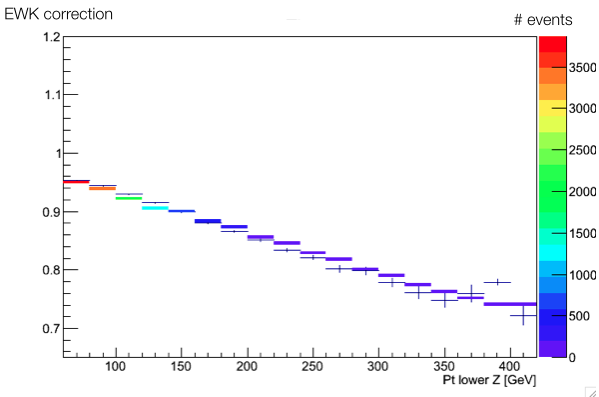
\includegraphics[width=0.60\textwidth]{figures/ZZ_ewkCorr.png}
\caption{Electroweak corrections applied as a function of $\hat{s}$, 
  $\hat{t}$, and of the quark flavours, provided by the authors of 
  Ref.~\cite{Bierweiler:2013dja}. The corrections thus computed are
  plotted as a function of the trailing boson \pt and compared to the
  average values of the corrections shown in Ref.~\cite{Bierweiler:2013dja} 
  for the ZZ process. The cross-shaped markers are obtained by
  applying the fully differential corrections, whereas the colored
  lines are taken from Ref.~\cite{Bierweiler:2013dja}.} 
\label{fig:ewkCorrectionCompare}
\end{figure}

\begin{figure}[htbp]
  \centering
  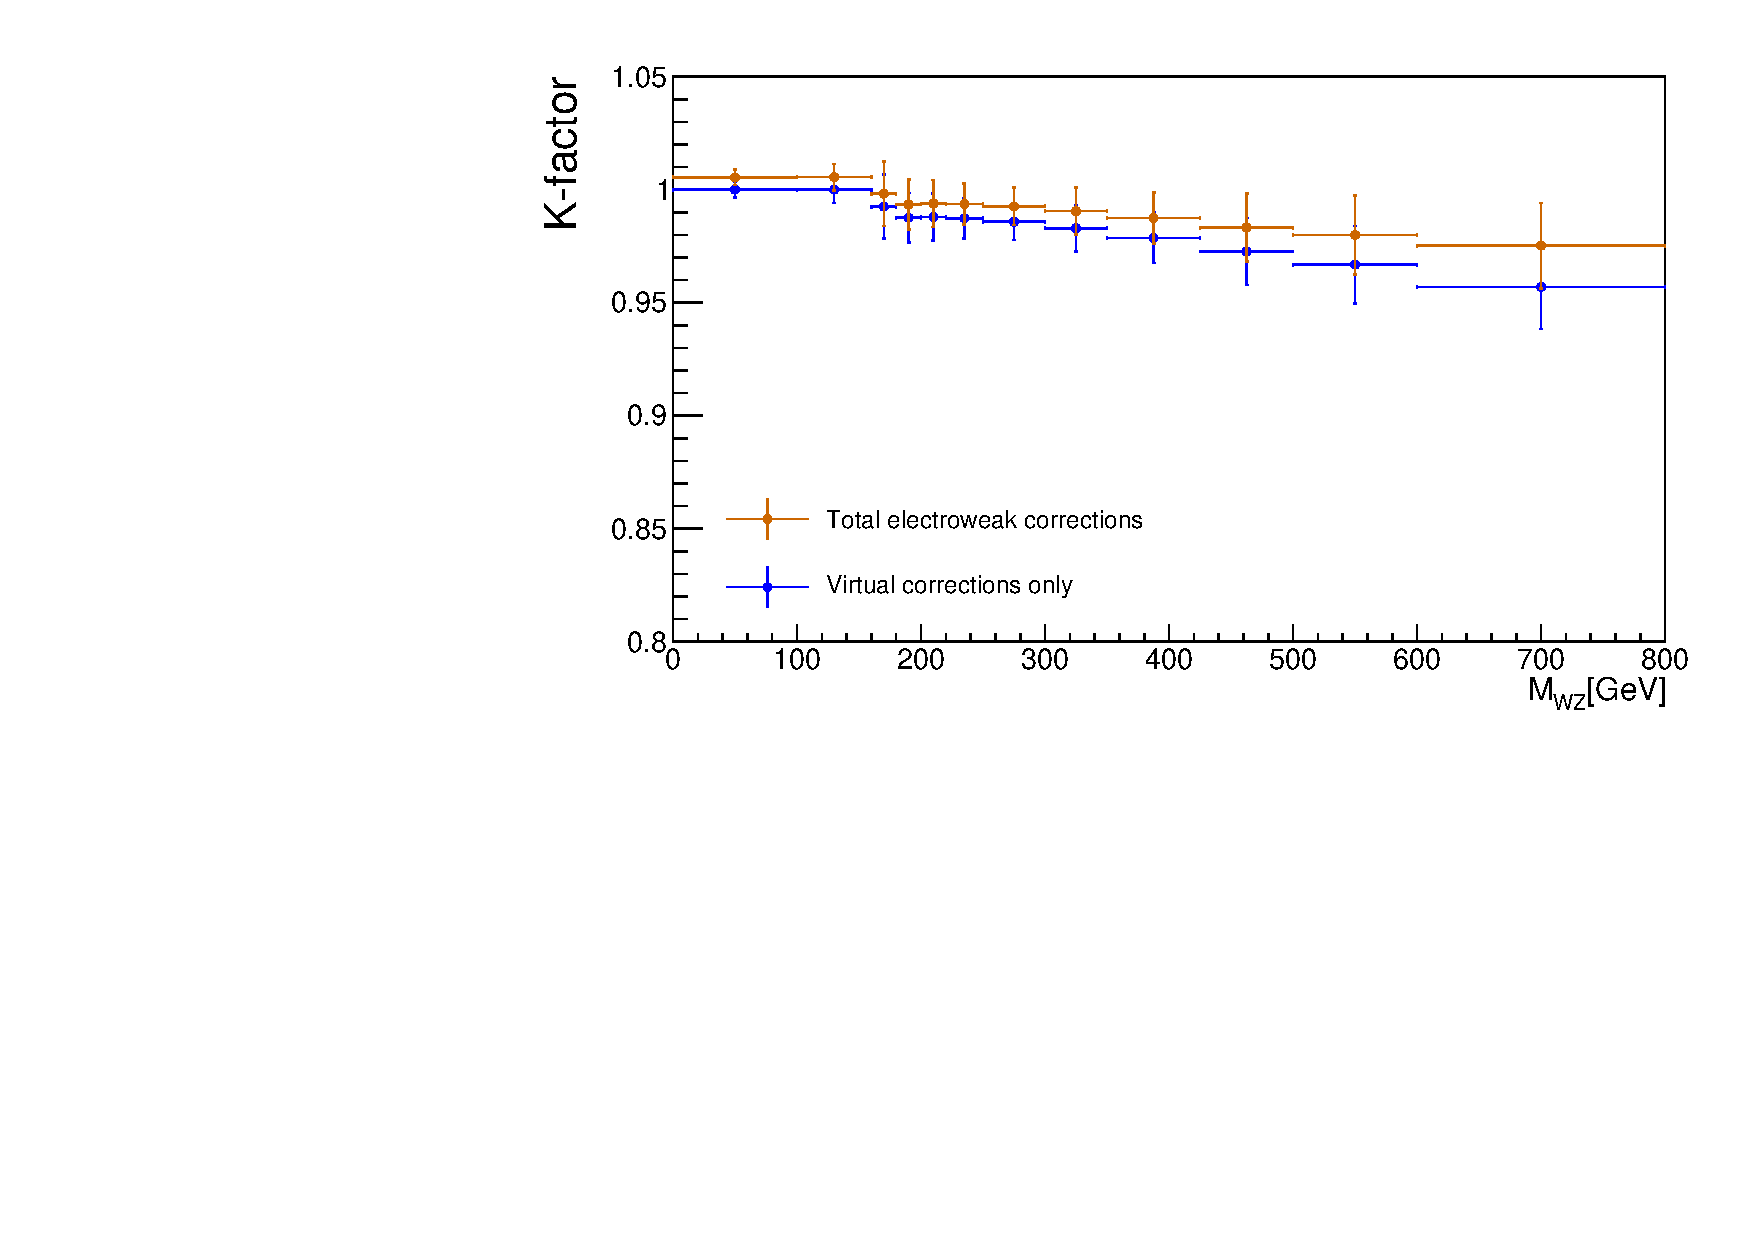
\includegraphics[width=0.49\textwidth]{figures/WZ_NLOEW_mWZ_ULB.pdf}
  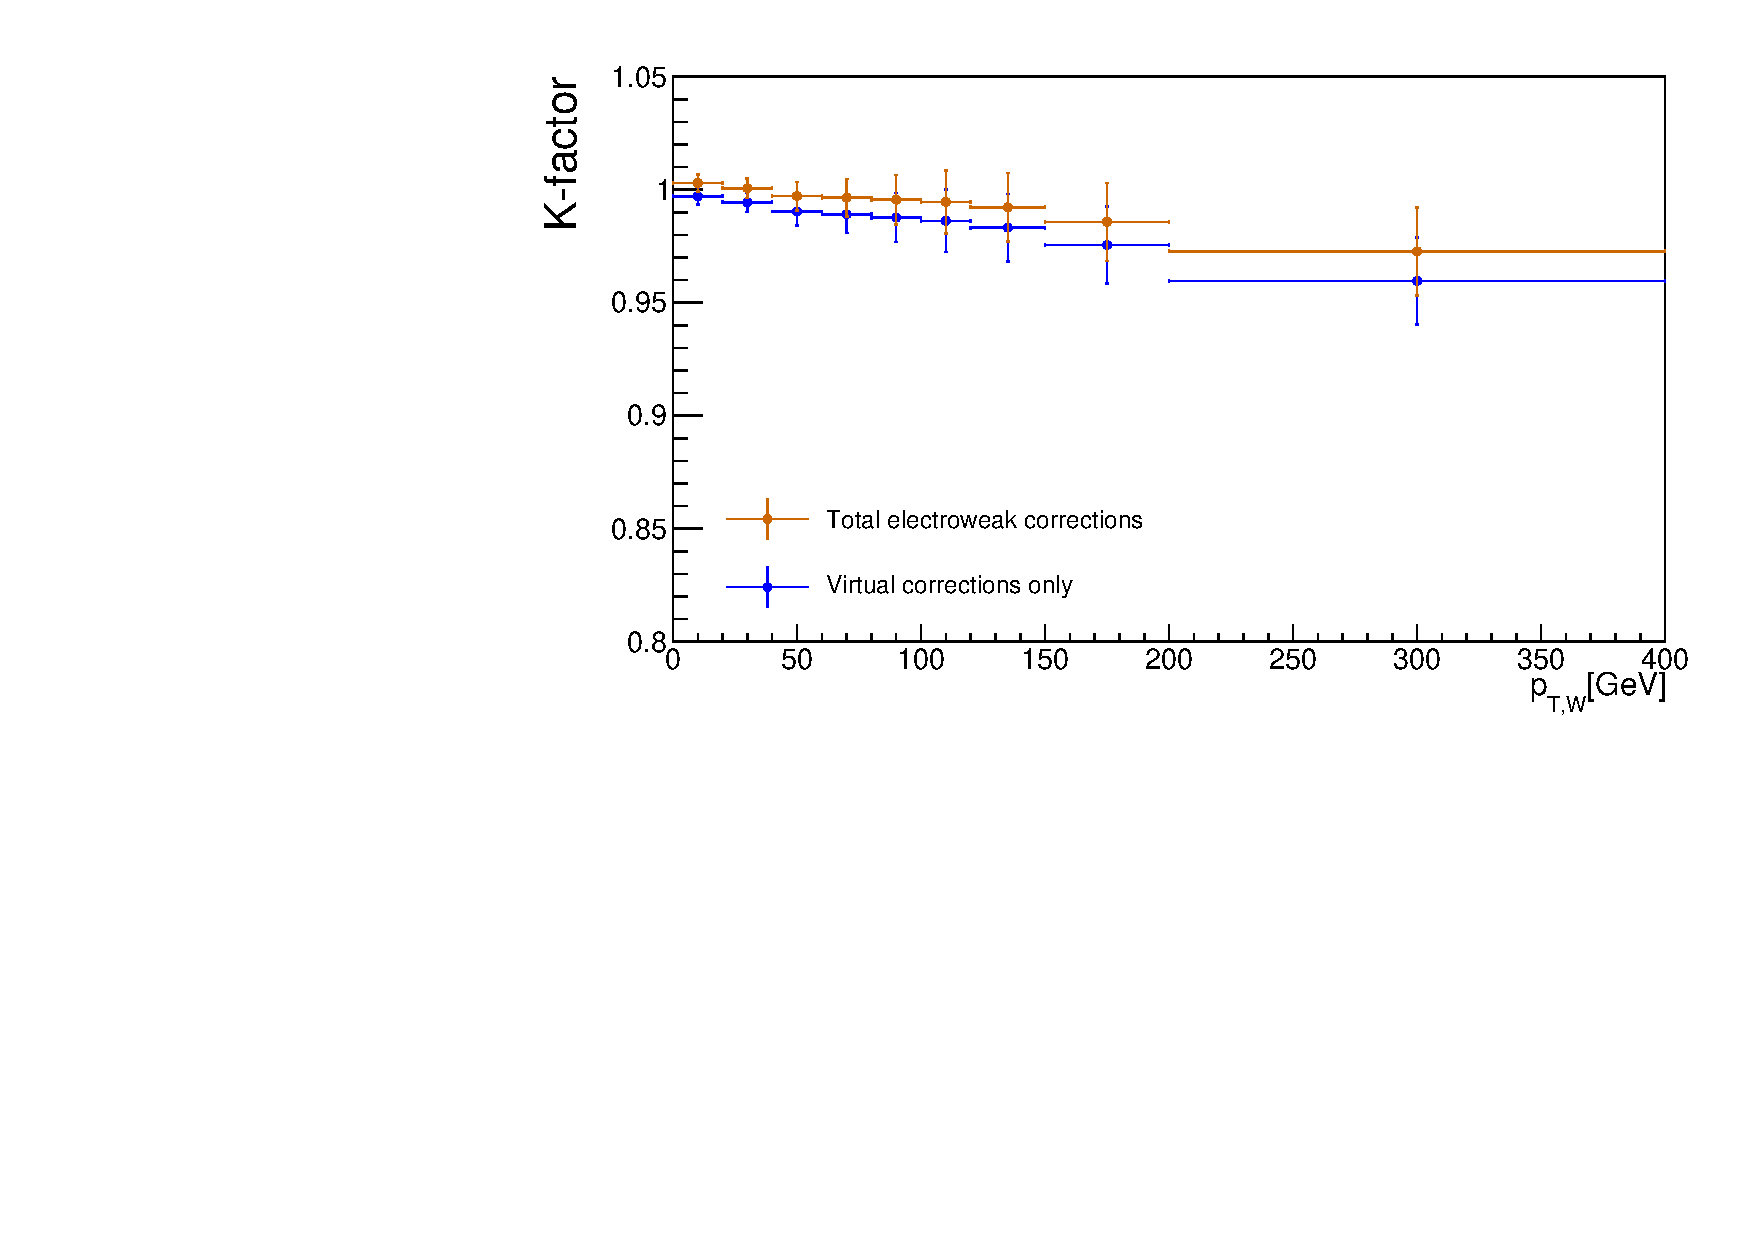
\includegraphics[width=0.49\textwidth]{figures/WZ_NLOEW_pTW_ULB.pdf}
  \caption{Evolution of the NLO electroweak corrections K-factor on $pp \to W^+Z$ as a function of $m_{WZ}$ (left) and $p_{T,W}$ (right), using only virtual corrections (blue) or using both virtual and photon-induced corrections (brown).
  \label{fig:gammaInduced_WZ}}
\end{figure}

\subsection{QCD corrections}
For quark-induced ZZ production, a QCD NLO to NNLO (next-to-next-to-leading order)
correction factor is applied as a function of the invariant mass of the two $\Z$ bosons,
$m_\mathrm{ZZ}$, at generator-level.
Figure~\ref{fig:NNLO_QCD_corrections} shows the differential cross section.
The correction is obtained using settings similar to the CMS simulation (dilepton mass requirements,
parton distribution function sets) to ensure its accuracy. See Ref.~\cite{Grazzini:2015hta}.
In the case of the $\W\Z$ process, a flat correction factor from QCD NLO to NNLO is applied.
Its value is $\mathbf{1.109}$; for details see Reference~\cite{Grazzini:2016swo}.

\begin{figure}[htp]
  \centering
  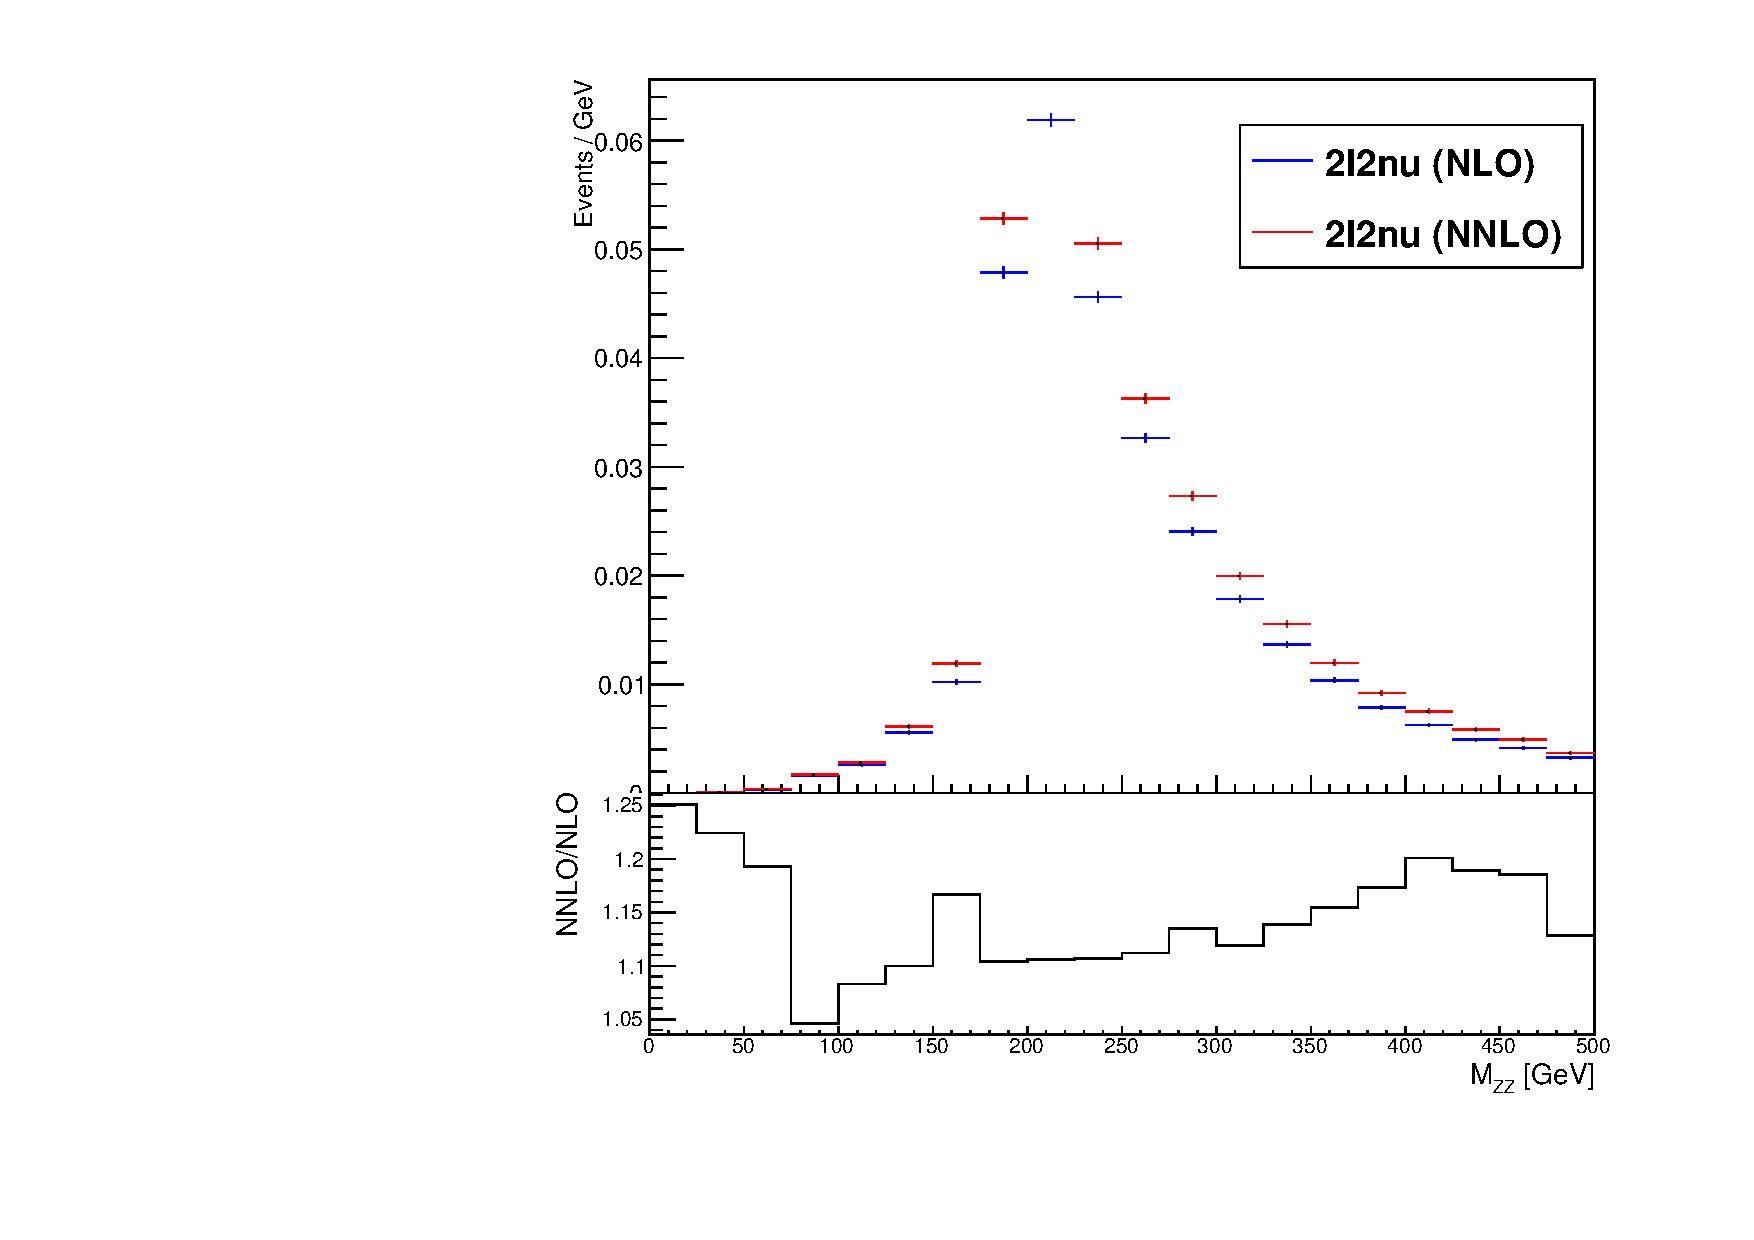
\includegraphics[width=0.49\textwidth]{figures/ZZ_NNLO_QCD_corrections.pdf} 
  \caption{Evolution of the NNLO QCD corrections K-factor for $pp \to ZZ \to 2\ell2\nu$ as a function of $m_\mathrm{ZZ}$ at generator-level.} 
  \label{fig:NNLO_QCD_corrections}
\end{figure} 

\subsection{Cross terms}

As discussed in Refs.~\cite{Bierweiler:2013dja,Gieseke:2014gka}, terms purely of higher
order in $\alpha_{\mathrm{EW}}$ are expected to be negligible.
A significant uncertainty, instead, stems from missing
QCD-EW combined corrections, \eg involving two-loop terms of order
$\alpha_{\mathrm{S}}\alpha_{\mathrm{EW}}$.
So far, this contribution from diagrams at NLO in both QCD and electroweak has been ignored.
This is the source of the so-called ``QCD-electroweak cross-term.''

The electroweak and QCD corrections are both large in magnitude, for the ZZ process, 
so the QCD-electroweak cross-term cannot be neglected.
It is only understood to the level of $25\%$.

For the majority of ZZ events which have little hadronic activity, the
uncertainty from such missing QCD-EW combined corrections is
estimated from the product of the NLO QCD corrections 
($1+\delta_{\mathrm{QCD}}$) and NLO EW corrections
($1+\delta_{\mathrm{EW}}$), as
$\delta_{\mathrm{QCD}}\delta_{\mathrm{EW}}$. To compute this 
uncertainty, a flat $\delta_{\mathrm{QCD}}$ value of
$0.6$ is considered , while $\delta_{\mathrm{EW}}$ is computed event-by-event as a
function of the lower-\Z \pt (cf. Sec.~\ref{sec:higher-order-corrections}), then we
vary the event weight by a factor
$(1+\delta_{\mathrm{QCD}}\delta_{\mathrm{EW}})$.

Since the EW $k$-factors for the ZZ are strictly valid only when the hadronic
activity in the event is moderate, a variable $\rho$ is built to estimate the level of
hadronic activity in the event, following Ref.~\cite{Gieseke:2014gka}.
$\rho$ is calculated by considering the balance of the generated leptons' transverse momenta: 
\begin{equation}
\label{eq:the_rho}
\rho = \frac{\left|\vec{\pt}(\ell_1)+\vec{\pt}(\ell_2)+\vec{\pt}(\ell_3)+\vec{\pt}(\ell_4)\right|}{\left|\vec{\pt}(\ell_1)\right|+\left|\vec{\pt}(\ell_2)\right|+\left|\vec{\pt}(\ell_3)\right|+\left|\vec{\pt}(\ell_4)\right|}
\end{equation} 
For events with $\rho>0.3$, \ie with a significant imbalance in the
transverse momenta of the four leptons due to the presence of jets,
an increased uncertainty of 100\% on the EW correction for that given
event is assigned---in other words, the factor 
$(1+\delta_{\mathrm{QCD}}\delta_{\mathrm{EW}})$ is replaced with 
$(1+\delta_{\mathrm{EW}})$ when computing the variations of the weights.
At high boson momentum, less than 1\% of the ZZ events have $\rho>0.3$.

The overall electroweak NLO correction to the $\W\Z$ process is relatively small~\cite{Bierweiler:2013dja,Gieseke:2014gka,Baglio:113005}.
This is because the virtual corrections and photon-induced corrections partially cancel.
Therefore, the NLO QCD-electroweak cross-term for the $\W\Z$ process is also small.
The uncertainties on the NLO electroweak calculation can be estimated as the size of the NLO QCD-electroweak cross terms~\cite{Manohar:2016nzj,Alwall:2014hca,Frixione:2014qaa,Frixione:2015zaa}.

\begin{figure}[hb] % WZ NLO EW
 \centering
 \begin{tikzpicture} % WZ at NLO EW (s-channel) internal loop
  \begin{feynman}
   \vertex (q1) {\(\boldsymbol{\Pq}\)};
   \vertex [below= 3cm of q1] (q2) {\(\boldsymbol{\Paq'}\)};
   \vertex [right= 1.5cm of q1] (a1);
   \vertex [below= 1.5cm of a1] (a2);
   \vertex [right= 1.6cm of a2] (b1);
   \vertex [right= 1.6cm of b1] (c1);
   \vertex [above= 1.3cm of c1] (c2);
   \vertex [below= 1.3cm of c1] (c3);
   \vertex [right= 1cm of c2] (d1);
   \vertex [right= 1cm of c3] (d2);
   \vertex [above= 0.3cm of d1] (f1) {\(\boldsymbol{\ell}\)};
   \vertex [below= 0.3cm of d1] (f2) {\(\boldsymbol{\bar{\ell}}\)};
   \vertex [above= 0.3cm of d2] (f3) {\(\boldsymbol{\ell}\)};
   \vertex [below= 0.3cm of d2] (f4) {\(\boldsymbol{\bar{\nu_\ell}}\)};
   \vertex [below right= 0.9cm of q1] (V1);
   \vertex [above right= 0.9cm of q2] (V2);
   
   \diagram* {
    (q1) -- [fermion, very thick] (a2),
    (q2) -- [anti fermion, very thick] (a2),
    (a2) -- [boson, very thick, edge label'=\(\boldsymbol{\PWm}\)] (b1),
    (b1) -- [boson, very thick, edge label=\(\boldsymbol{\Z}\)] (c2),
    (b1) -- [boson, very thick, edge label=\(\boldsymbol{\PWm}\)] (c3),
    (c2) -- [fermion, very thick] (f1),
    (c2) -- [anti fermion, very thick] (f2),
    (c3) -- [fermion, very thick] (f3),
    (c3) -- [anti fermion, very thick] (f4),
    (V1) -- [boson, very thick, edge label'=\(\boldsymbol{\Z/\W/\gamma}\)] (V2),
   };
  \end{feynman}
 \end{tikzpicture} \hspace{1cm}
 \begin{tikzpicture} % WZ at NLO (t-channel) internal loop
  \begin{feynman}
   \vertex (q1) {\(\boldsymbol{\Pq}\)};
   \vertex [below= 2cm of q1] (q2) {\(\boldsymbol{\Paq'}\)};
   \vertex [right= 2cm of q1] (a);
   \vertex [right= 2cm of q2] (b);
   \vertex [right= 2cm of a] (c);
   \vertex [right= 2cm of b] (d);
   \vertex [right= 1.5cm of c] (e);
   \vertex [right= 1.5cm of d] (f);
   \vertex [above= 0.3cm of e] (f1) {\(\boldsymbol{\ell}\)};
   \vertex [below= 0.3cm of e] (f2) {\(\boldsymbol{\bar{\ell}}\)};
   \vertex [above= 0.3cm of f] (f3) {\(\boldsymbol{\nu_\ell}\)};
   \vertex [below= 0.3cm of f] (f4) {\(\boldsymbol{\bar{\ell}}\)};
   \vertex [right= 0.8cm of q2] (V1);
   \vertex [above= 0.7cm of b] (V2);
   
   \diagram* {
    (q1) -- [fermion, very thick] (a),
    (q2) -- [anti fermion, very thick] (b),
    (a) -- [fermion, very thick] (b),
    (a) -- [boson, very thick, edge label'=\(\boldsymbol{\Z}\)] (c),
    (b) -- [boson, very thick, edge label'=\(\boldsymbol{\W^+}\)] (d),
    (c) -- [fermion, very thick] (f1),
    (c) -- [anti fermion, very thick] (f2),
    (d) -- [fermion, very thick] (f3),
    (d) -- [anti fermion, very thick] (f4),
    (V1) -- [boson, very thick, bend left, edge label=\(\boldsymbol{\Z/\W/\gamma}\)] (V2),
   };
  \end{feynman}
 \end{tikzpicture} \vspace{1cm}

 \begin{tikzpicture} % WZ at NLO EW (s-channel) y-induced
  \begin{feynman}
   \vertex (y1) {\(\boldsymbol{\gamma}\)};
   \vertex [below= 3cm of y1] (q2) {\(\boldsymbol{\Pq}\)};
   \vertex [right= 1.5cm of q1] (a1);
   \vertex [below= 1.5cm of a1] (a2);
   \vertex [right= 1.6cm of a2] (b1);
   \vertex [right= 1.6cm of b1] (c1);
   \vertex [above= 1.3cm of c1] (c2);
   \vertex [below= 1.3cm of c1] (c3);
   \vertex [right= 1cm of c2] (d1);
   \vertex [right= 1cm of c3] (d2);
   \vertex [above= 0.3cm of d1] (f1) {\(\boldsymbol{\ell}\)};
   \vertex [below= 0.3cm of d1] (f2) {\(\boldsymbol{\bar{\ell}}\)};
   \vertex [above= 0.3cm of d2] (f3) {\(\boldsymbol{\ell}\)};
   \vertex [below= 0.3cm of d2] (f4) {\(\boldsymbol{\bar{\nu_\ell}}\)};
   \vertex [below right= 1.2cm of y1] (y2);
   \vertex [right= 1cm of y2] (fsrq1);
   \vertex [above= 0.6cm of fsrq1] (fsrq2) {\(\boldsymbol{\Pq'}\)};
   
   \diagram* {
    (y1) -- [boson, very thick] (y2),
    (y2) -- [anti fermion, very thick] (a2),
    (q2) -- [fermion, very thick] (a2),
    (a2) -- [boson, very thick, edge label'=\(\boldsymbol{\PWm}\)] (b1),
    (b1) -- [boson, very thick, edge label=\(\boldsymbol{\Z}\)] (c2),
    (b1) -- [boson, very thick, edge label=\(\boldsymbol{\PWm}\)] (c3),
    (c2) -- [fermion, very thick] (f1),
    (c2) -- [anti fermion, very thick] (f2),
    (c3) -- [fermion, very thick] (f3),
    (c3) -- [anti fermion, very thick] (f4),
    (y2) -- [fermion, very thick] (fsrq2),
   };
  \end{feynman}
 \end{tikzpicture} \hspace{1cm}
 \begin{tikzpicture} % WZ at NLO EW (t-channel) y-induced
  \begin{feynman}
   \vertex (y1) {\(\boldsymbol{\gamma}\)};
   \vertex [right= 1cm of y1] (y2);
   \vertex [below= 0.3cm of y2] (y3);
   \vertex [right= 1.8cm of y3] (fsrq1);
   \vertex [above= 0.2cm of fsrq1] (fsrq2) {\(\boldsymbol{\Pq'}\)};
   \vertex [below= 3.6cm of y1] (q2) {\(\boldsymbol{\Pq}\)};
   \vertex [right= 1cm of y3] (a1);
   \vertex [below= 0.5cm of a1] (a2);
   \vertex [right= 2cm of q2] (a3);
   \vertex [above= 0.8cm of a3] (a4);
   \vertex [right= 2cm of a2] (c);
   \vertex [right= 2cm of a4] (d);
   \vertex [right= 1.5cm of c] (e);
   \vertex [right= 1.5cm of d] (f);
   \vertex [above= 0.3cm of e] (f1) {\(\boldsymbol{\ell}\)};
   \vertex [below= 0.3cm of e] (f2) {\(\boldsymbol{\bar{\ell}}\)};
   \vertex [above= 0.3cm of f] (f3) {\(\boldsymbol{\nu_\ell}\)};
   \vertex [below= 0.3cm of f] (f4) {\(\boldsymbol{\bar{\ell}}\)};
   
   \diagram* {
    (y1) -- [boson, very thick] (y3),
    (y3) -- [anti fermion, very thick] (a2),
    (q2) -- [fermion, very thick] (a4),
    (a2) -- [anti fermion, very thick] (a4),
    (a2) -- [boson, very thick, edge label'=\(\boldsymbol{\Z}\)] (c),
    (a4) -- [boson, very thick, edge label'=\(\boldsymbol{\PWp}\)] (d),
    (c) -- [fermion, very thick] (f1),
    (c) -- [anti fermion, very thick] (f2),
    (d) -- [fermion, very thick] (f3),
    (d) -- [anti fermion, very thick] (f4),
    (y3) -- [fermion, very thick] (fsrq2),
   };
  \end{feynman}
 \end{tikzpicture}  
 

 \caption{WZ production at NLO in EW by internal loop processes (upper row) and photon-quark induced processes (lower row).} \label{fig:WZNLO}
\end{figure}

Yet another conservative step is taken regarding the NNLO QCD corrections.
For lack of a better method, the PDF and QCD scale uncertainties from the original POWHEG calculation at NLO in QCD are carried forward,
even though the final distributions are corrected to NNLO in QCD.
This represents another setback in the understanding of the diboson processes.

\clearpage
\section{Visible ZZ process}
\label{sec:zz4l}
Here, I will describe how events are selected to observe the fully visible ZZ process.
Two Z boson candidates are each formed from a pair of opposite-charge electrons or muons having invariant mass within 15 \GeV of the Z boson mass resonance (91.1876 \GeV).
The Z candidate whose invariant mass is closer to the Z mass is denoted as $\mathrm{Z}_1$; the other, as $\mathrm{Z}_2$.
In total, there are four well-identified leptons, giving a very high purity selection.
Therefore neither hadronic $\tau$ nor b-jet vetoes are applied.
The minimum dilepton invariant mass, considering all pairs, must be greater than 4 \GeV.
The purpose of this is to reject the so-called ``nonprompt'' backgrounds, which I will explain next.

There is triboson contamination which is the resonant contribution from three bosons (WWZ, WZZ, ZZZ), or two top quarks and a Z boson.
There is also a small amount of contamination from the nonprompt backgrounds,
including but not limited to the Drell-Yan process, semileptonic diboson decays, leptonic WW decays, and ditop production.
From these, it is still possible to end up with four charged leptons or fake lepton signatures after the hard process.
These have been mostly suppressed by the minimum dilepton mass requirement.
Last but not least, there are Standard Model Higgs boson decays to four leptons
via $\mathrm{H}\rightarrow \mathrm{ZZ^*} \rightarrow 4\ell$, 
but the cross section is comparatively small.

The selection yields in simulation and data for this ZZ analysis are shown in Table~\ref{tab:zz4lyields}.
Distributions of illustrative variables after the selection are shown in Figures~\ref{fig:zz4l_mll},~\ref{fig:zz4l_zpt}, and~\ref{fig:zz4l_moreplots}.

\begin{figure}[!hb]
\centering
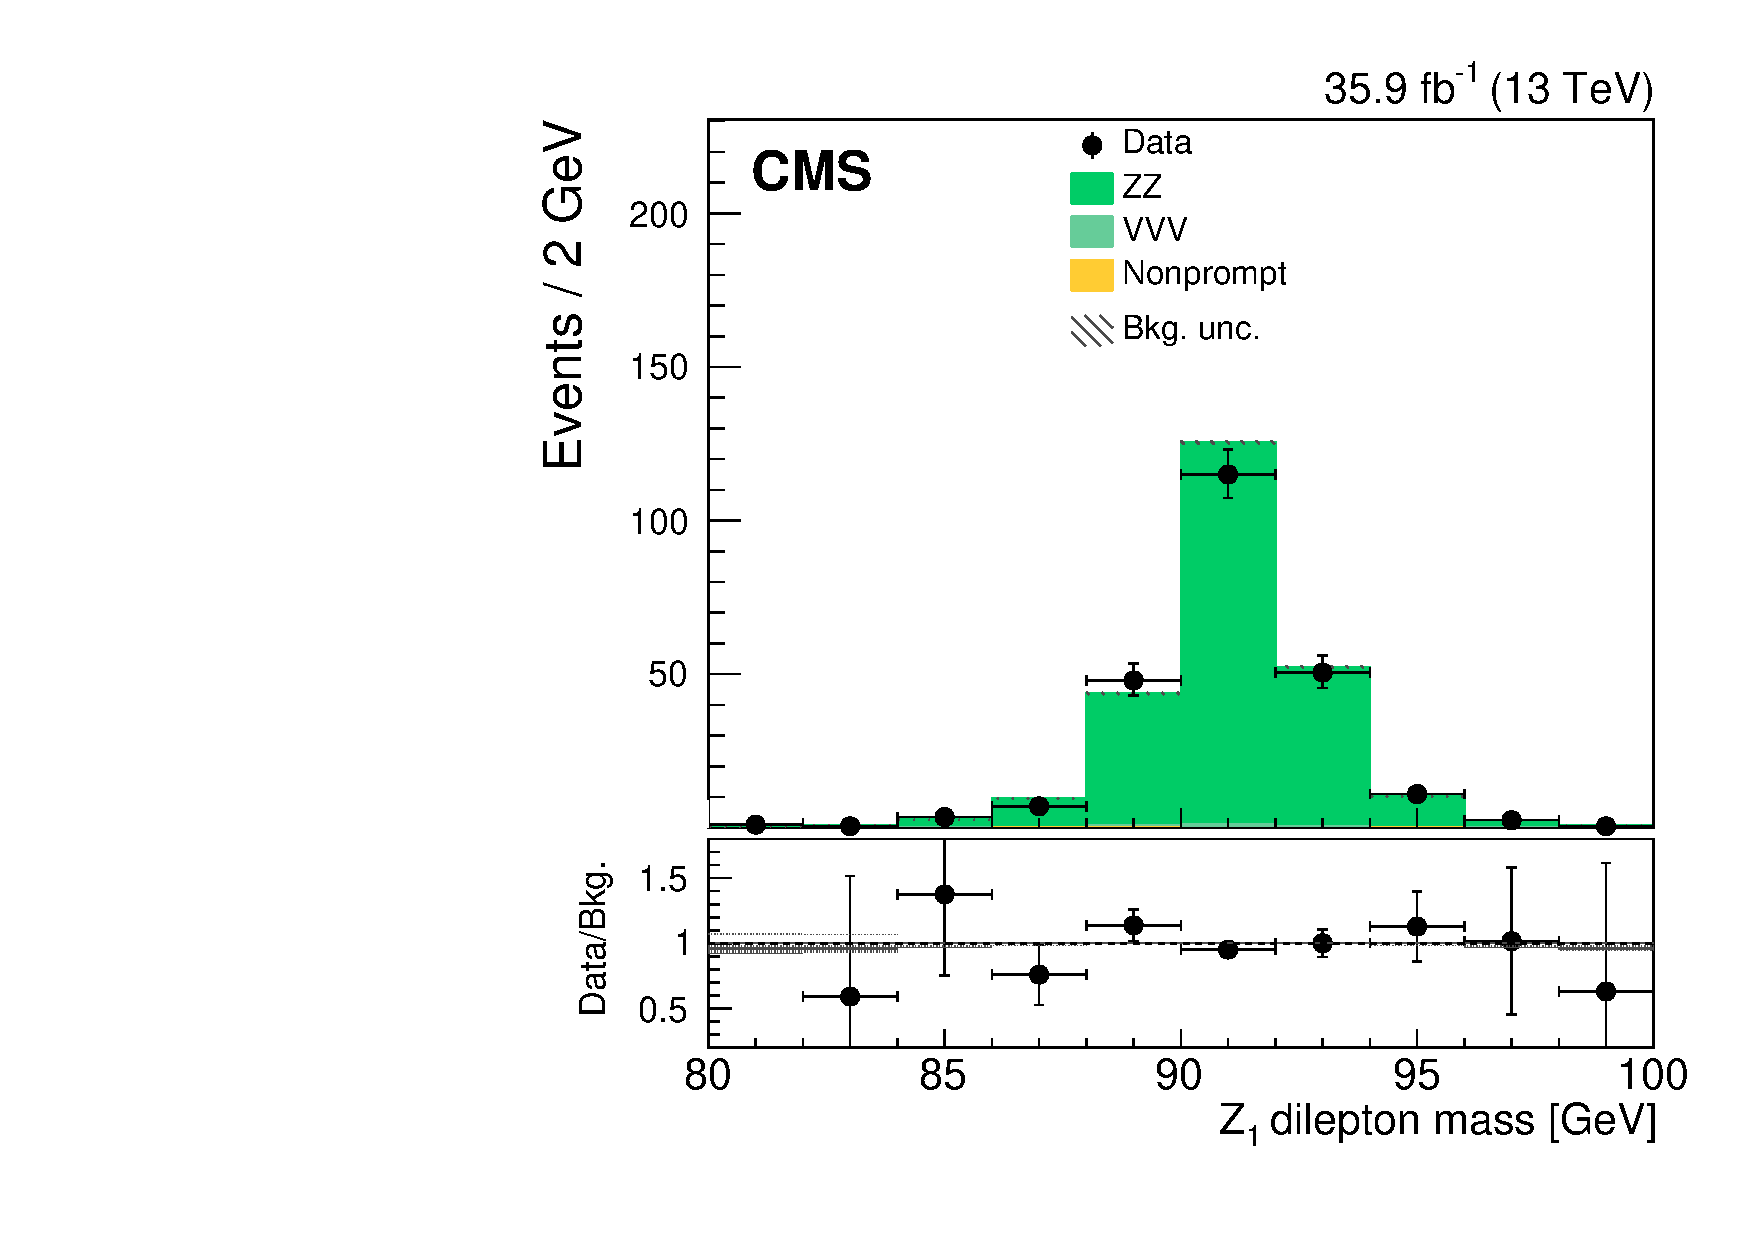
\includegraphics[width=0.48\textwidth]{figures/dibosons/zz4l/mZ1.pdf}
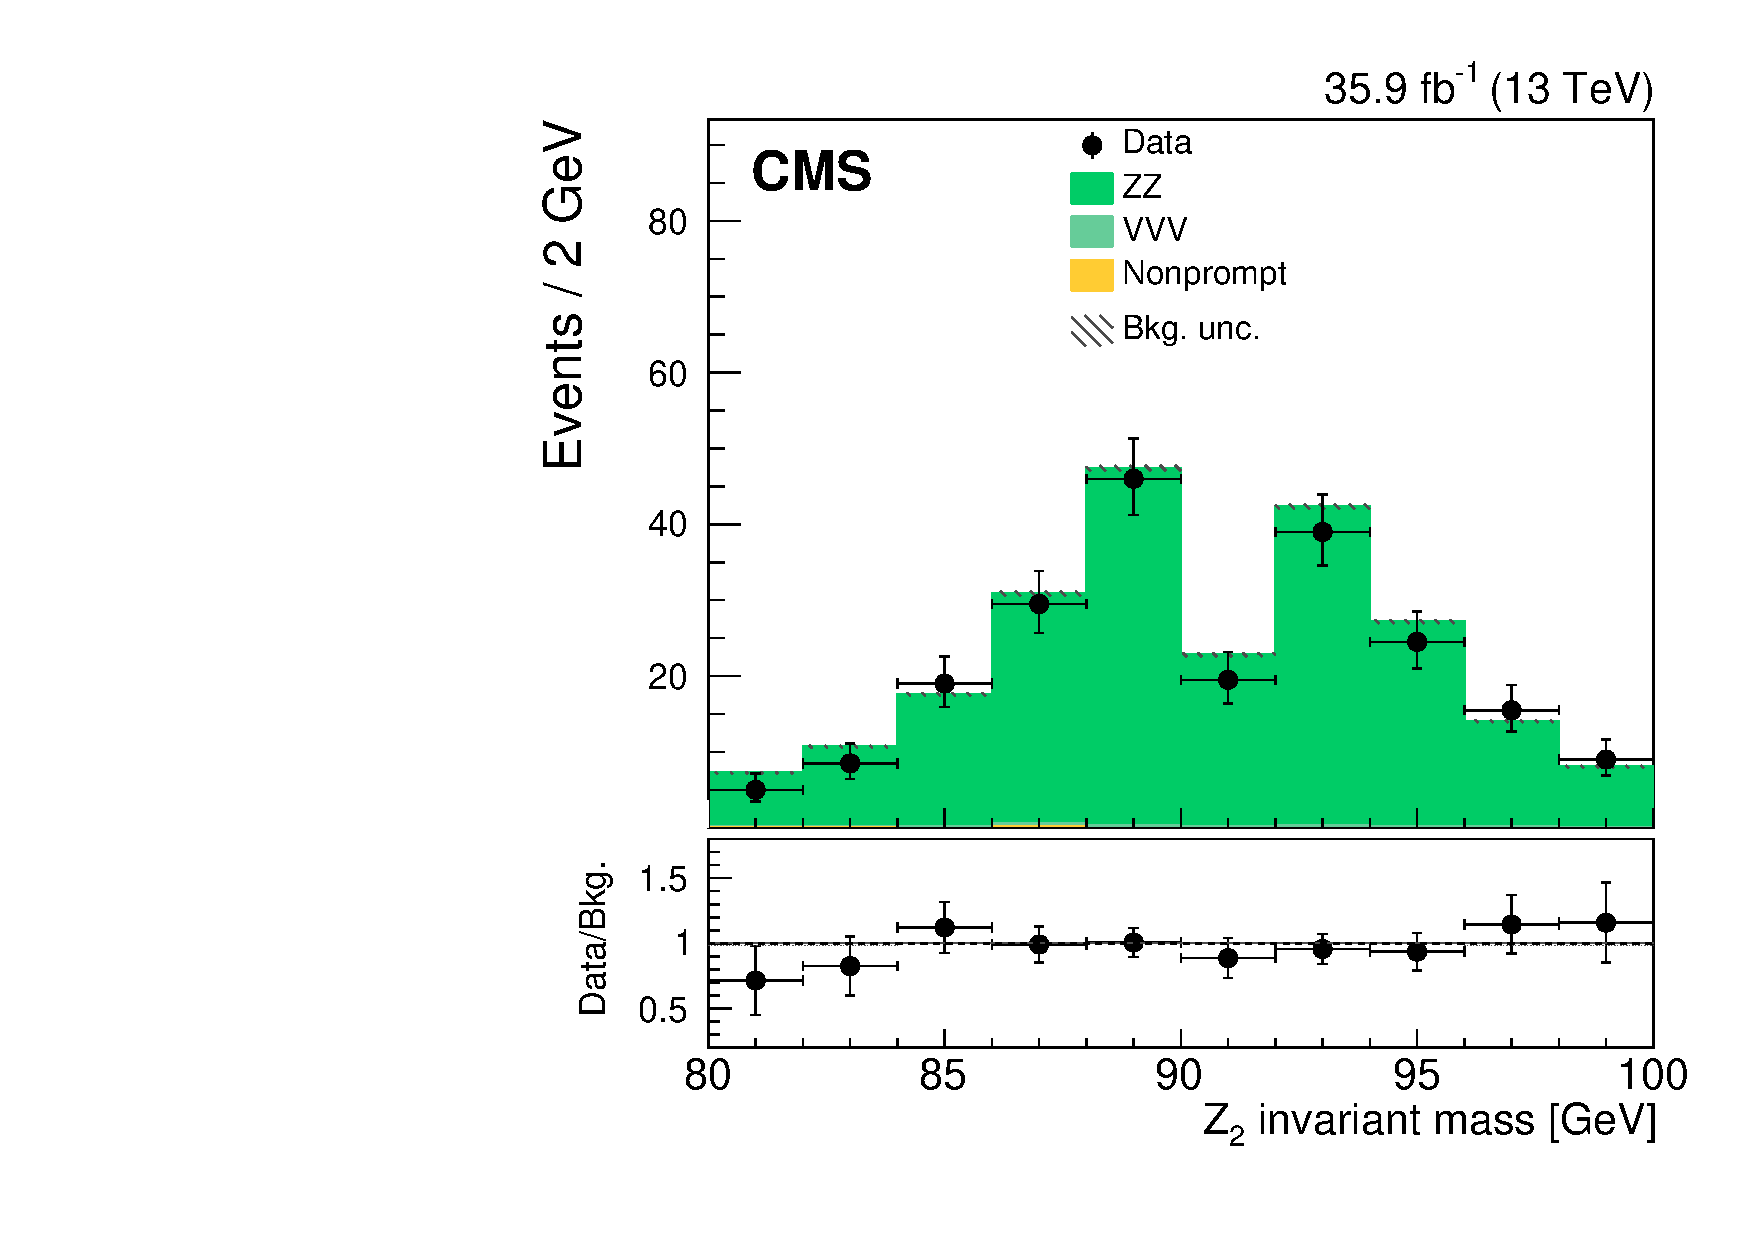
\includegraphics[width=0.48\textwidth]{figures/dibosons/zz4l/mZ2.pdf}
\caption{The invariant masses of the two Z candidates. 
In the right plot, the distribution of $\mathrm{Z}_{2}$ has a cavity close to the Z mass pole because of how $\mathrm{Z}_{1,2}$ are defined.
\label{fig:zz4l_mll}}
\end{figure}

%(..Data):    81.00 +/-   9.00 |   175.00 +/-  13.23 |   224.00 +/-  14.97 |     0.00 +/-   0.00 ->   480.00 +/-  21.91
%(....EM):     0.13 +/-   0.10 |     0.11 +/-   0.10 |     0.66 +/-   0.40 |     0.00 +/-   0.00 ->     0.90 +/-   0.42
%(Zgamma):     0.00 +/-   0.00 |     0.00 +/-   0.00 |     0.00 +/-   0.00 |     0.00 +/-   0.00 ->     0.00 +/-   0.00
%(....WZ):     0.00 +/-   0.00 |     0.00 +/-   0.00 |     0.00 +/-   0.00 |     0.00 +/-   0.00 ->     0.00 +/-   0.00
%( ...ZZ):    77.56 +/-   0.63 |   171.40 +/-   0.96 |   243.01 +/-   1.12 |     0.00 +/-   0.00 ->   491.96 +/-   1.61
%(...VVV):     1.02 +/-   0.12 |     1.94 +/-   0.16 |     2.54 +/-   0.20 |     0.00 +/-   0.00 ->     5.50 +/-   0.28
%(.Higgs):     0.06 +/-   0.18 |     0.41 +/-   0.20 |     0.32 +/-   0.18 |     0.00 +/-   0.00 ->     0.79 +/-   0.32
%(...bkg):    78.77 +/-   0.67 |   173.85 +/-   1.00 |   246.52 +/-   1.22 |     0.00 +/-   0.00 ->   499.15 +/-   1.71
\setlength{\tabcolsep}{12pt}
\begin{table}[!t]
  \caption{Predicted and observed number of events for the ZZ four-lepton selection using $\usedLumi$.
  Only statistical uncertainties are reported.
  \label{tab:zz4lyields}}
  \begin{center}
{\scriptsize
  \begin{tabular}{rllll}
\hline 
Process & $4e$ & $4\mu$ & $2e2\mu$ & Total \\
\hline
ZZ                    &   77.6 $\pm$  0.6 &  171.4 $\pm$  1.0 &  243.0 $\pm$     1.1 &  492.0 $\pm$     1.6 \\ 
VVV                   &    1.0 $\pm$  0.1 &    1.9 $\pm$  0.2 &    2.5 $\pm$     0.2 &    5.5 $\pm$     0.3 \\ 
Nonprompt bkg.        &    0.1 $\pm$  0.1 &    0.1 $\pm$  0.1 &    0.7 $\pm$     0.4 &    0.9 $\pm$     0.4 \\ 
Higgs                 &    0.1 $\pm$  0.1 &    0.4 $\pm$  0.2 &    0.3 $\pm$     0.2 &    0.8 $\pm$     0.3 \\ 
\hline                                                                               
Total                 &   78.7 $\pm$  0.7 &  173.4 $\pm$  1.0 &  246.5 $\pm$     1.2 &  499.2 $\pm$     1.7 \\
\hline                                                                               
Data                  &   81              &  175              &  224                 &  480                 \\
\hline
  \end{tabular}
}
  \end{center}
\end{table}


\begin{figure}[!b]
\centering
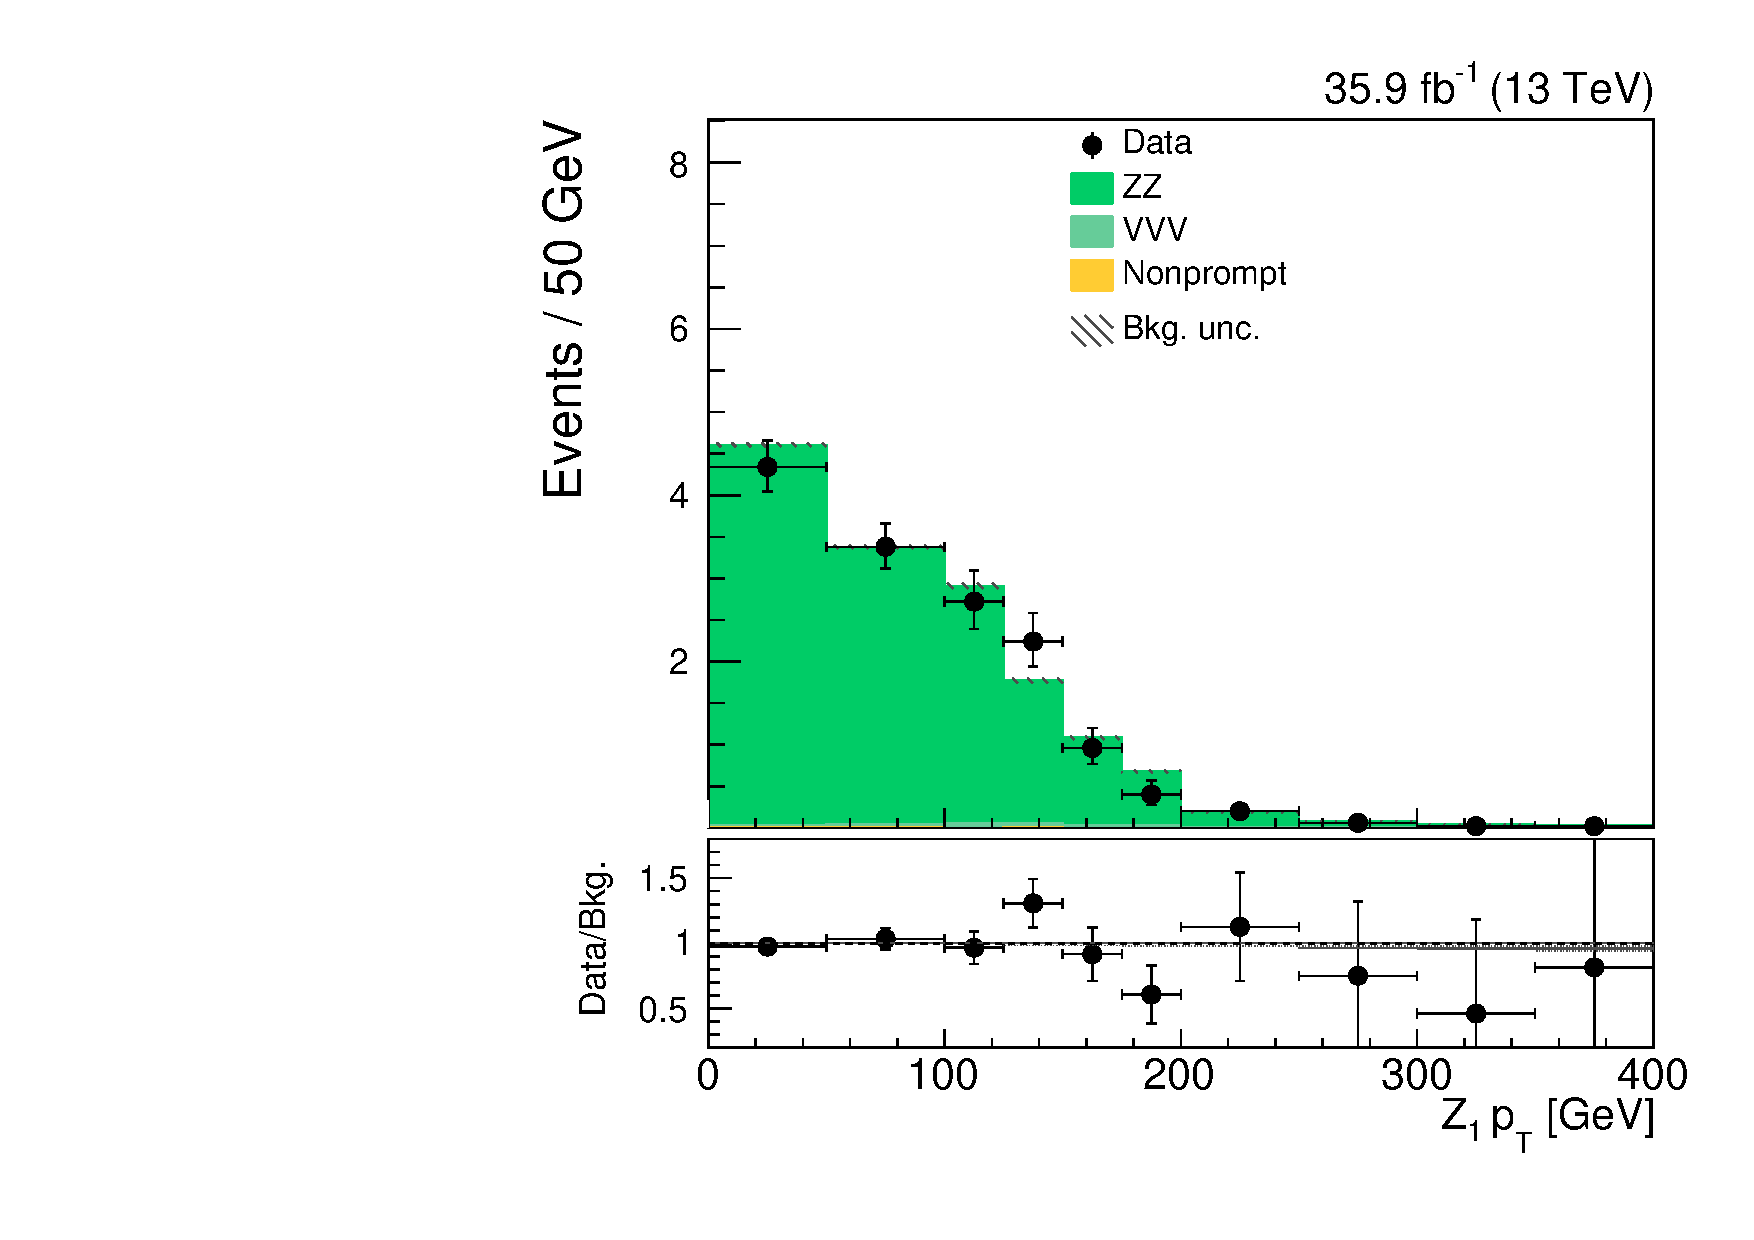
\includegraphics[width=0.48\textwidth]{figures/dibosons/zz4l/pTZ1.pdf}
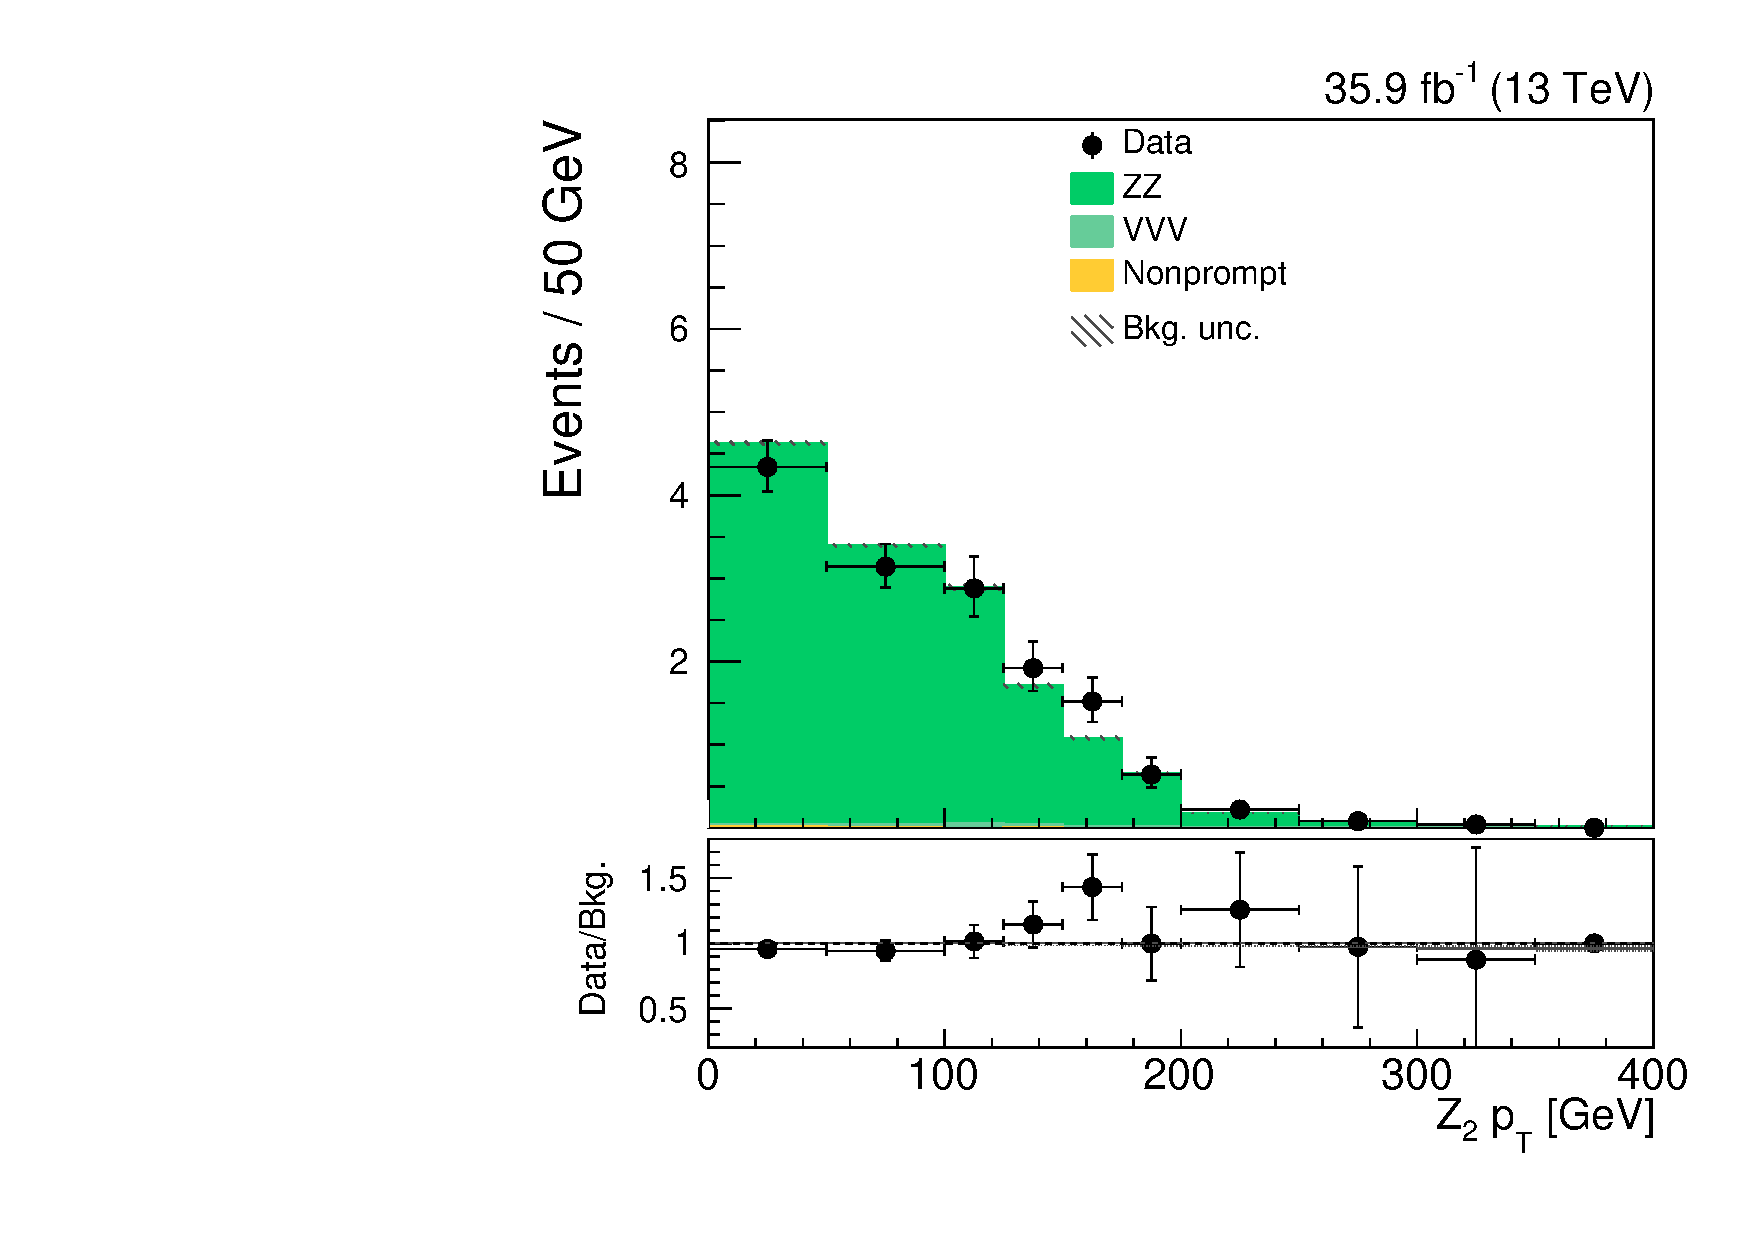
\includegraphics[width=0.48\textwidth]{figures/dibosons/zz4l/pTZ2.pdf}
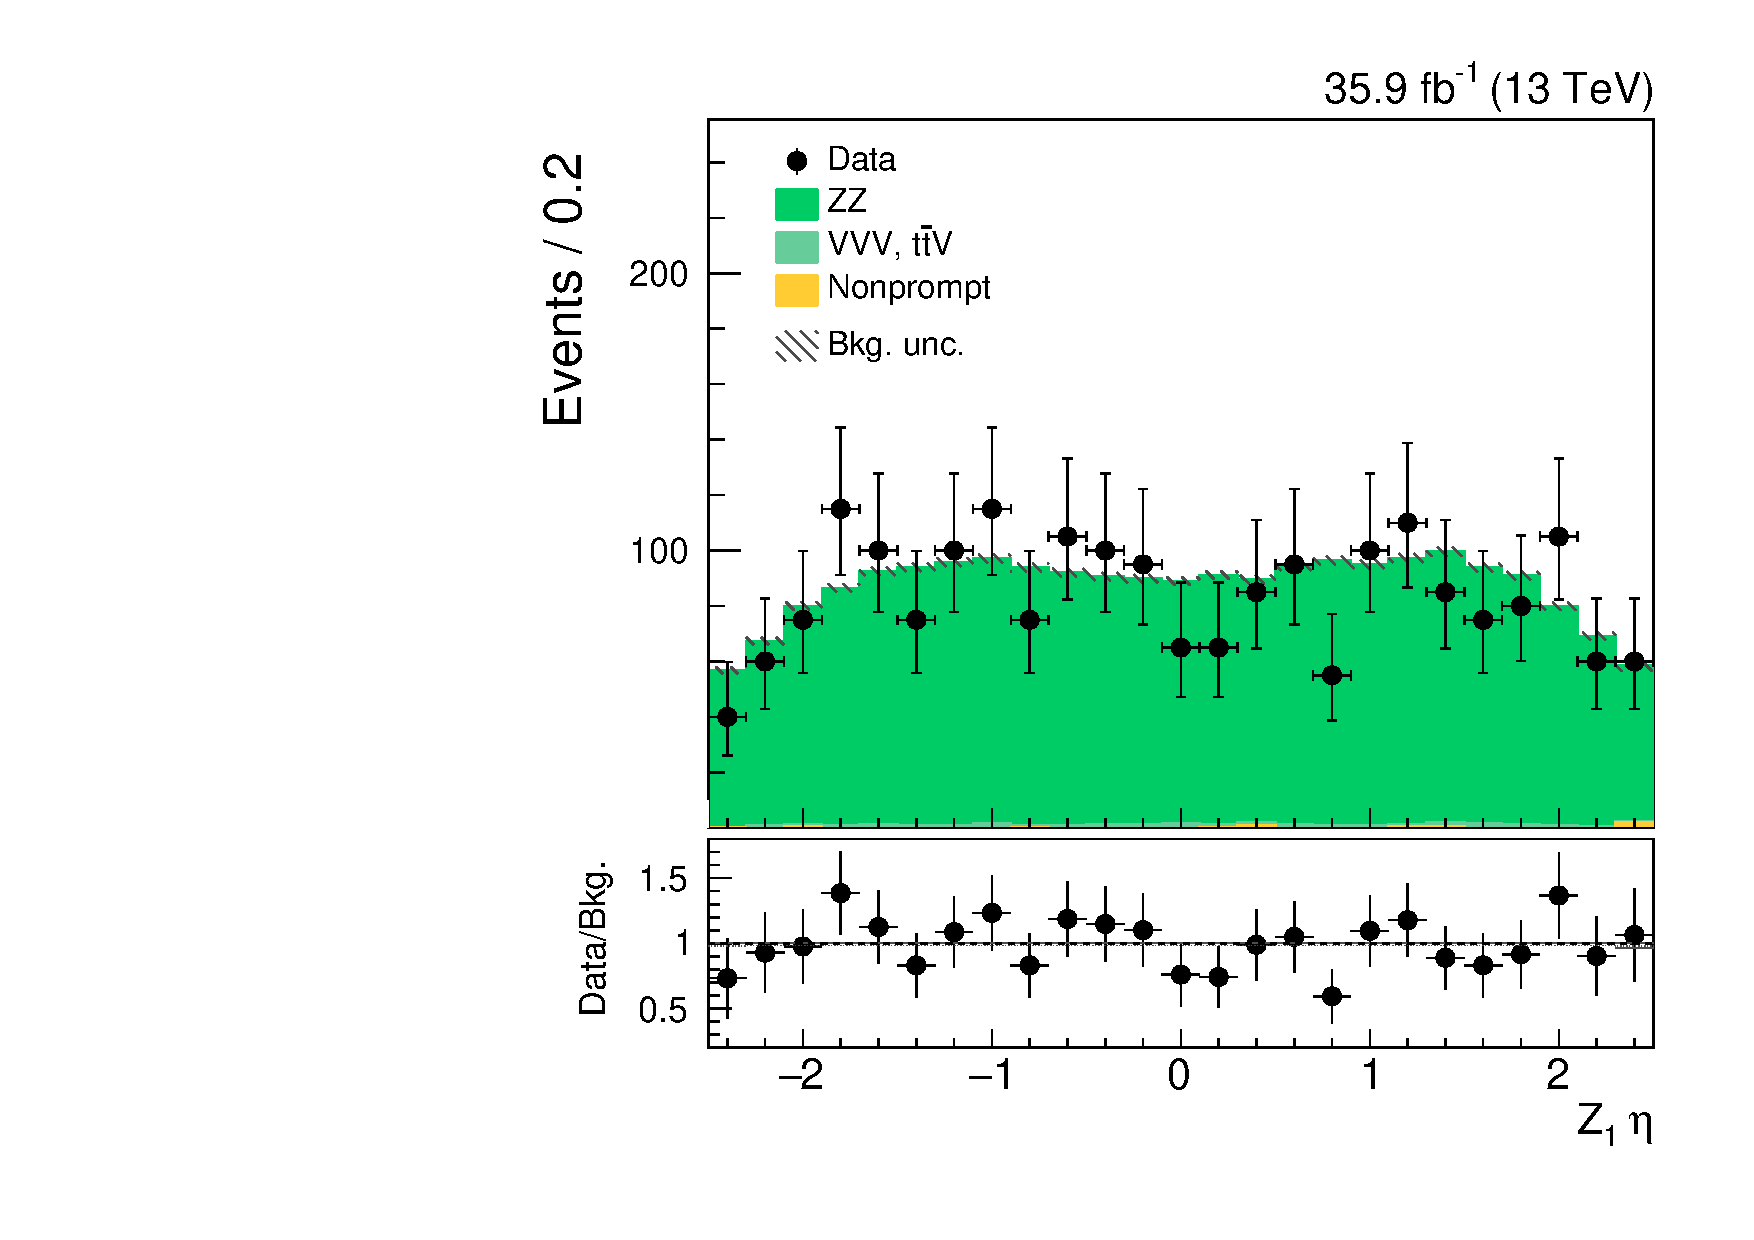
\includegraphics[width=0.48\textwidth]{figures/dibosons/zz4l/etaZ1.pdf}
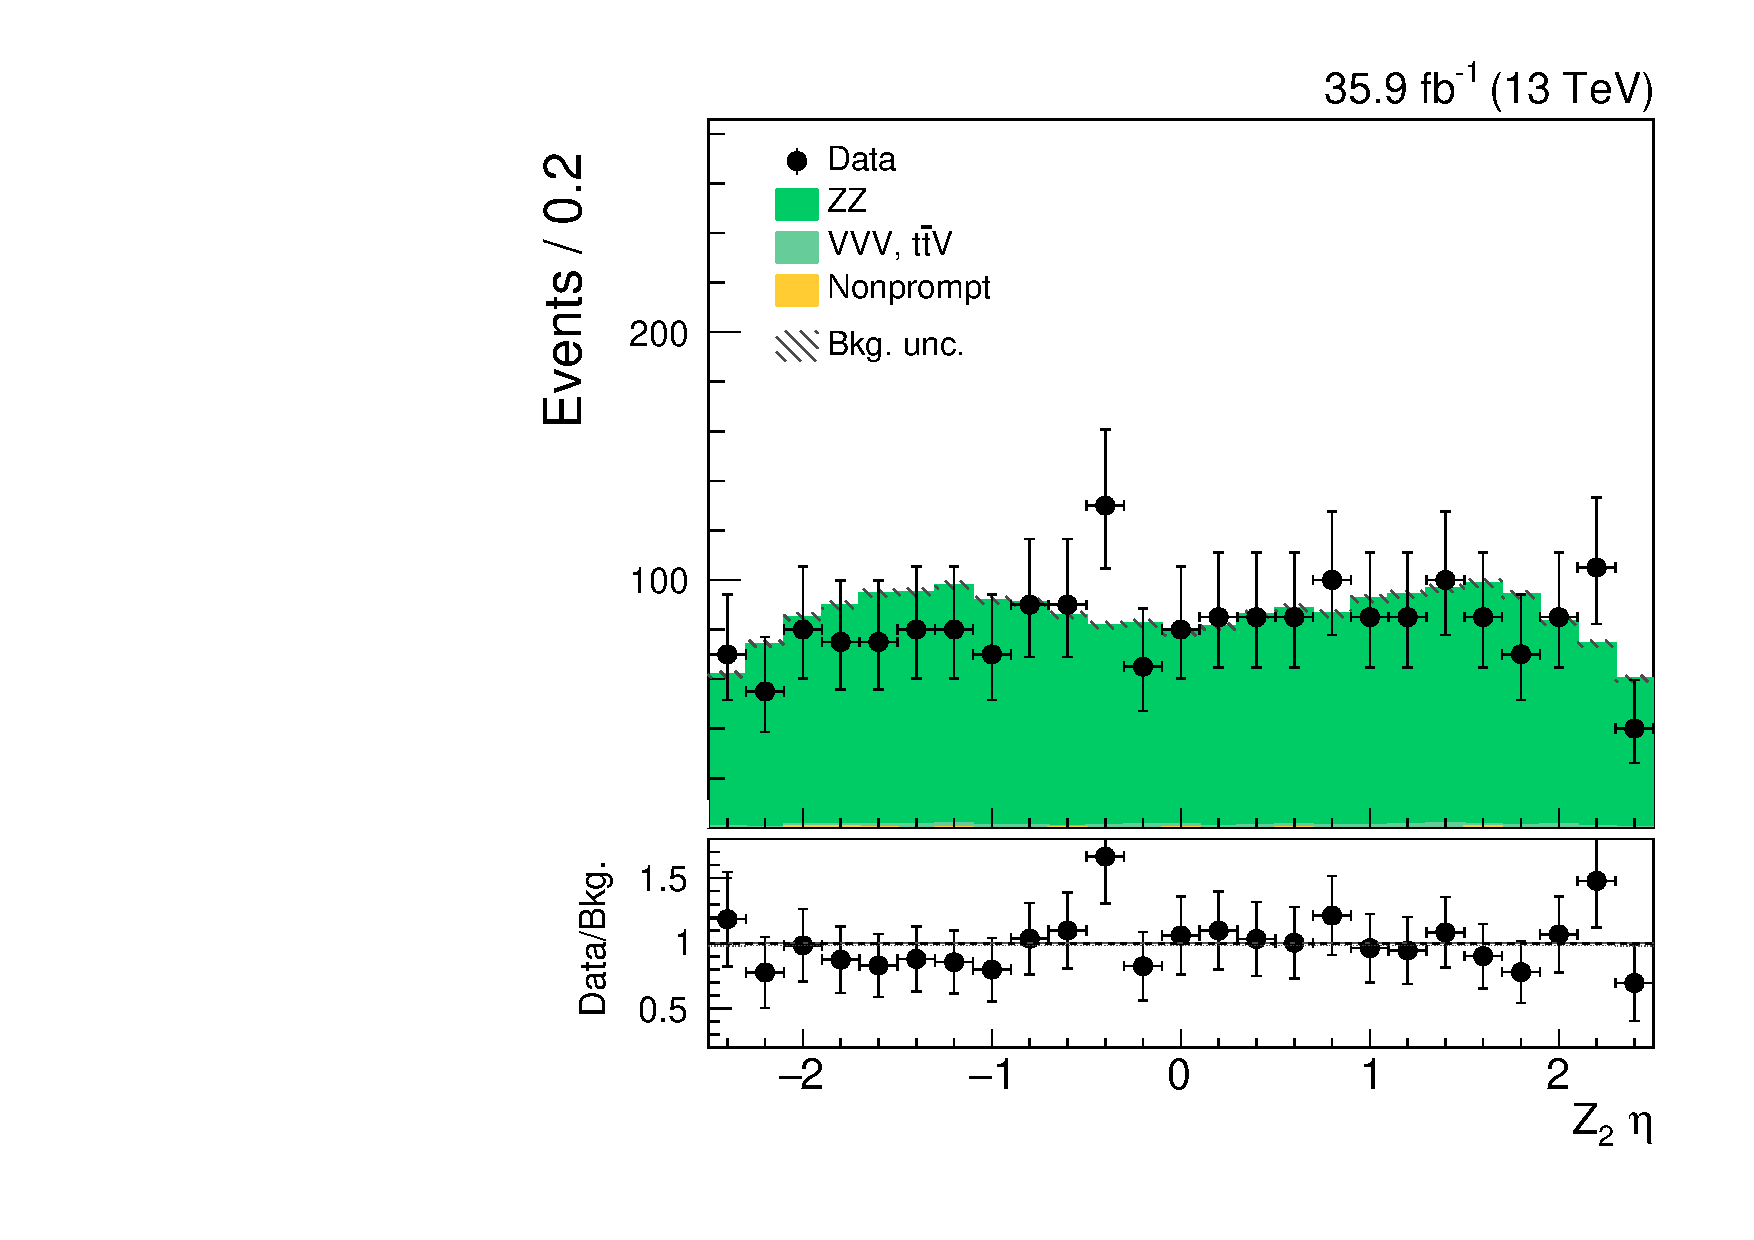
\includegraphics[width=0.48\textwidth]{figures/dibosons/zz4l/etaZ2.pdf}
\caption{Kinematics of the Z candidates. Top: their transverse momenta. Bottom: their pseudorapidities.
\label{fig:zz4l_zpt}}
\end{figure}

\clearpage
\begin{figure}[!h]
\centering
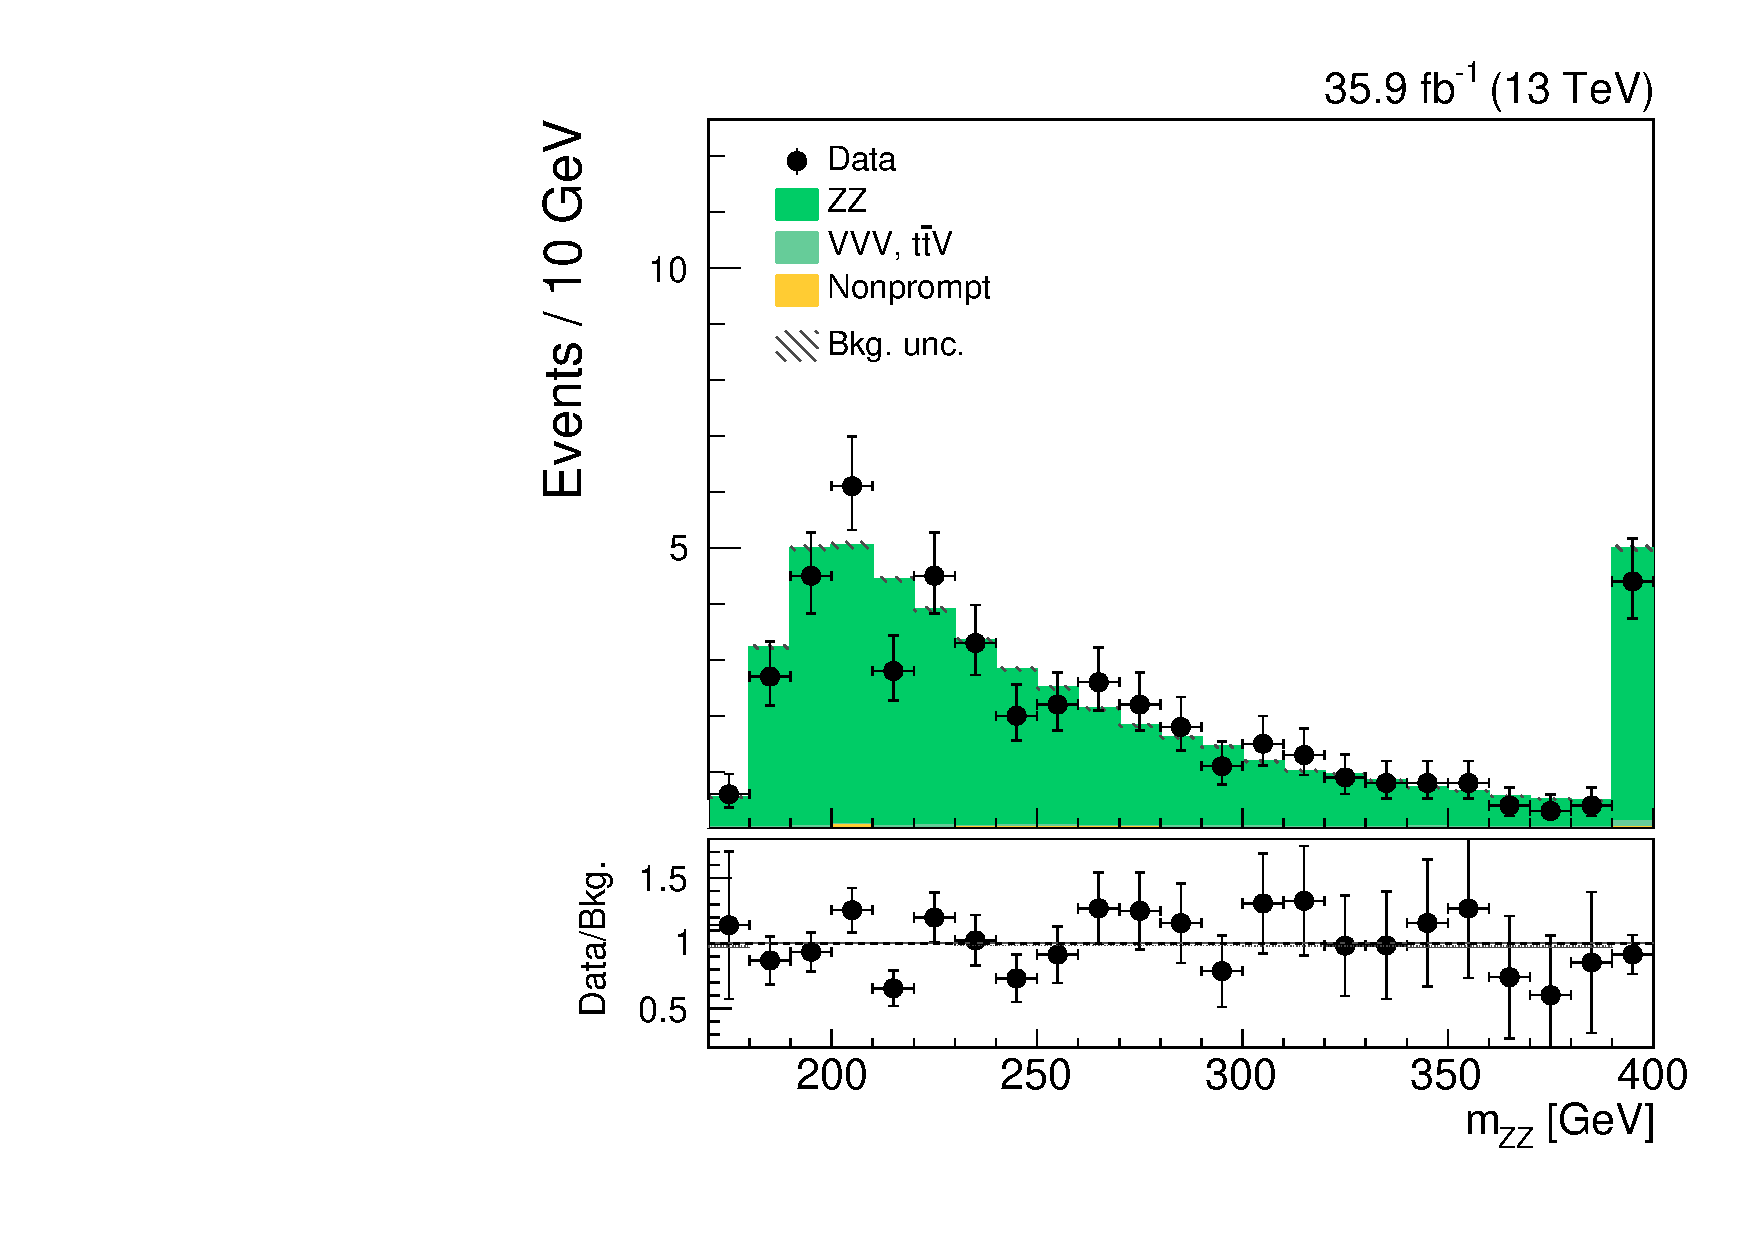
\includegraphics[width=0.48\textwidth]{figures/dibosons/zz4l/mZZ.pdf}
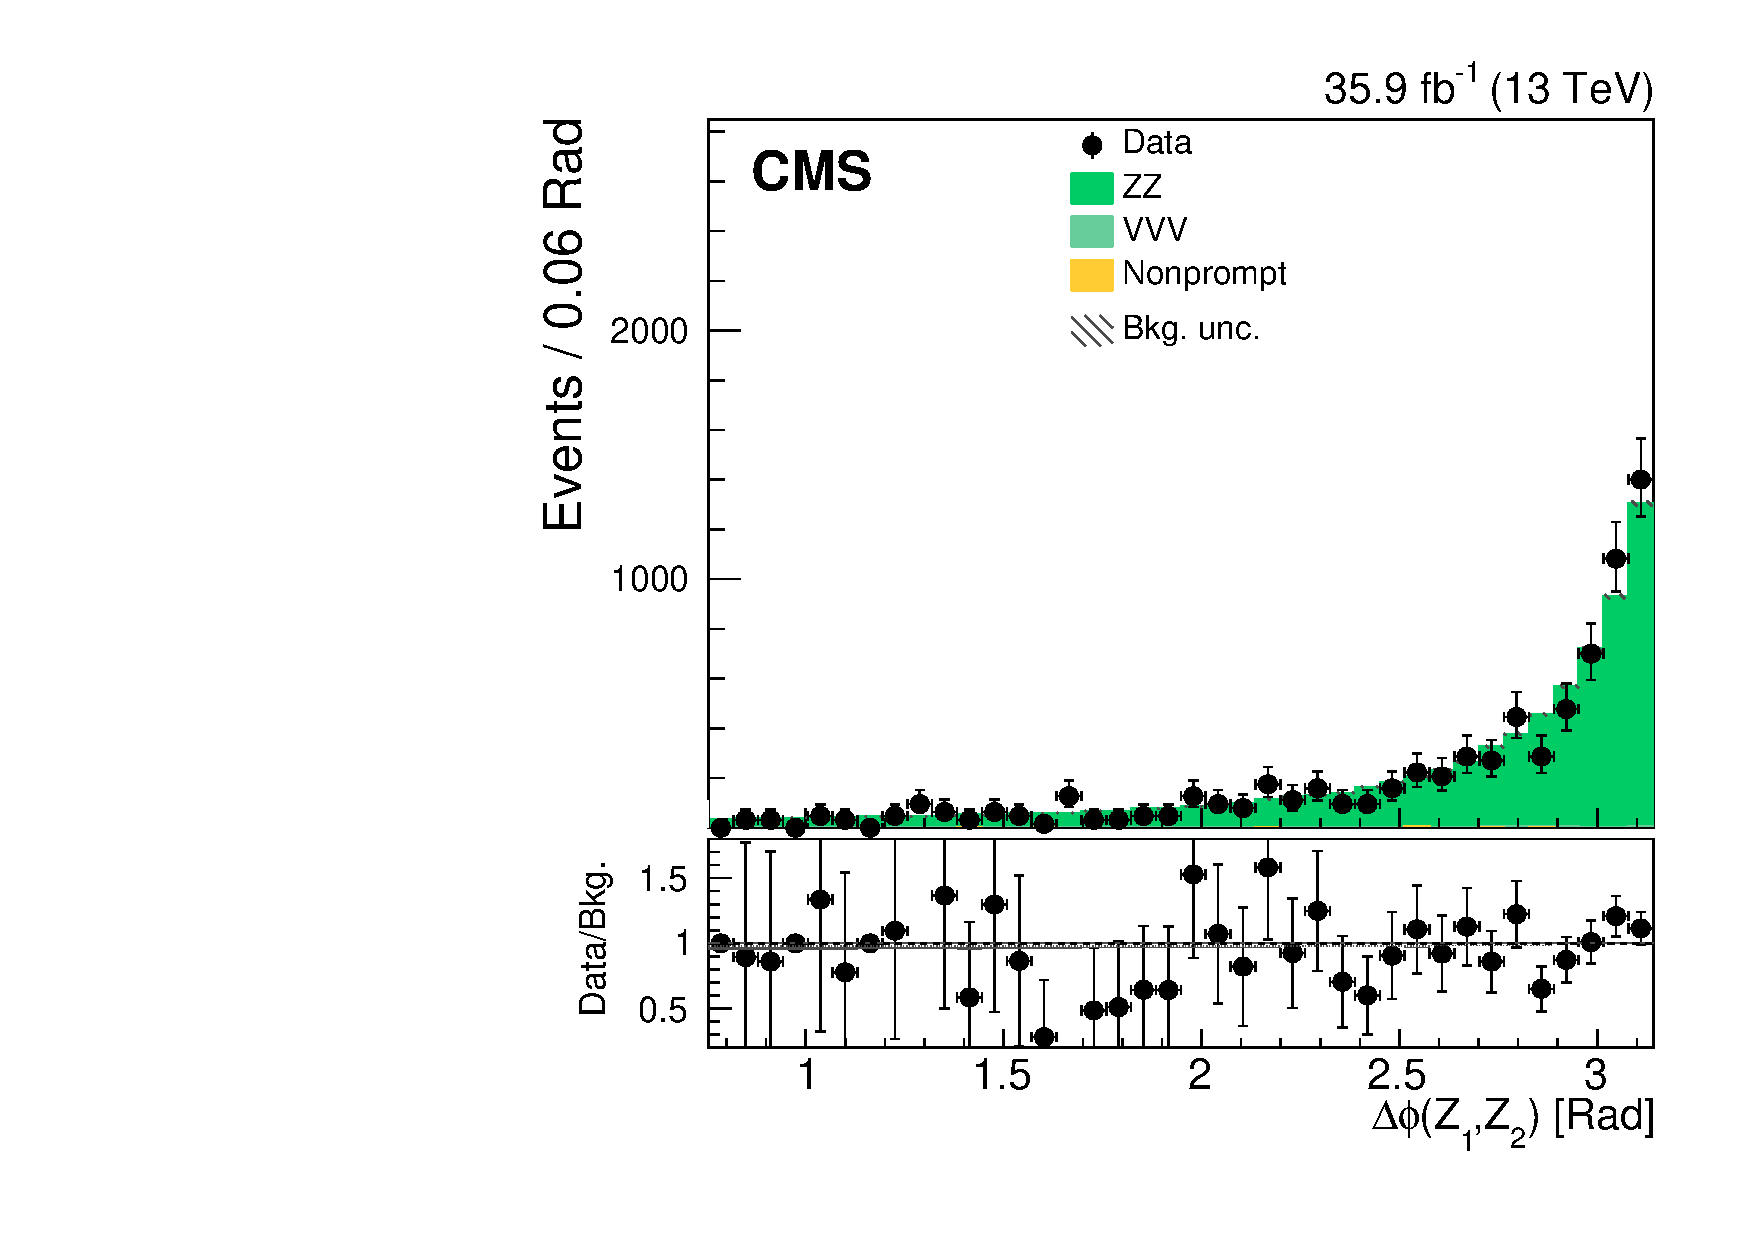
\includegraphics[width=0.48\textwidth]{figures/dibosons/zz4l/dphiZZ.pdf}
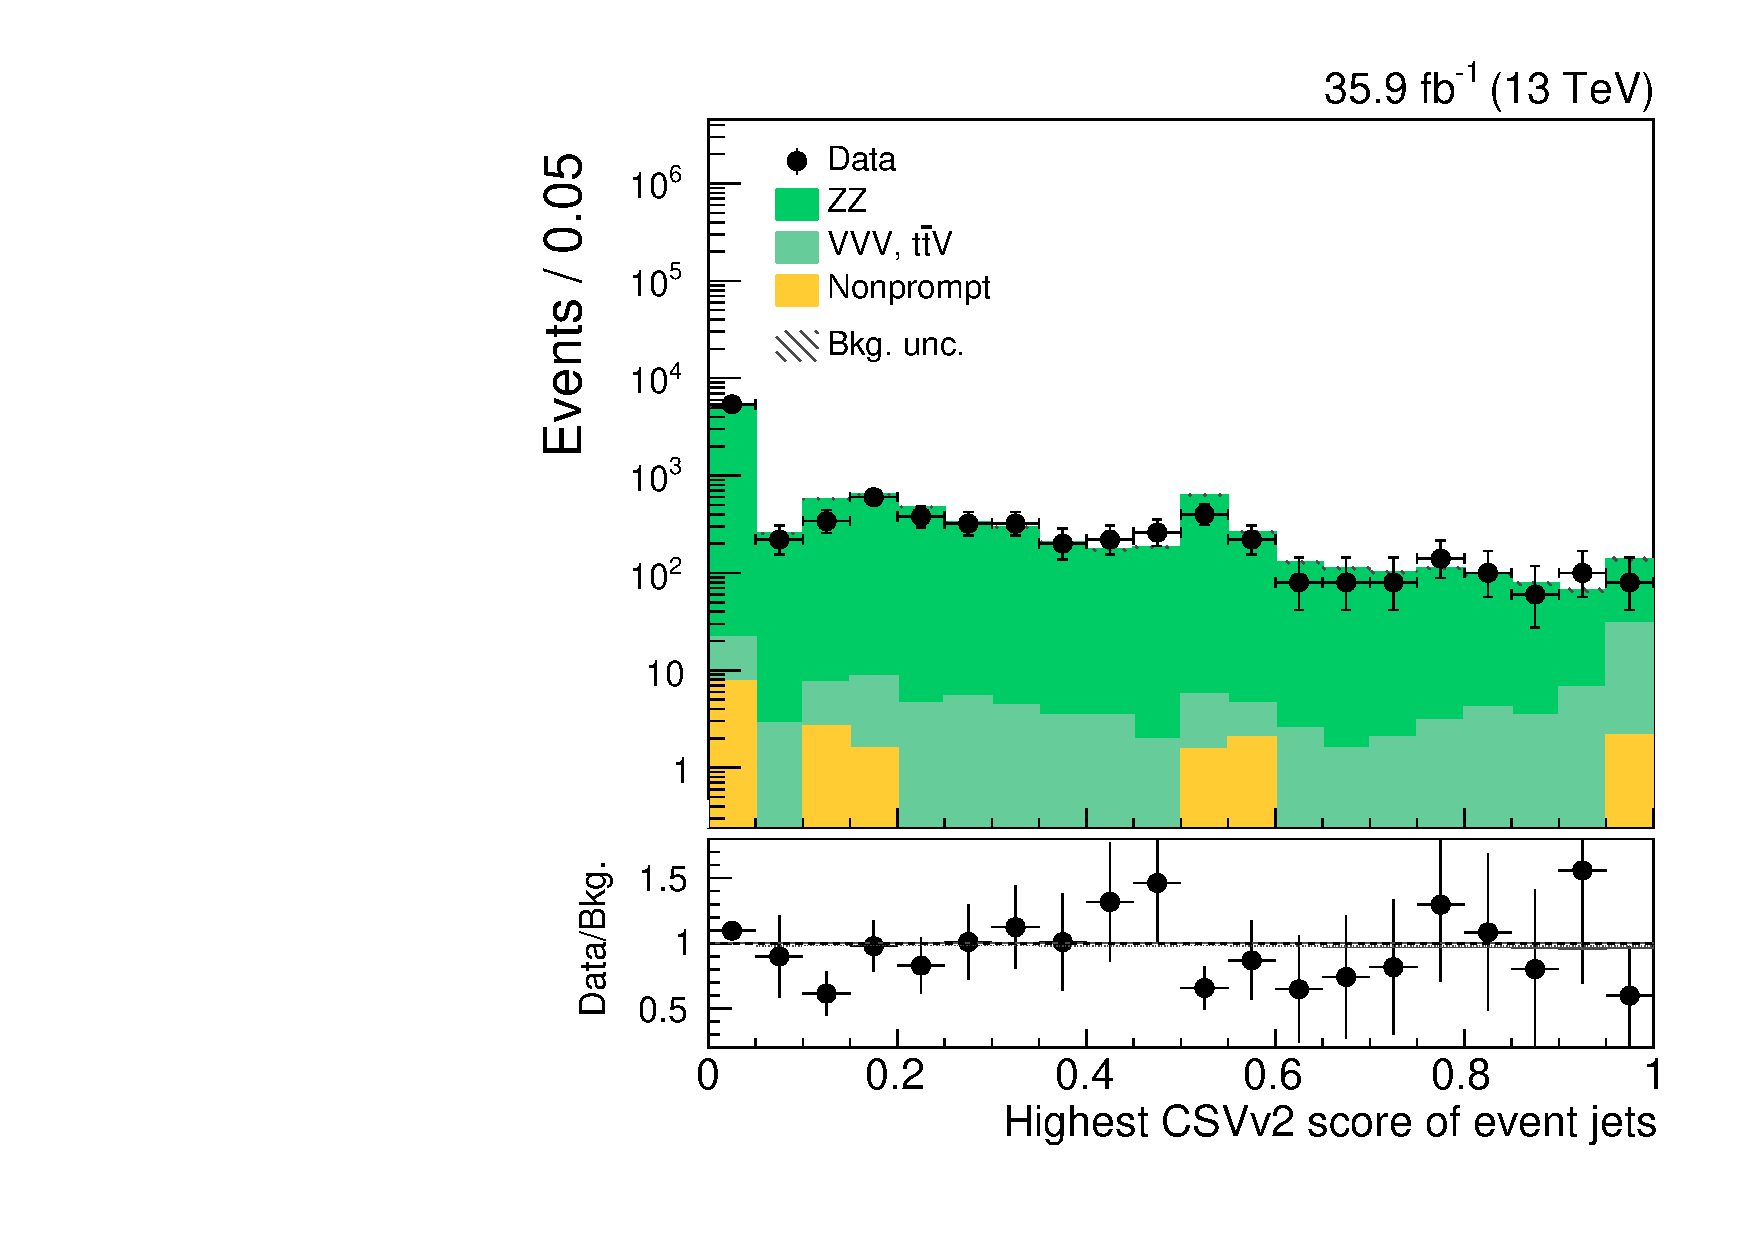
\includegraphics[width=0.48\textwidth]{figures/dibosons/zz4l/bDiscrMax.pdf}
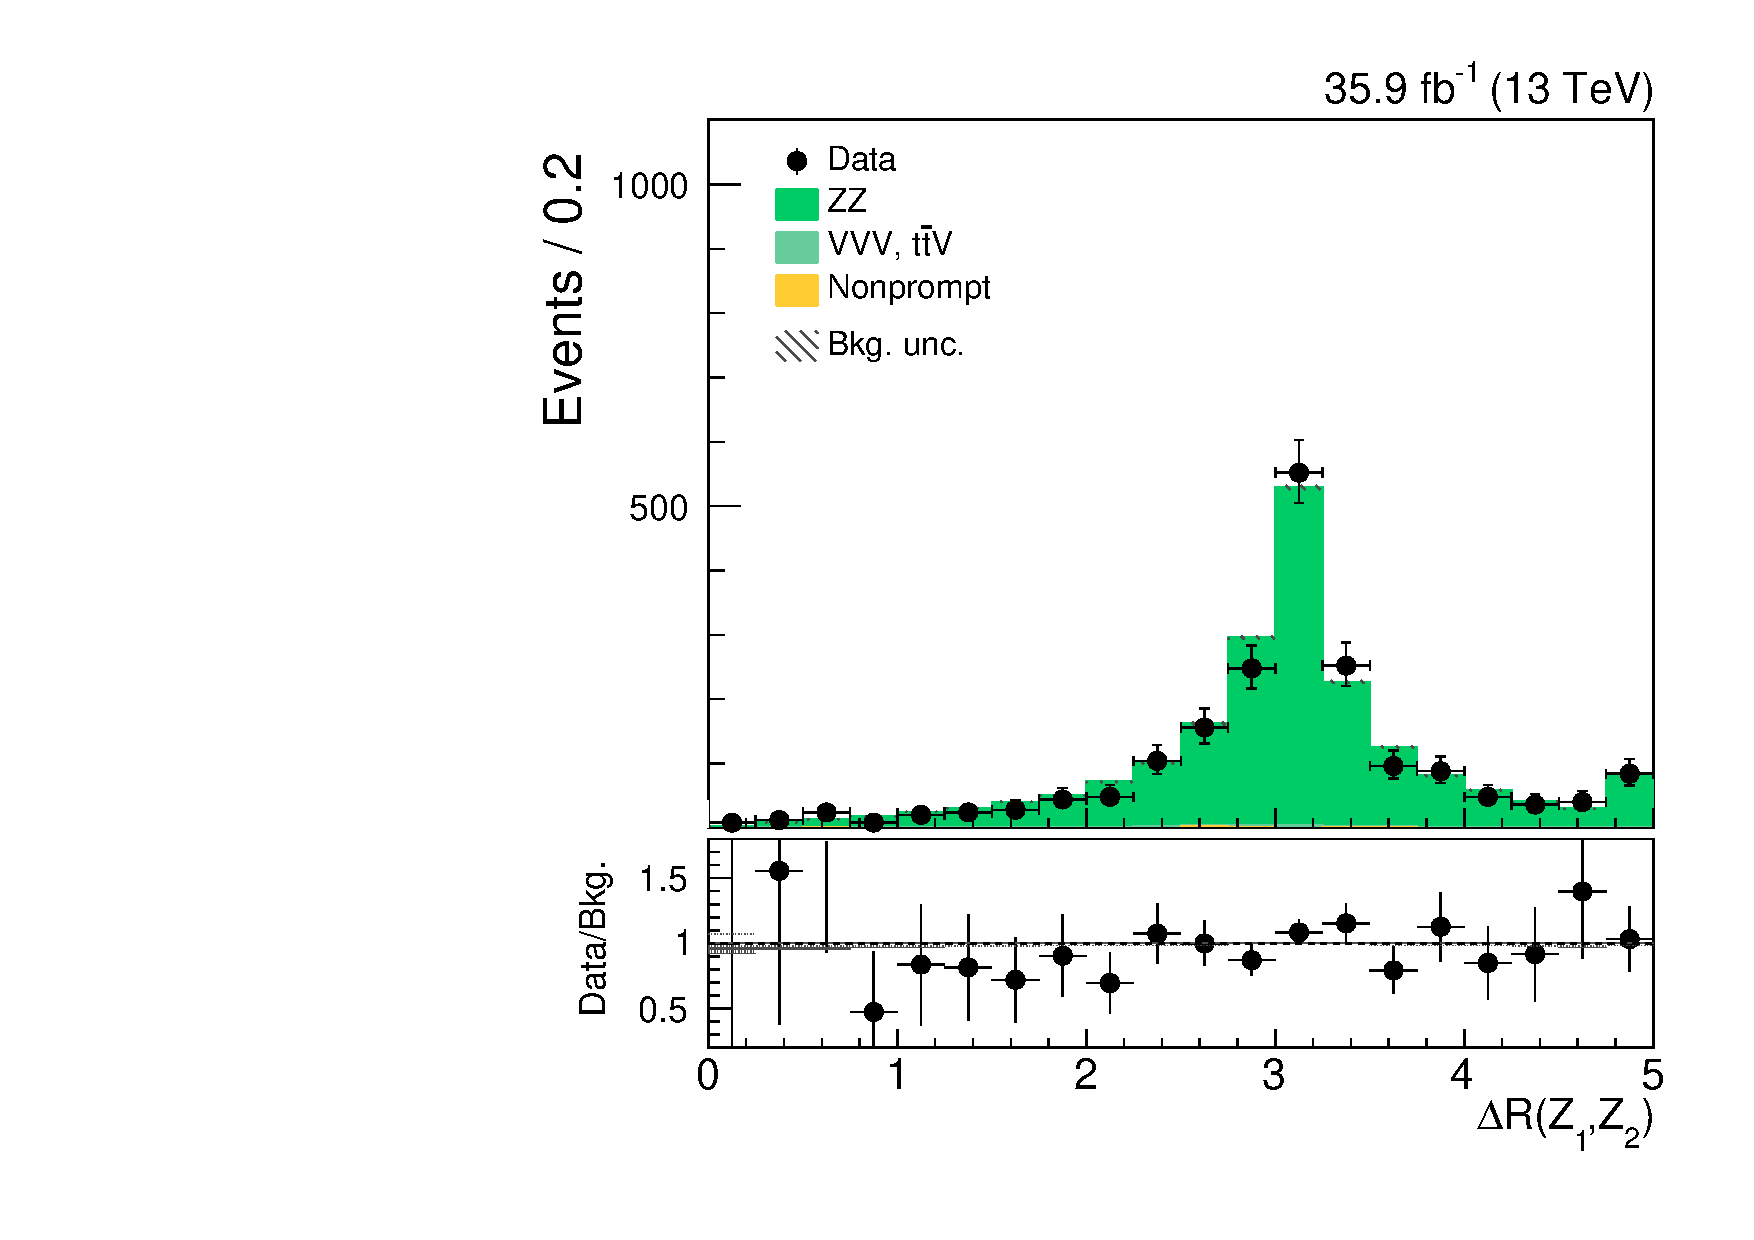
\includegraphics[width=0.48\textwidth]{figures/dibosons/zz4l/dRZ1Z2.pdf}
\caption{More plots of the ZZ data sample.
Clockwise from upper left: diboson invariant mass; azimuthal separation between bosons; the maximum b-tag score of any jet in the event; angular separation between bosons.
The last bin includes the overflow events.
\label{fig:zz4l_moreplots}}
\end{figure}

\clearpage
\begin{figure}[!htb]
\centering
\setlength{\fboxsep}{0pt}
\setlength{\fboxrule}{0.3pt}
\fbox{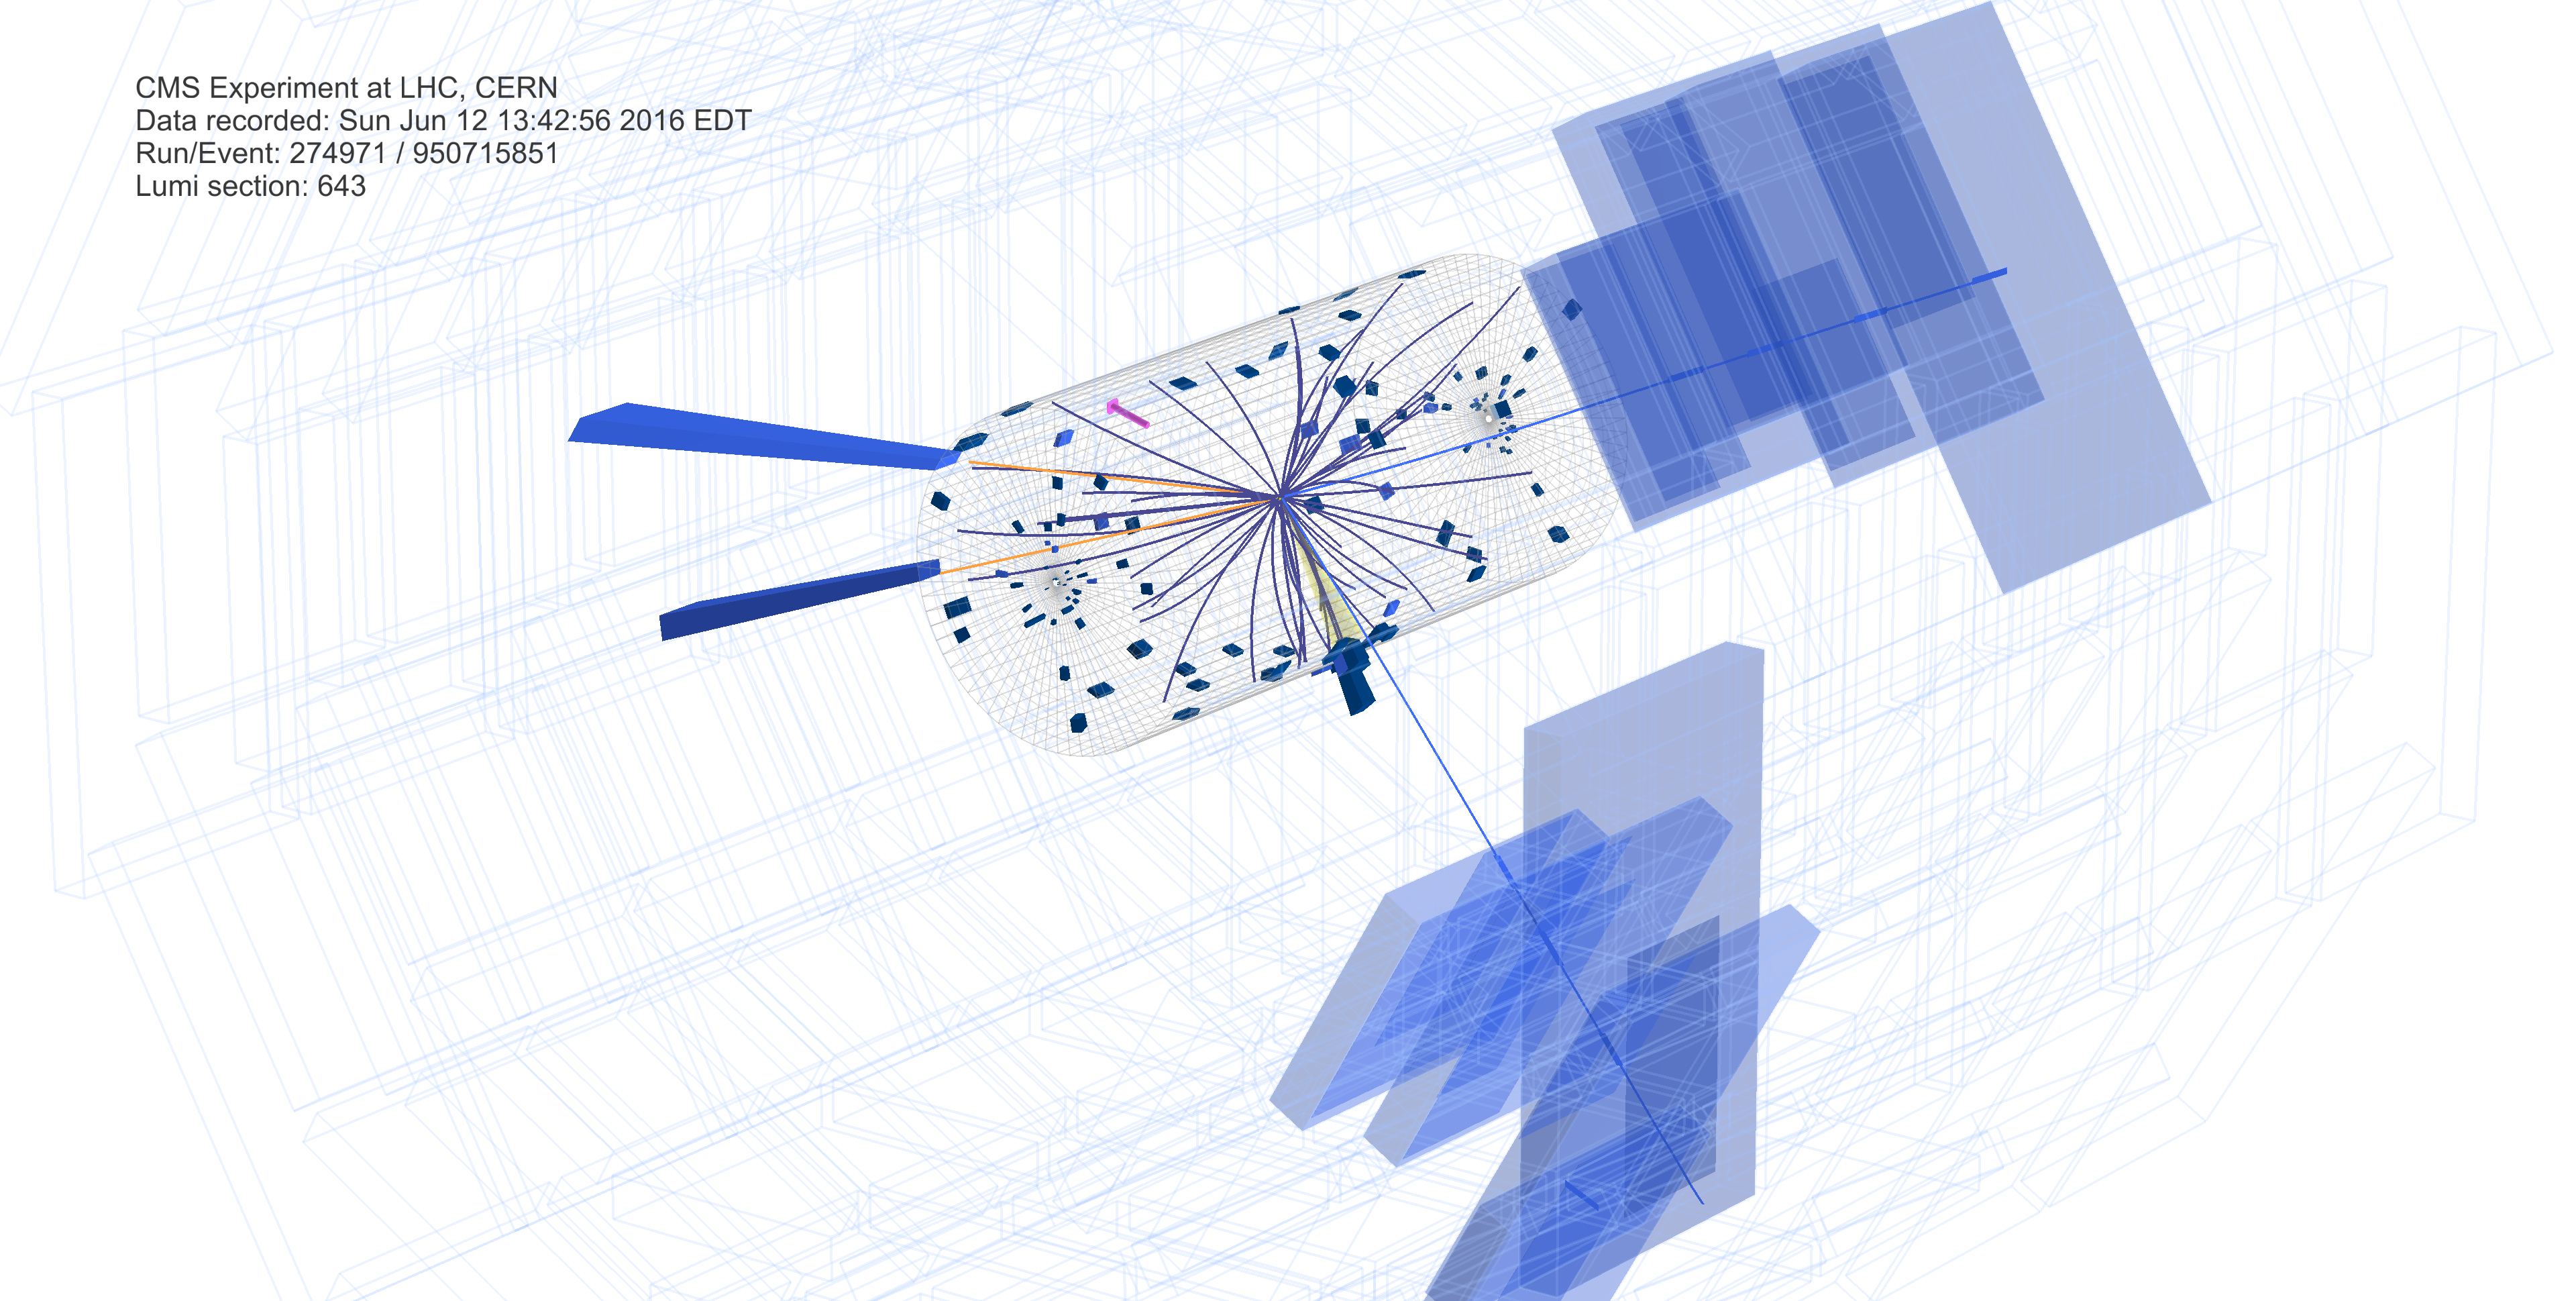
\includegraphics[width=1.0\textwidth]{figures/cmsShow_ZeeZmm_ZpT200-274971_950715851_643_3DTower.png}}\vspace{1cm}

\fbox{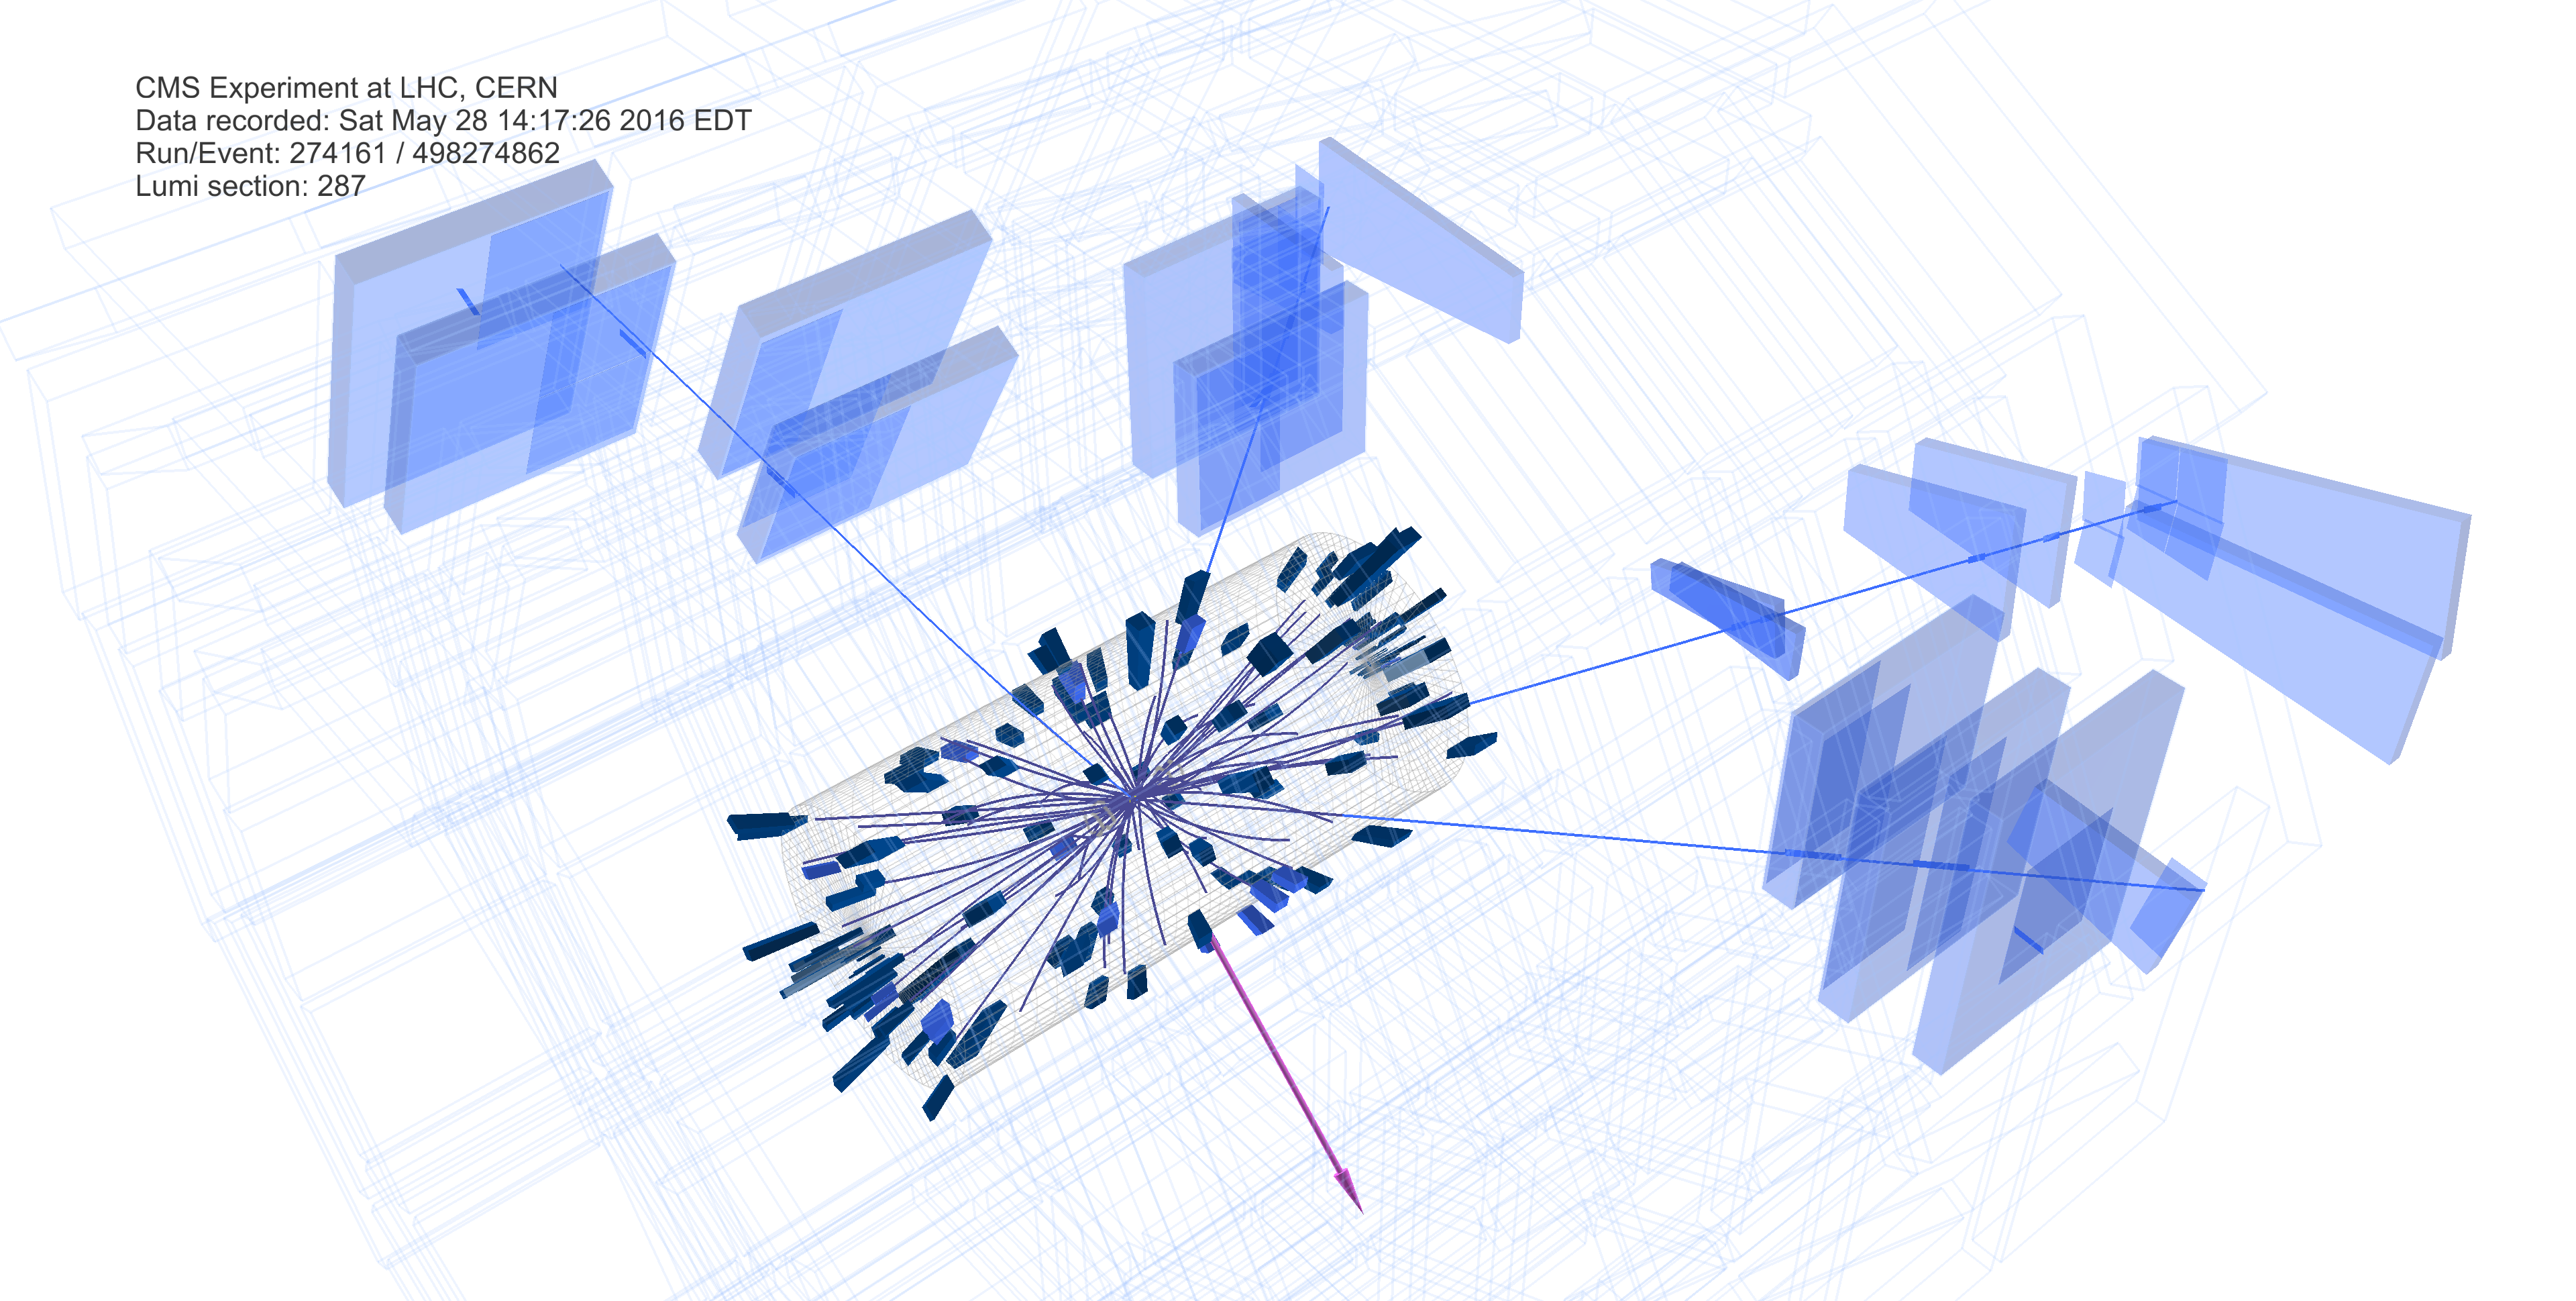
\includegraphics[width=1.0\textwidth]{figures/cmsShow_ZmmZmm_ZpT200-274161_498274862_287_3DTower.png}}\vspace{1cm}

\caption{3D event displays of ZZ($4\ell$) events with Z $p_\mathrm{T} > 200 \GeV$. 
\eventDisplayCaption
\label{fig:zz4l_eventdisplay}}
\end{figure}
\clearpage


\section{Visible WZ process}
\label{sec:wz3l}
Next, I will describe how events are selected to observe fully visible WZ production. 
The events must have three well-reconstructed leptons and a nominal amount of $\met$.
A single Z boson candidate is formed from a pair of opposite-charge electrons or muons having invariant mass within 15 \GeV of the Z boson mass.
Additionally, a third well-identified electron or muon is required, representing the W boson.
In the case where there are three electrons or muons,
the Z candidate is chosen unambiguously as the opposite-sign pair whose invariant mass is closest to the Z boson mass.

True WZ events are expected to have an undetectable neutrino in the final state, thus $\met$ of at least 30\GeV is required.
To exclude a region where production of Z bosons with final-state radiation may contribute, the trilepton invariant mass is required to be more than 100 \GeV.
Due to theoretical problems with collinear emission of same-flavor opposite-sign dilepton pairs, the invariant mass of any opposite-sign lepton pair ($m_{2\Lep}$) is required to be larger than $4\GeV$.
These requirements follow precedent for the measurement of the $\WZ$ production cross section with CMS~\cite{Khachatryan:2016tgp}.

Since there is no danger of contamination, no veto on additional hadronically-decaying $\tau$ leptons is applied.
A relaxed b-jet veto is applied which rejects events where a jet passes the most stringent b-jet identification requirement.
This, along with the Z candidate invariant mass requirement, is useful for rejecting ditop background.

The selection yields in simulation and data for the WZ analysis are shown in Table~\ref{tab:wz3lyields}.
Kinematic variables of the bosons, and variables used in the selection, are shown in Figures~\ref{fig:wz3l_z},~\ref{fig:wz3l_purity}, and~\ref{fig:wz3l_w}.
In particular, note the presence of the expected Jacobian peak in the W boson transverse mass distribution in Figure~\ref{fig:wz3l_w}.
The transverse mass is calculated in the transverse $(r,\phi)$ plane using the 
third lepton ($\vec{\mathbf{p}}_\mathrm{T}^\ell$) and missing energy ($\vec{\mathbf{p}}_\mathrm{T}^\mathrm{miss}$) vectors:
\begin{equation}
\label{eq:mt}
\begin{split}
m_\mathrm{T} & = \sqrt{m_\ell^2 + m_\nu^2 + 2(E_\ell E_\nu -\vec{\mathbf{p}}_\mathrm{T}^\ell \cdot \vec{\mathbf{p}}_\mathrm{T}^\mathrm{miss})} \\ 
& \approx \sqrt{2\:|\vec{\mathbf{p}}_\mathrm{T}^\ell|\:|\vec{\mathbf{p}}_\mathrm{T}^\mathrm{miss}|\:(1 - \mathrm{cos}\:\Delta\phi)} \qquad \mathrm{for}\:m_\ell,\:m_\nu\approx0
\end{split}
\end{equation}
where $\Delta\phi$ is the azimuthal separation between those vectors.

\clearpage
\begin{figure}[!t]
\centering
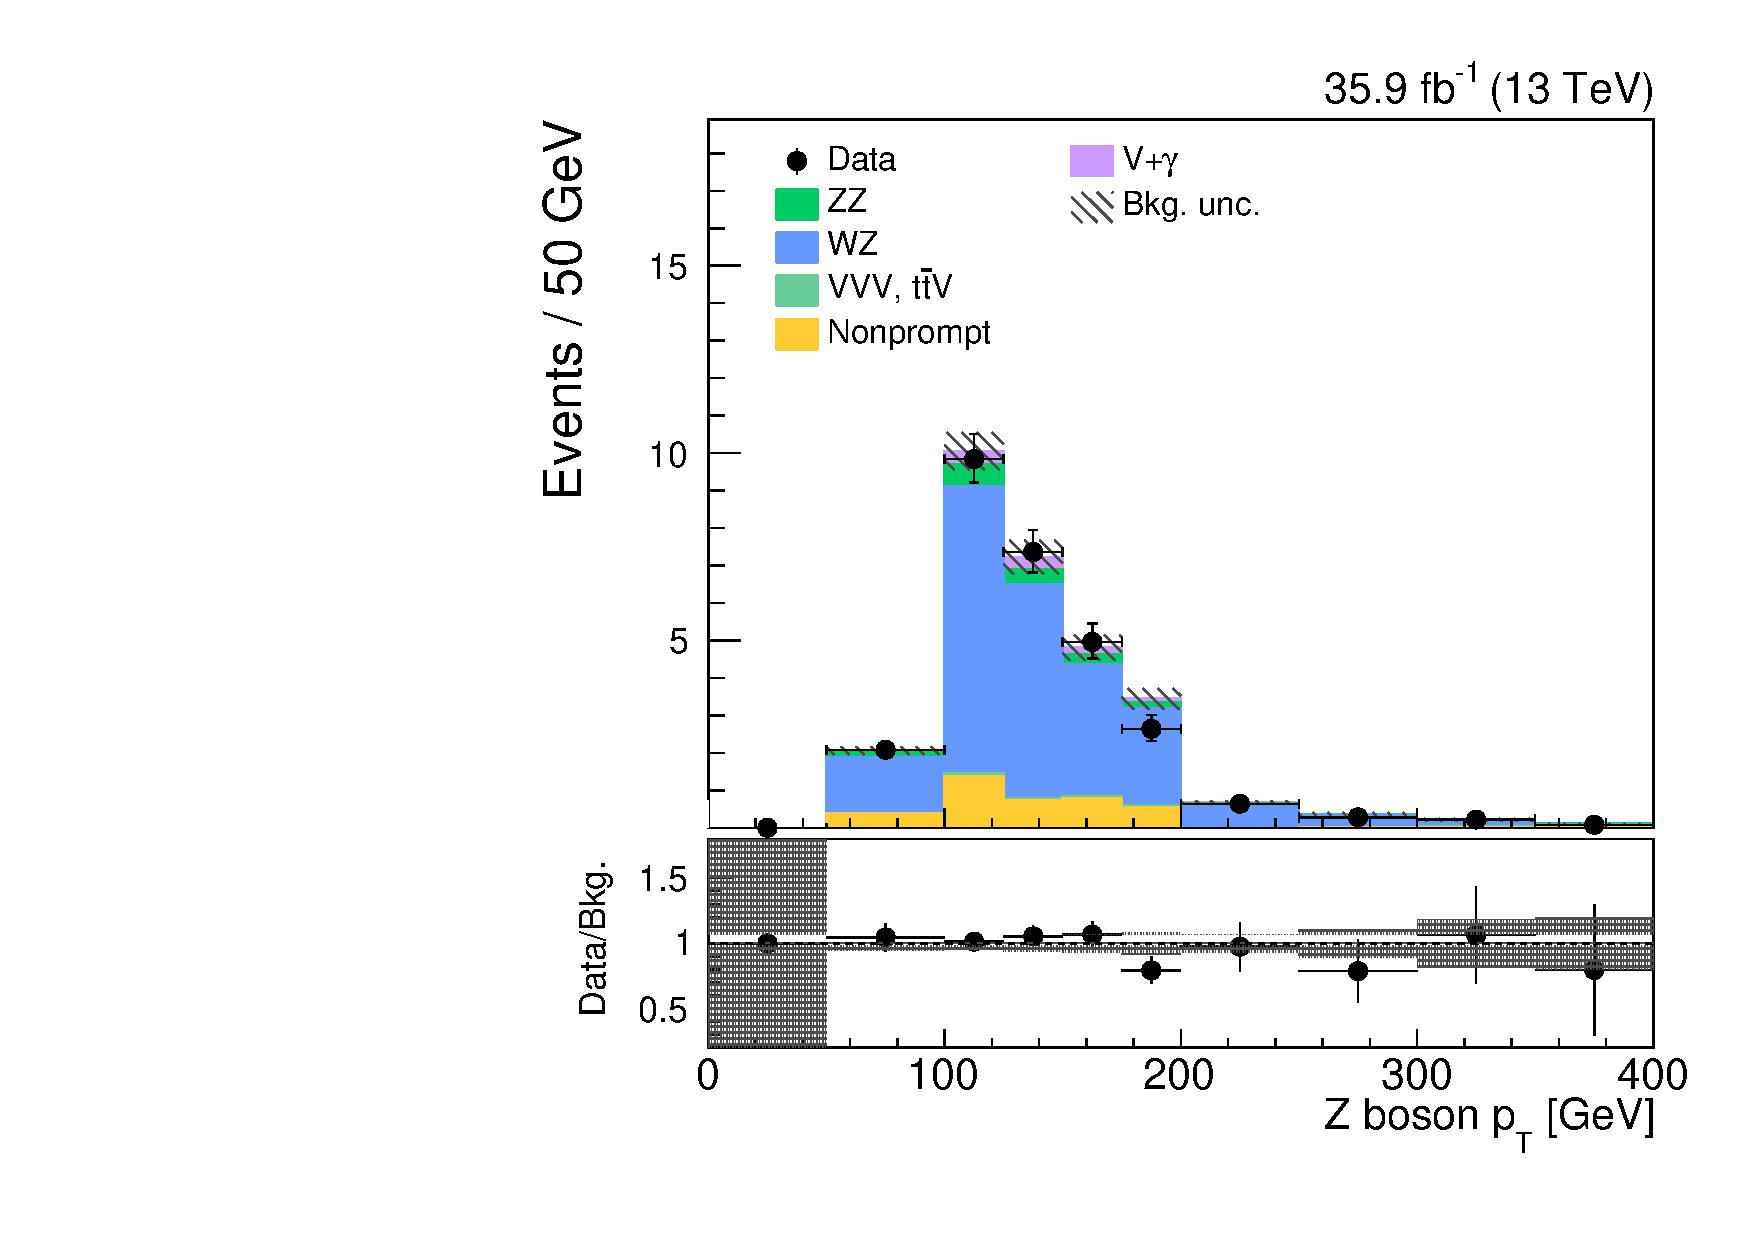
\includegraphics[width=0.48\textwidth]{figures/dibosons/wz3l/pTZ.pdf}
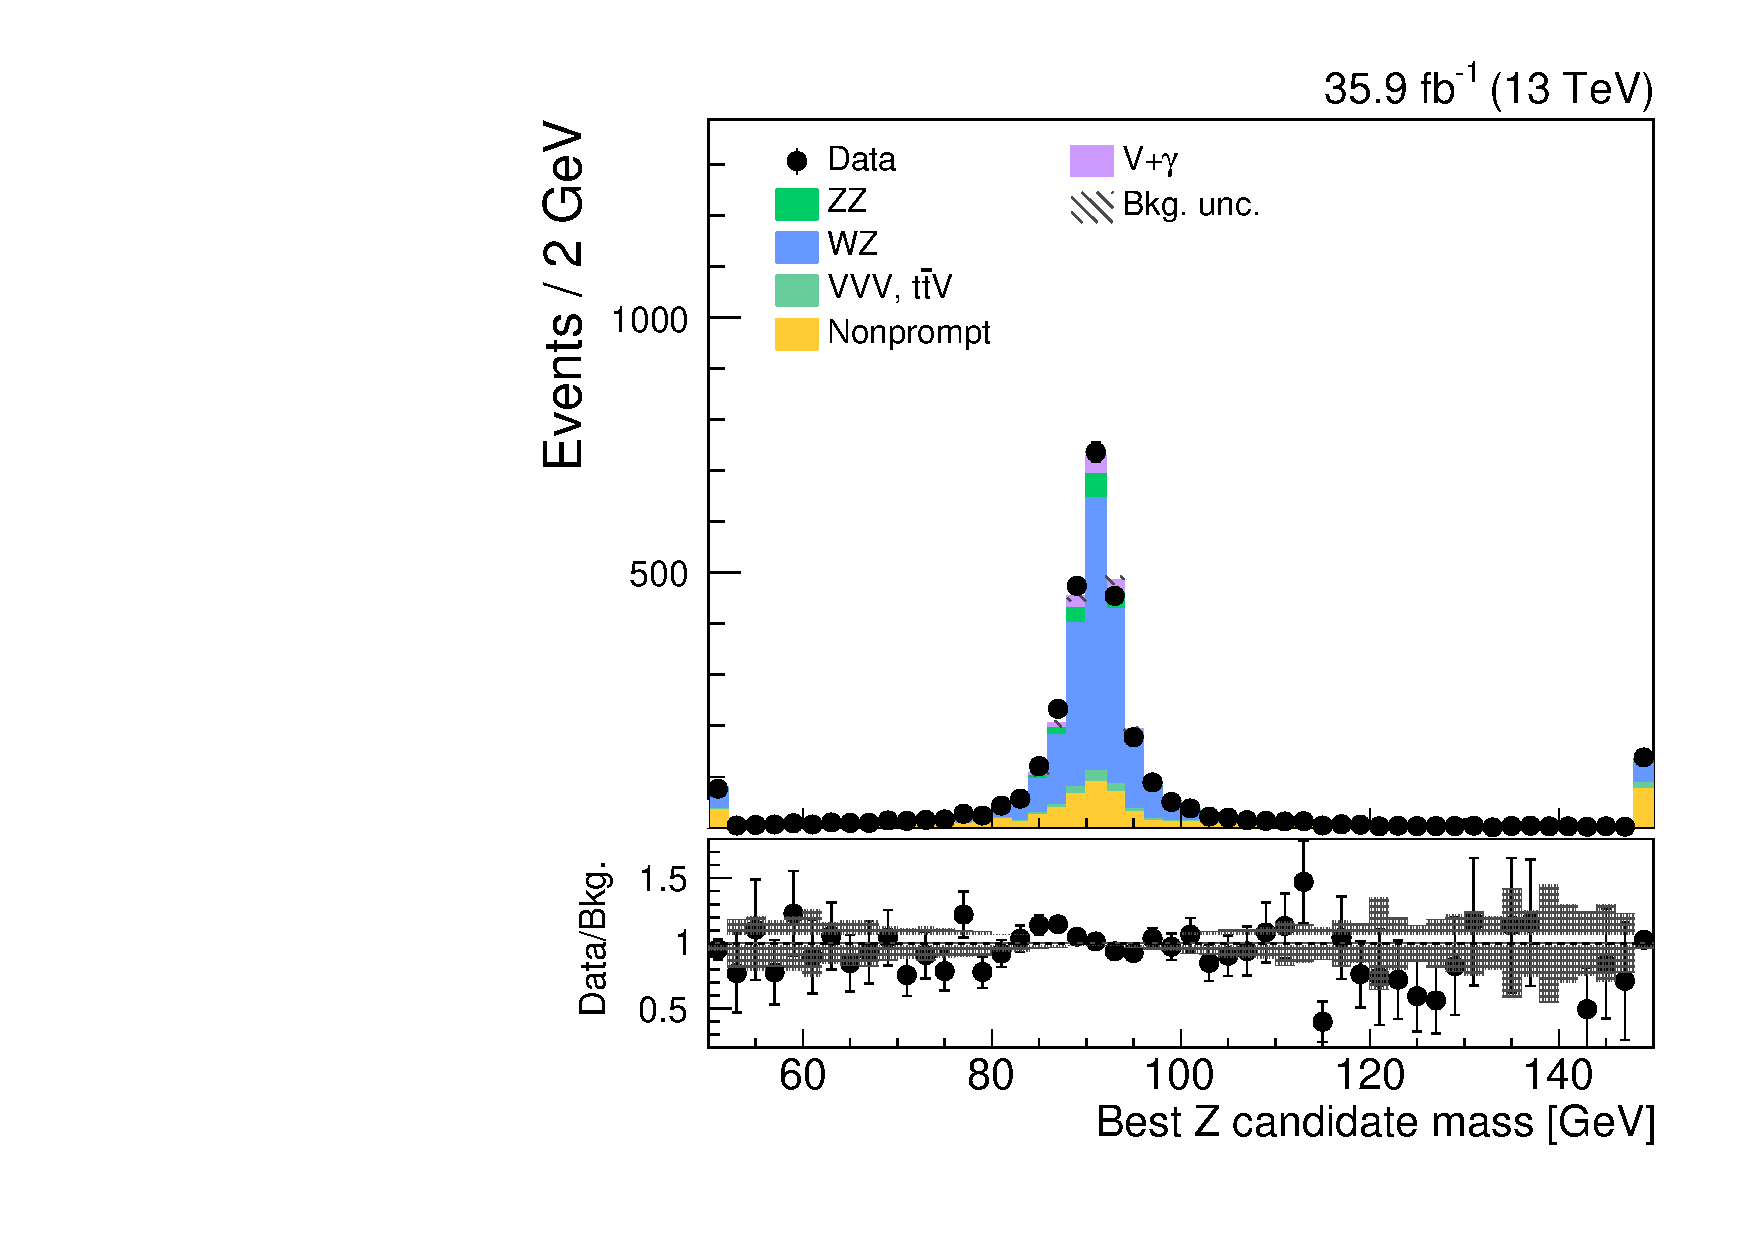
\includegraphics[width=0.48\textwidth]{figures/dibosons/wz3l/minMassZ_Nminus1.pdf}
\caption{The transverse momentum and invariant mass of the reconstructed Z boson candidate.
The last bin includes the overflow events.
\label{fig:wz3l_z}}
\end{figure}

\begin{figure}[!hb]
\centering
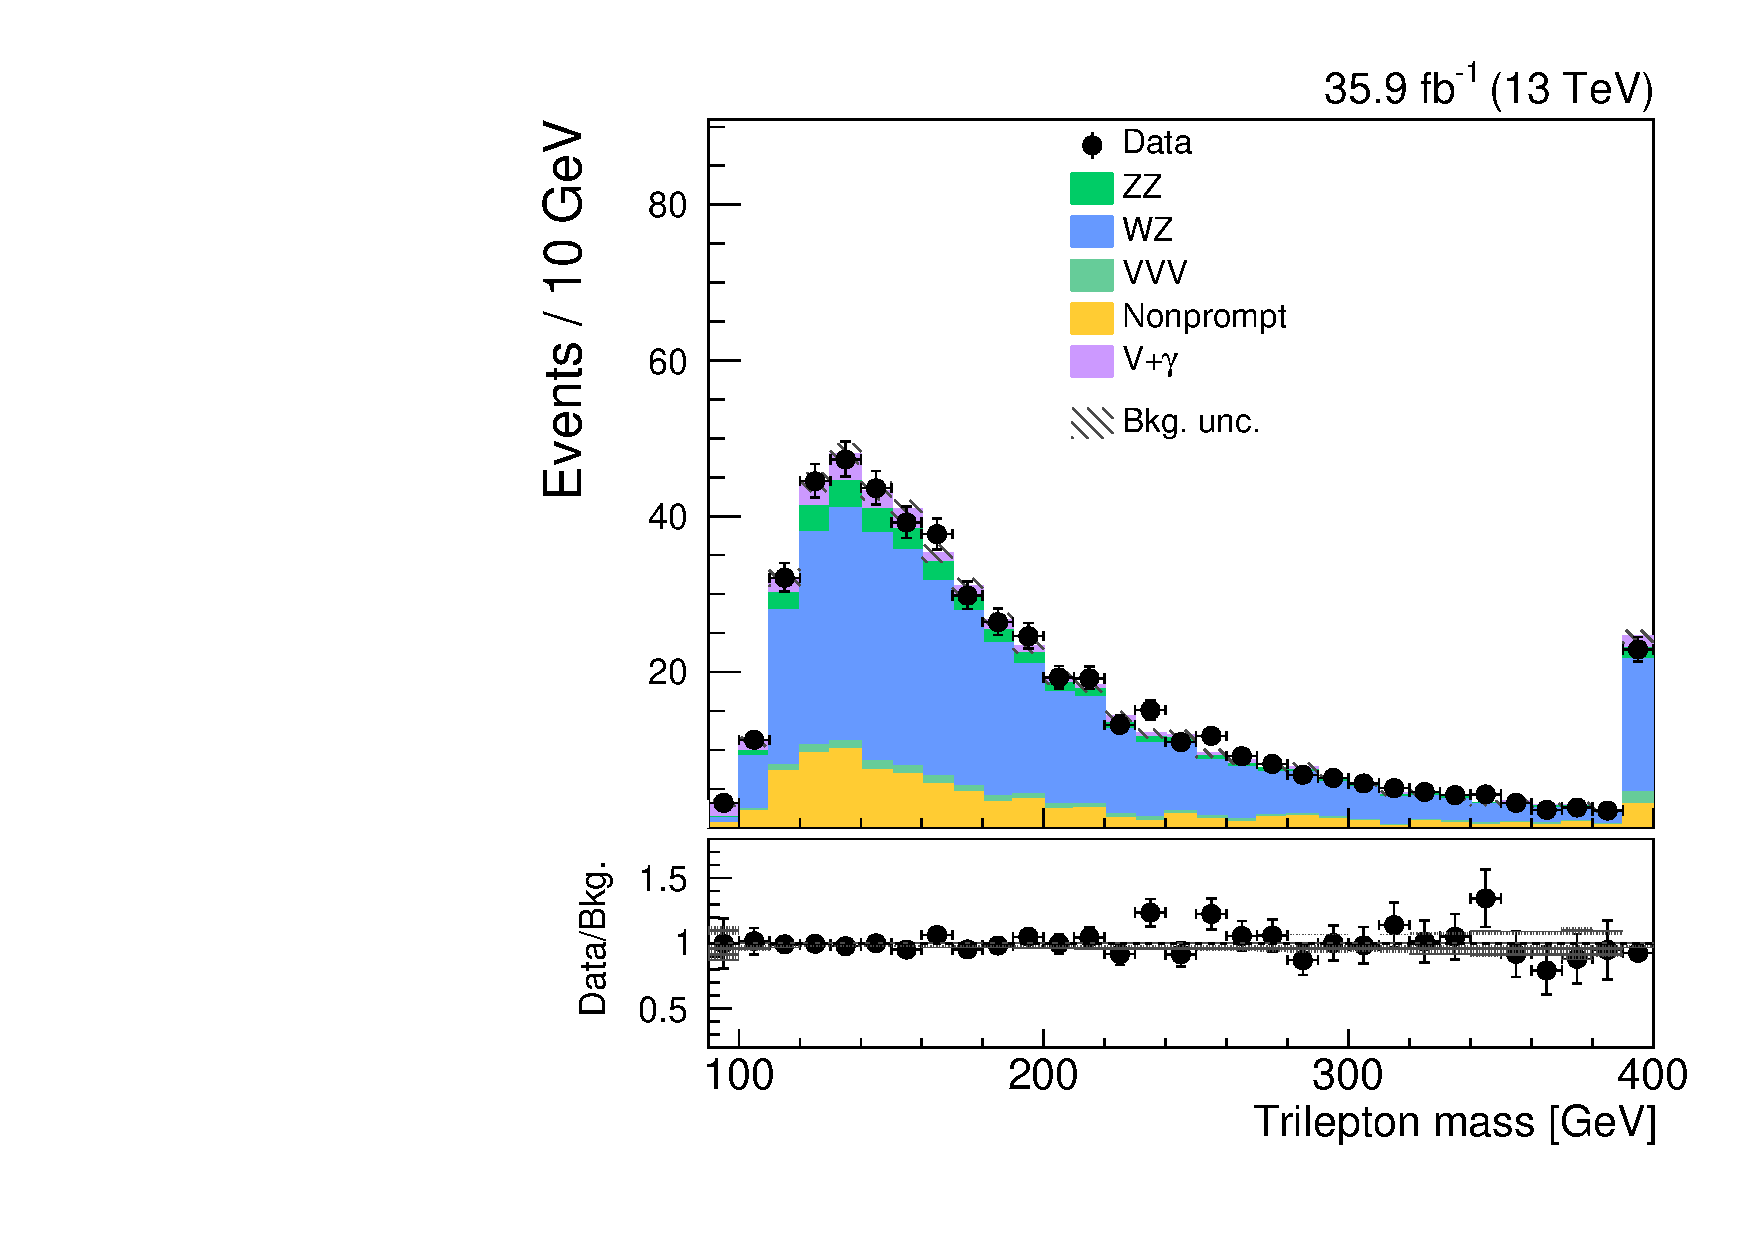
\includegraphics[width=0.48\textwidth]{figures/dibosons/wz3l/m3l_Nminus1.pdf}
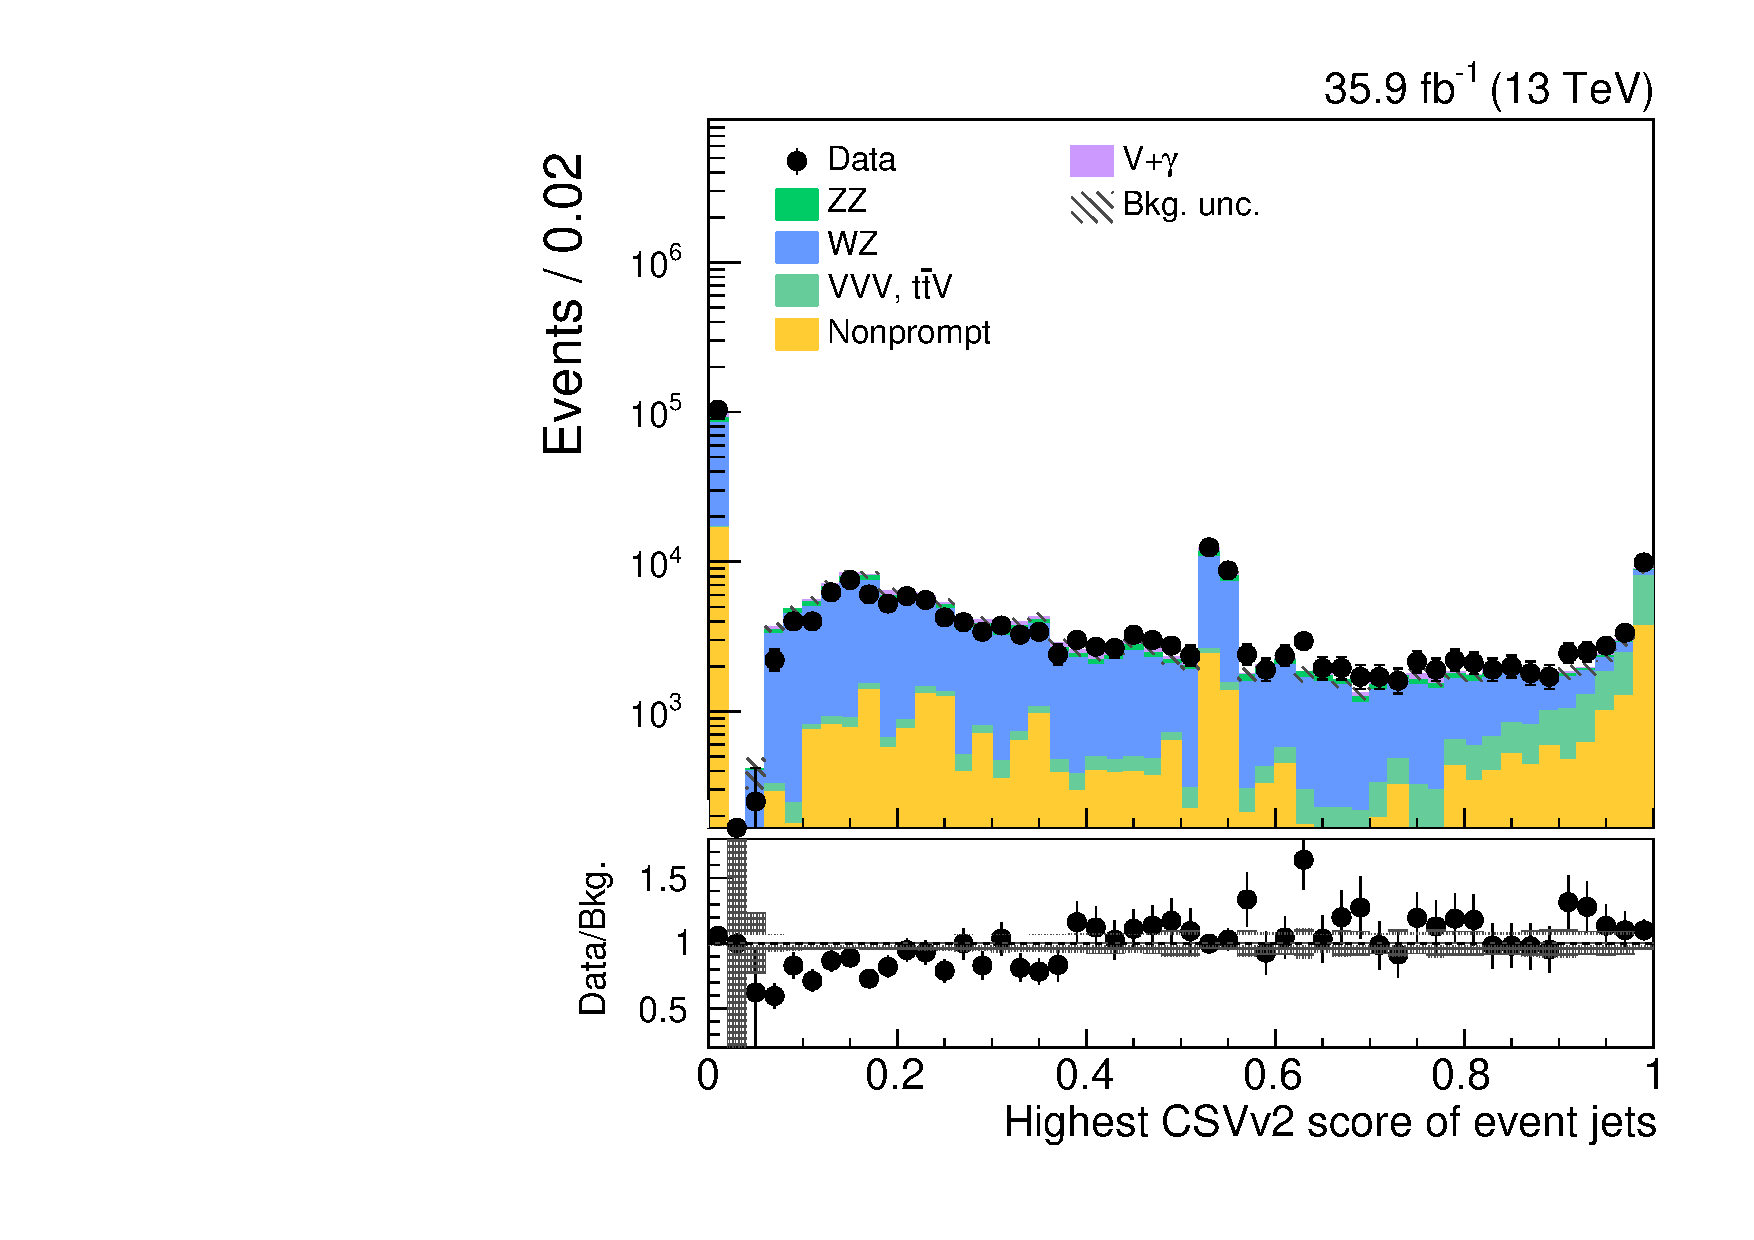
\includegraphics[width=0.48\textwidth]{figures/dibosons/wz3l/bDiscrMax_Nminus1.pdf}
\caption{Trilepton invariant mass and the maximum b-tag score of any jet in the event
at final selection level.
The last bin includes the overflow events.
Events with a well b-tagged jet ($>0.9535$) are rejected--note the low purity in the last few bins.
\label{fig:wz3l_purity}}
\end{figure}

\clearpage

\begin{figure}[!th]
\centering
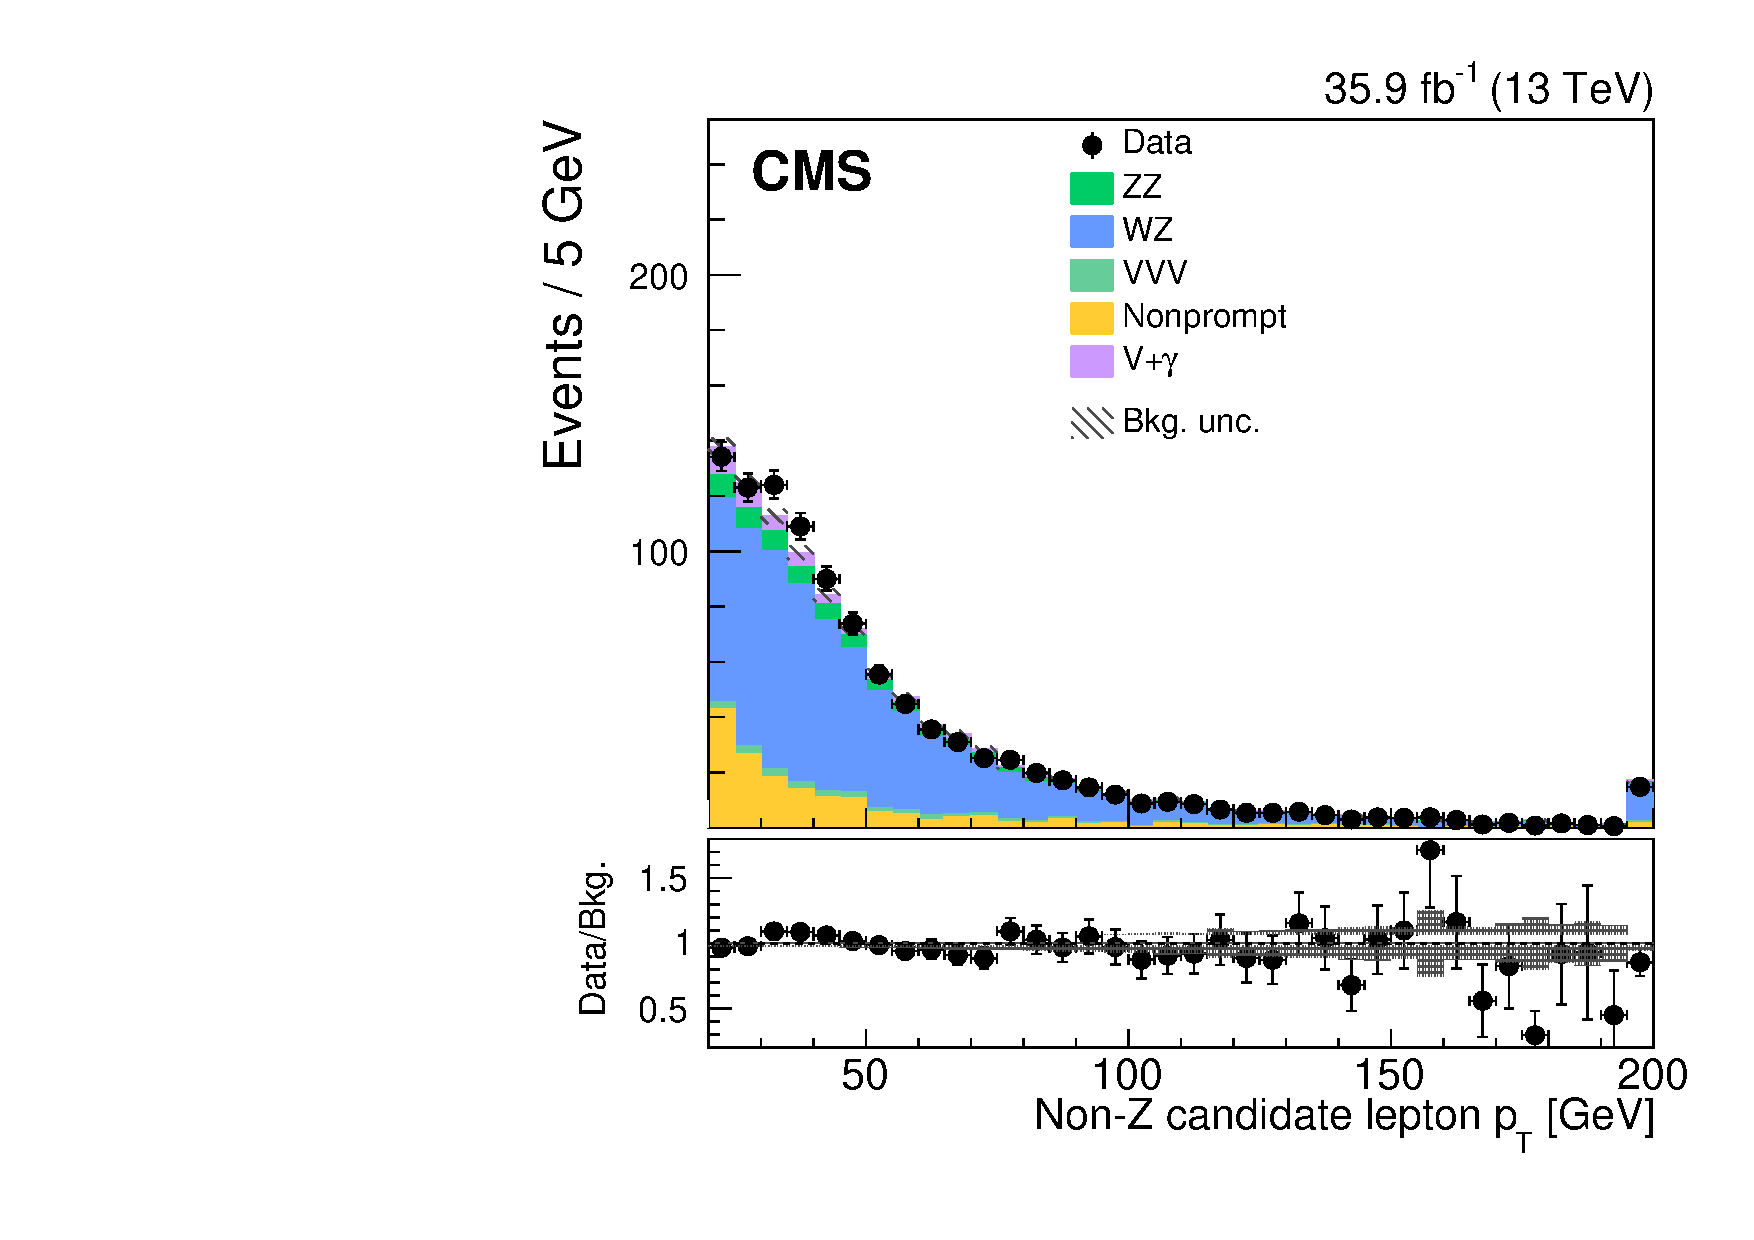
\includegraphics[width=0.48\textwidth]{figures/dibosons/wz3l/lepWpT_Nminus1.pdf}
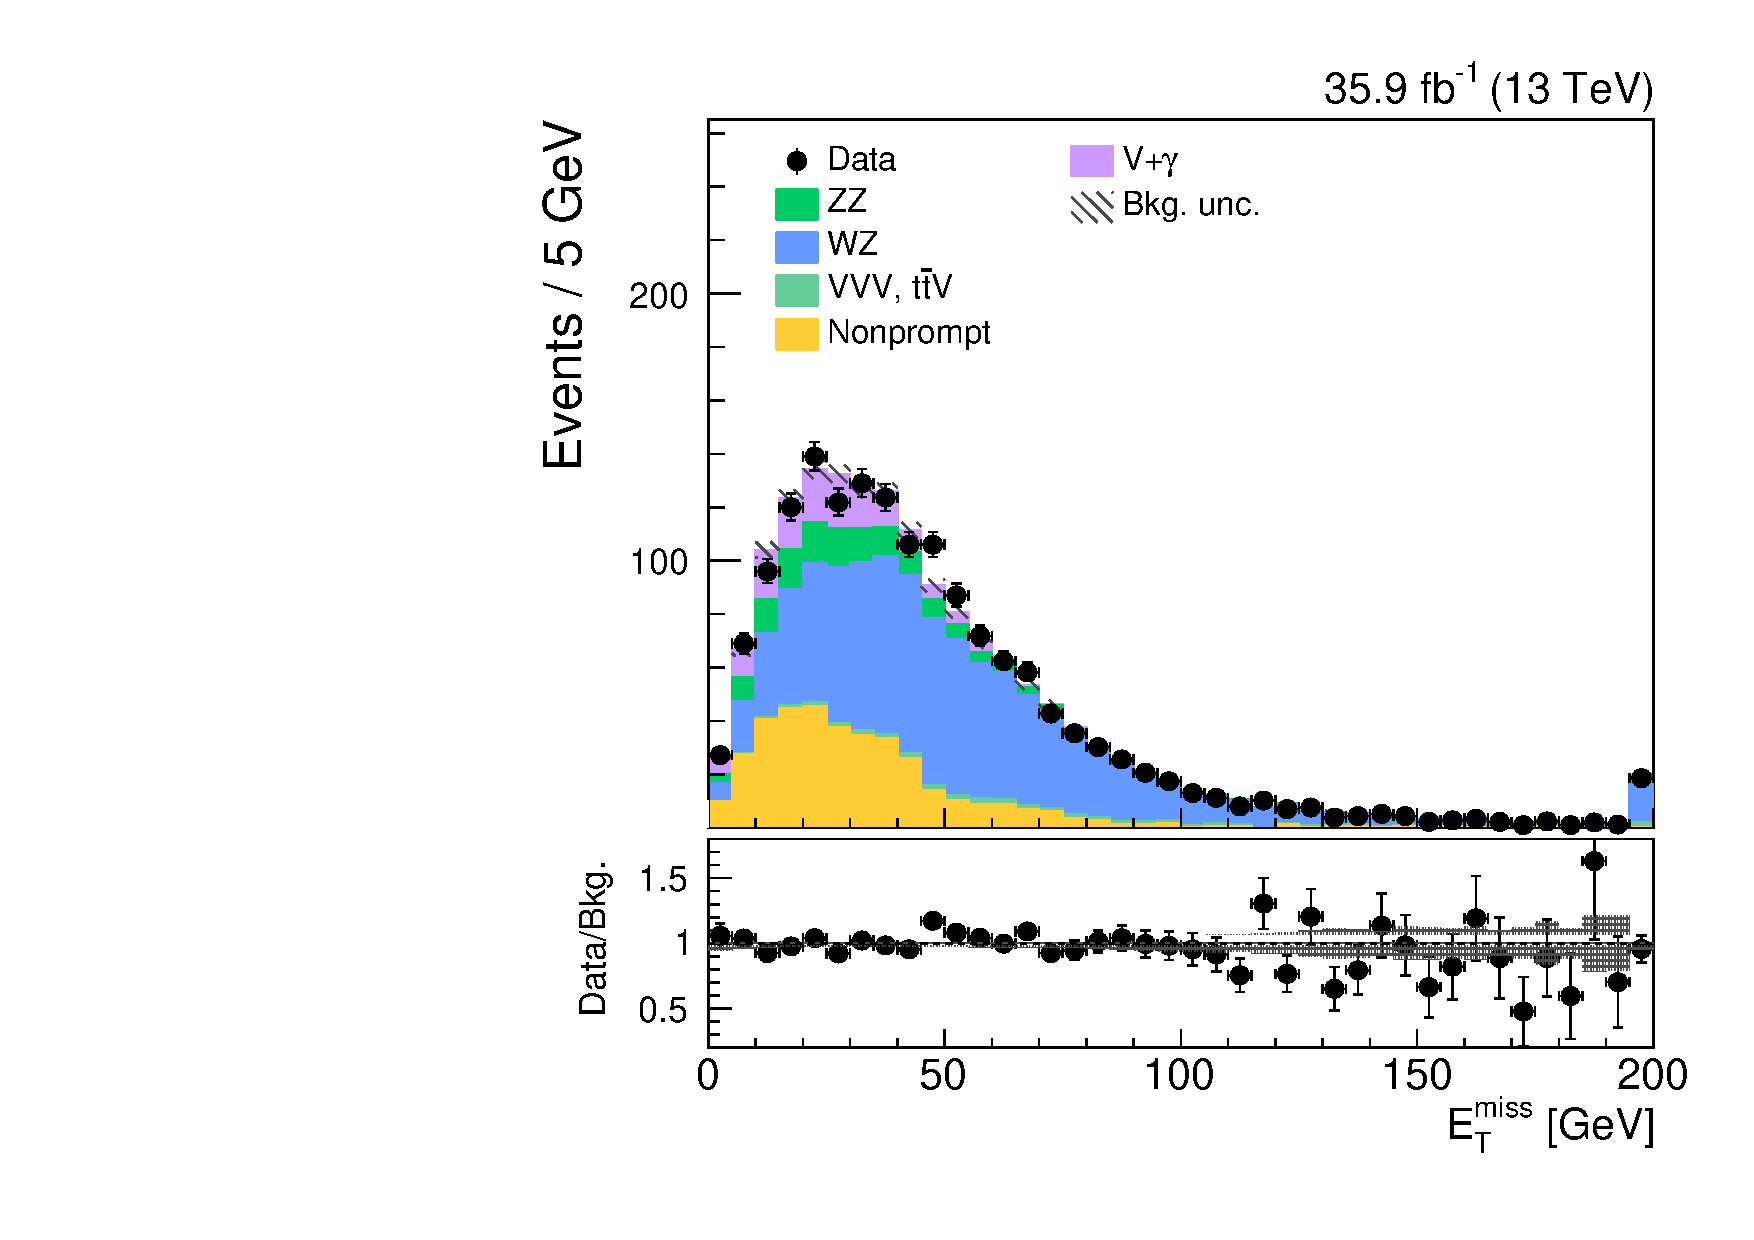
\includegraphics[width=0.48\textwidth]{figures/dibosons/wz3l/met_Nminus1.pdf}
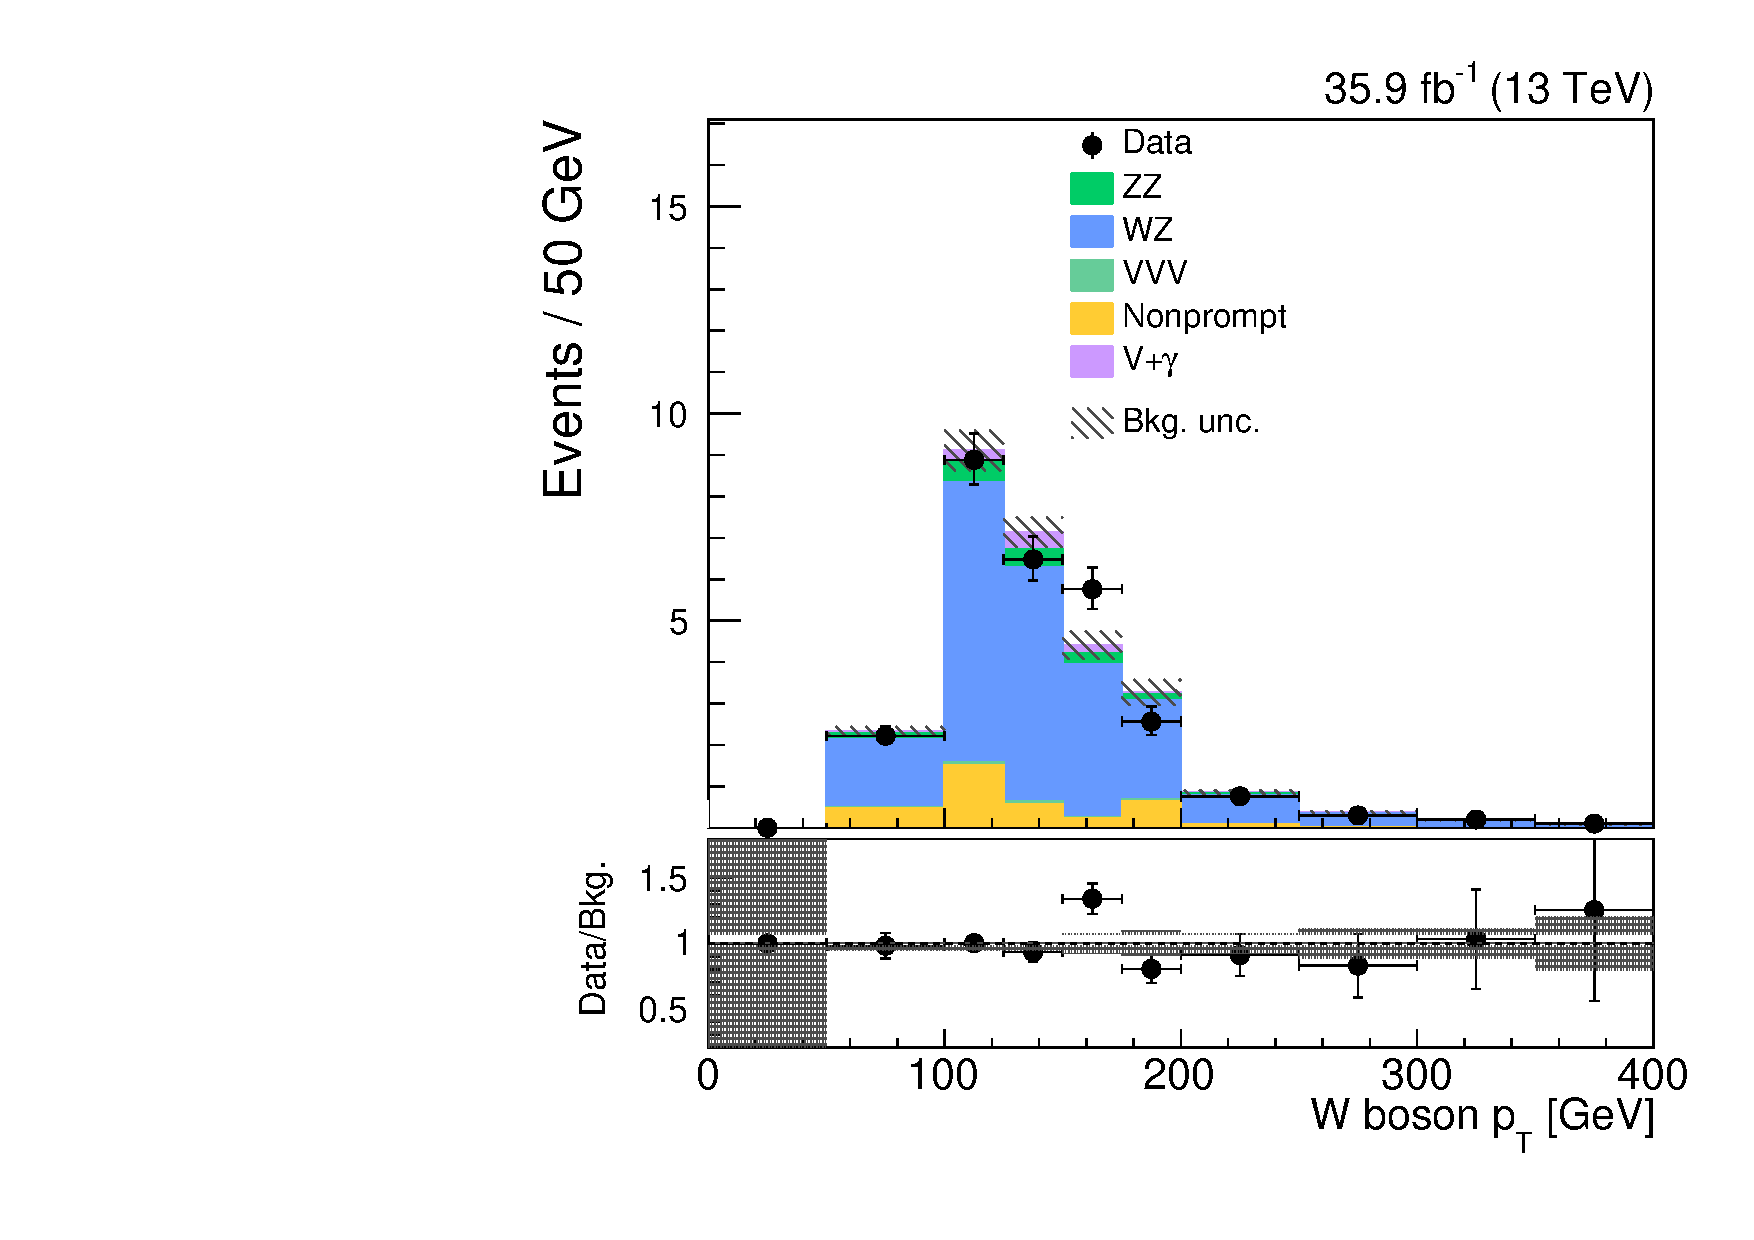
\includegraphics[width=0.48\textwidth]{figures/dibosons/wz3l/pTW.pdf}
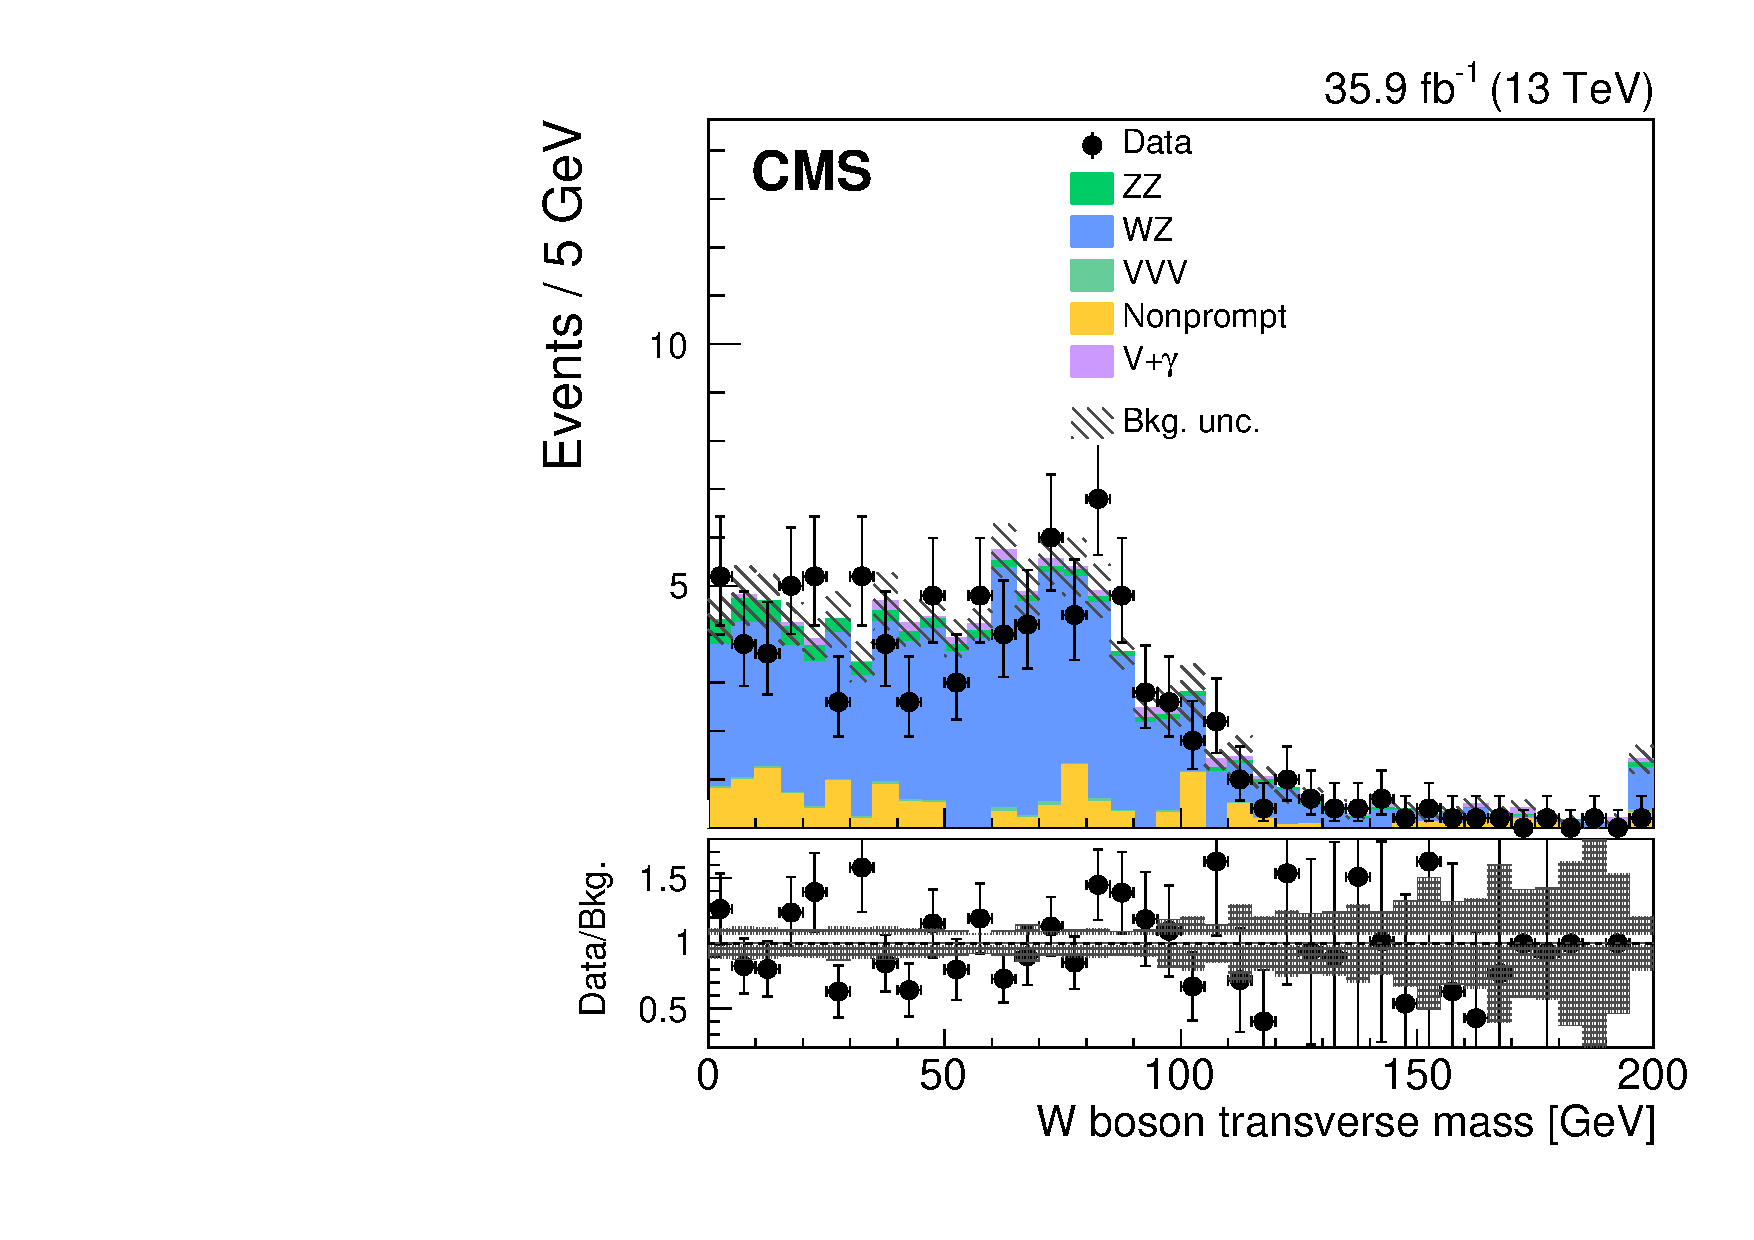
\includegraphics[width=0.48\textwidth]{figures/dibosons/wz3l/mTW.pdf}
\caption{Kinematics of the reconstructed W boson at final selection level. Clockwise from upper left: 
$p_\mathrm{T}$ of the lepton associated with the W boson;
$\met$ in the event; transverse mass of the W boson;
and $p_\mathrm{T}$ of the W boson.
Note the Jacobian peak in the transverse mass distribution.
The last bin includes the overflow events.
\label{fig:wz3l_w}}
\end{figure}

%Selection: WZSEL
%(....WZ):   117.14 +/-   3.12 |    89.52 +/-   2.71 |    89.52 +/-   2.71 |    67.29 +/-   2.33 | 363.48 +/-   5.47
%(....EM):    11.00 +/-   2.46 |    25.34 +/-   7.12 |    12.27 +/-   3.07 |    16.33 +/-   6.20 |  64.94 +/-  10.23
%( ...ZZ):     9.42 +/-   0.24 |     7.04 +/-   0.21 |     6.99 +/-   0.20 |     4.56 +/-   0.16 |  28.00 +/-   0.41
%(...VVV):     1.69 +/-   0.18 |     1.14 +/-   0.15 |     1.23 +/-   0.16 |     0.98 +/-   0.16 |   5.04 +/-   0.32
%(Zgamma):     0.36 +/-   0.36 |     0.03 +/-   0.52 |     8.28 +/-   2.14 |     6.87 +/-   1.83 |  15.54 +/-   2.88
%(...bkg):   139.61 +/-   4.07 |   123.06 +/-   7.67 |   118.30 +/-   4.67 |    96.03 +/-   6.90 | 477.00 +/-  12.03
%(..Data):   146.00 +/-  12.08 |   112.00 +/-  10.58 |   111.00 +/-  10.54 |   108.00 +/-  10.39 | 477.00 +/-  21.84
%-----------------------------------------------------------------------------------------------------------
\setlength{\tabcolsep}{12pt}
\begin{table}[!b]
  \caption{Predicted and observed number of events for the WZ three-lepton selection using $\usedLumi$.
  Only statistical uncertainties are reported.
  \label{tab:wz3lyields}}
  \begin{center}
{\scriptsize
  \begin{tabular}{rlllll}
\hline 
Process & $\mathrm{W}(\mu\nu)\mathrm{Z}(\mu\mu)$ & $\mathrm{W}(\mu\nu)\mathrm{Z}(ee)$ & $\mathrm{W}(e\nu)\mathrm{Z}(\mu\mu)$ & $\mathrm{W}(e\nu)\mathrm{Z}(ee)$ & Total \\
\hline
WZ                    &  117.1 $\pm$ 3.1 &   89.5 $\pm$  2.7 &   89.5 $\pm$ 2.7 &  67.3 $\pm$ 2.3 & 363.5 $\pm$   5.5 \\ 
Nonprompt bkg.        &   11.0 $\pm$ 2.5 &   25.3 $\pm$  7.1 &   12.3 $\pm$ 3.1 &  16.3 $\pm$ 6.2 &  64.9 $\pm$  10.2 \\ 
ZZ                    &    9.4 $\pm$ 0.2 &    7.0 $\pm$  0.2 &    7.0 $\pm$ 0.2 &   4.6 $\pm$ 0.2 &  28.0 $\pm$   0.4 \\ 
VVV                   &    1.7 $\pm$ 0.2 &    1.1 $\pm$  0.2 &    1.2 $\pm$ 0.2 &   1.0 $\pm$ 0.2 &   5.0 $\pm$   0.3 \\ 
V+$\gamma$            &    0.4 $\pm$ 0.4 &    0.0 $\pm$  0.5 &    8.3 $\pm$ 2.1 &   6.9 $\pm$ 1.8 &  15.5 $\pm$   2.9 \\ 
\hline
Total                 &  139.6 $\pm$ 4.1 &  123.1 $\pm$  7.7 &  118.3 $\pm$ 4.7 &  96.0 $\pm$ 6.9 & 477.0 $\pm$  12.0 \\
\hline
Data                  &  146             &  112              &  111             & 108             & 477               \\
\hline
  \end{tabular}
}
  \end{center}
\end{table}

\clearpage
\begin{figure}[!htb]
\centering
\setlength{\fboxsep}{0pt}
\setlength{\fboxrule}{0.3pt}
\fbox{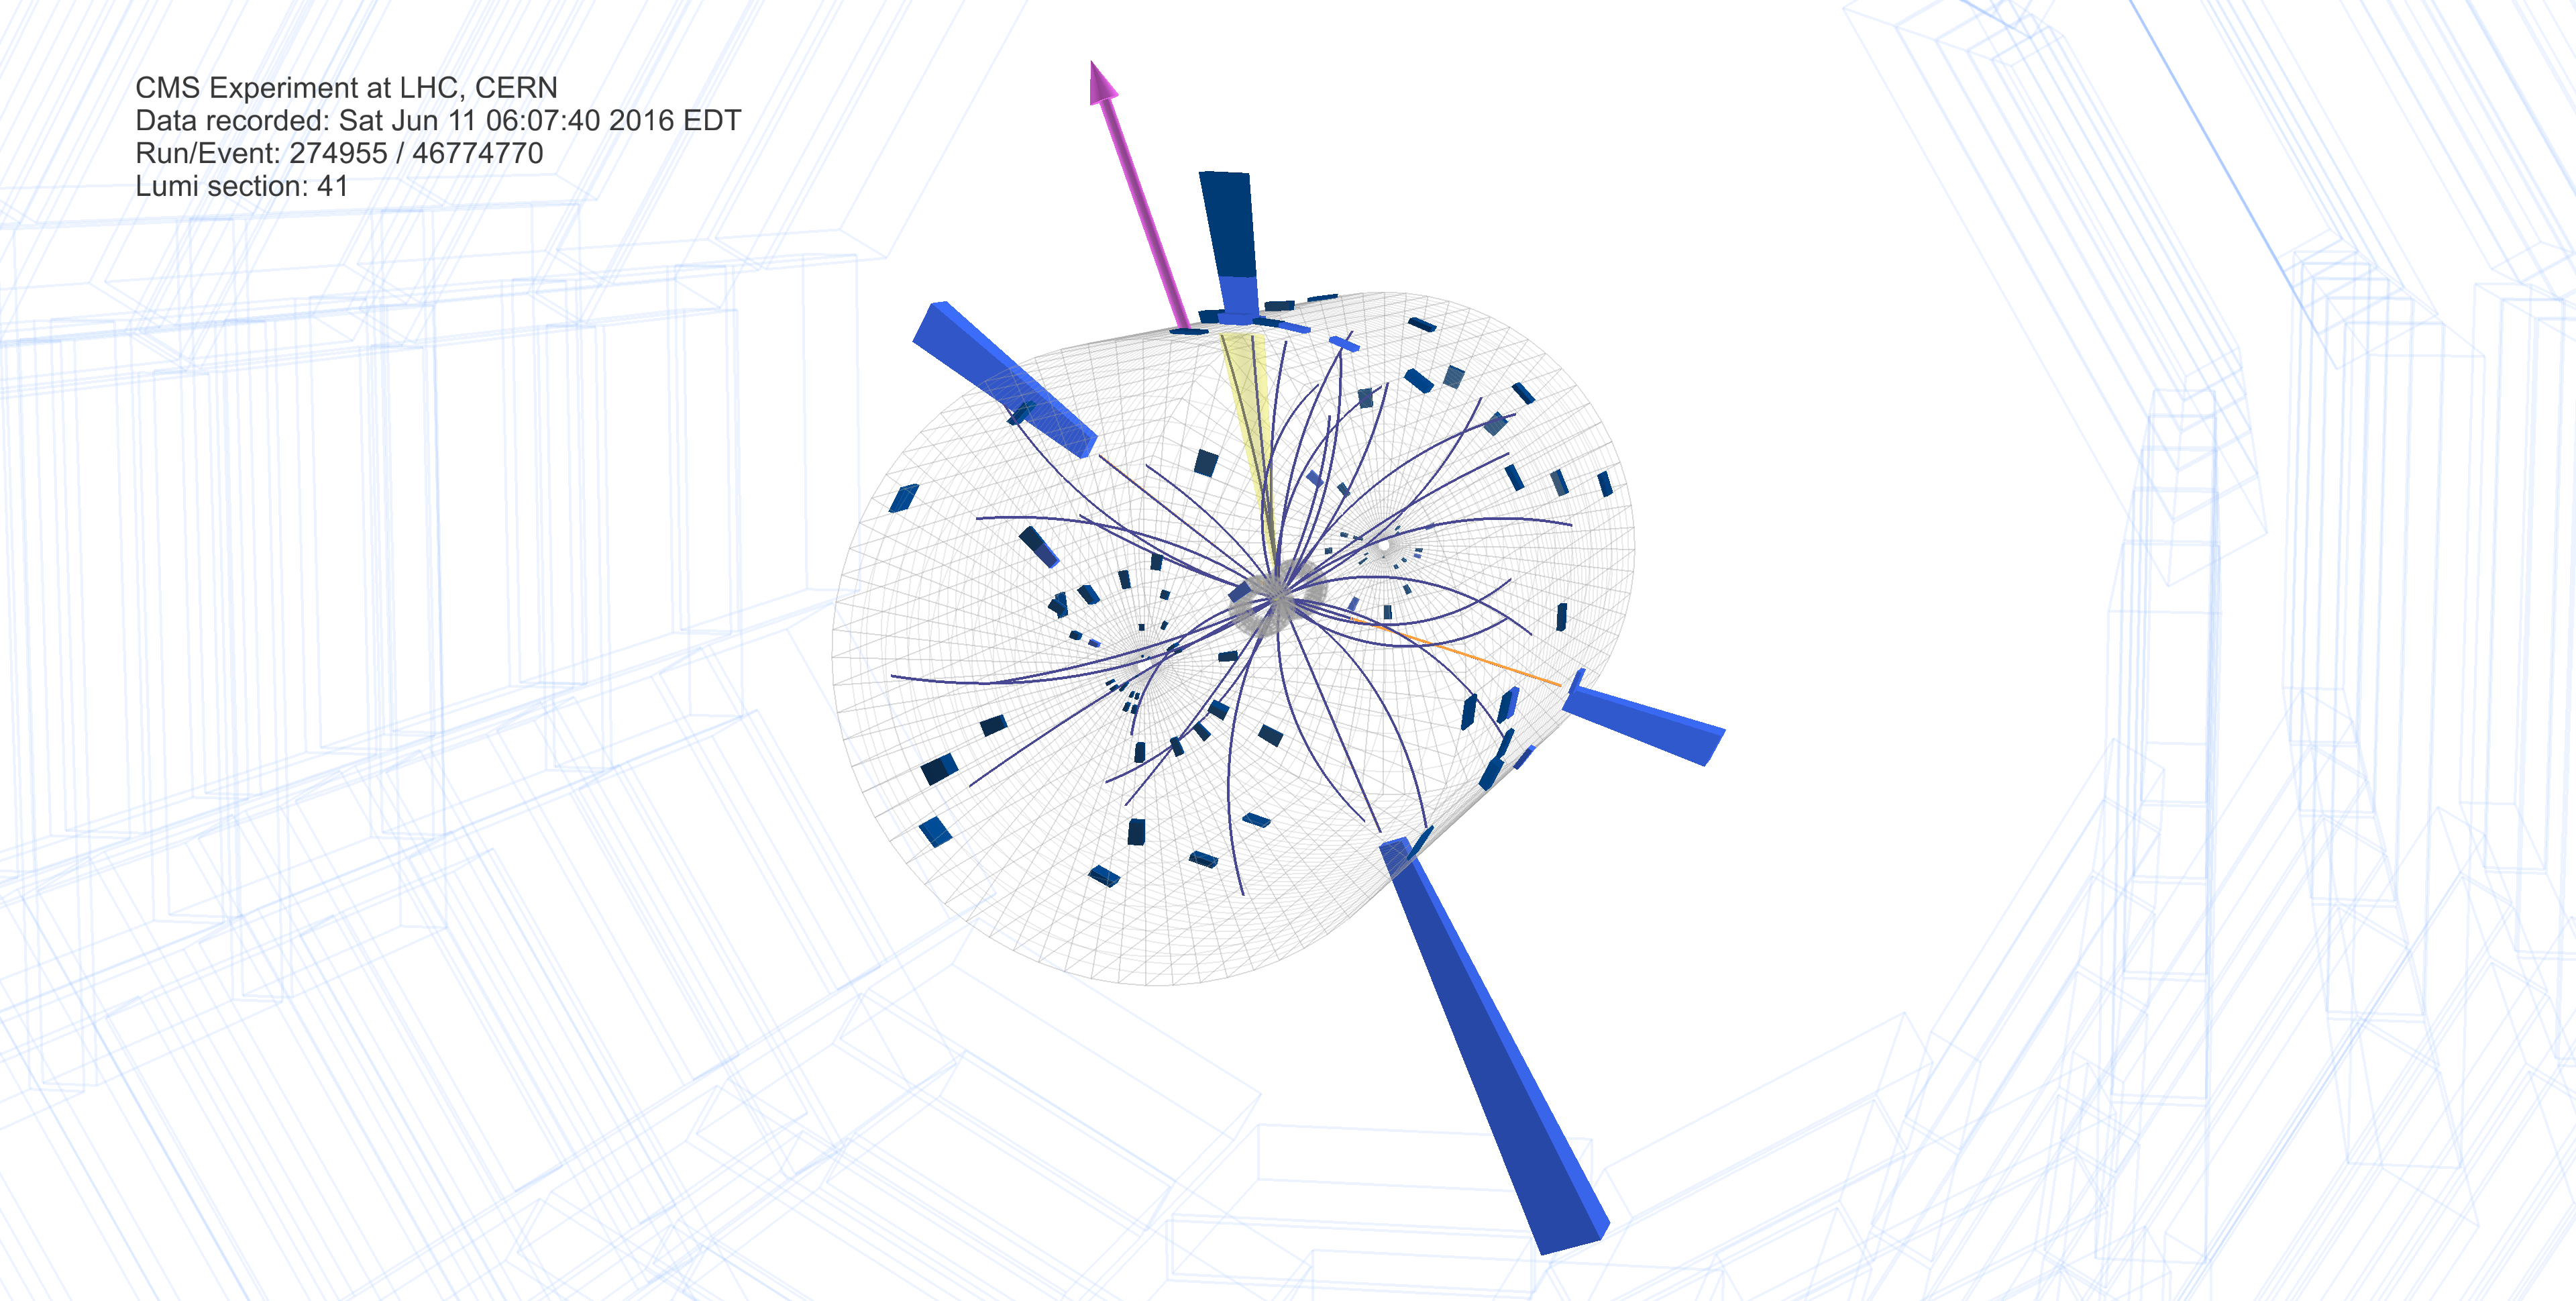
\includegraphics[width=1.0\textwidth]{figures/cmsShow_WevZee_ZpT200-274955_46774770_41_3DTower.png}}\vspace{1cm}

\fbox{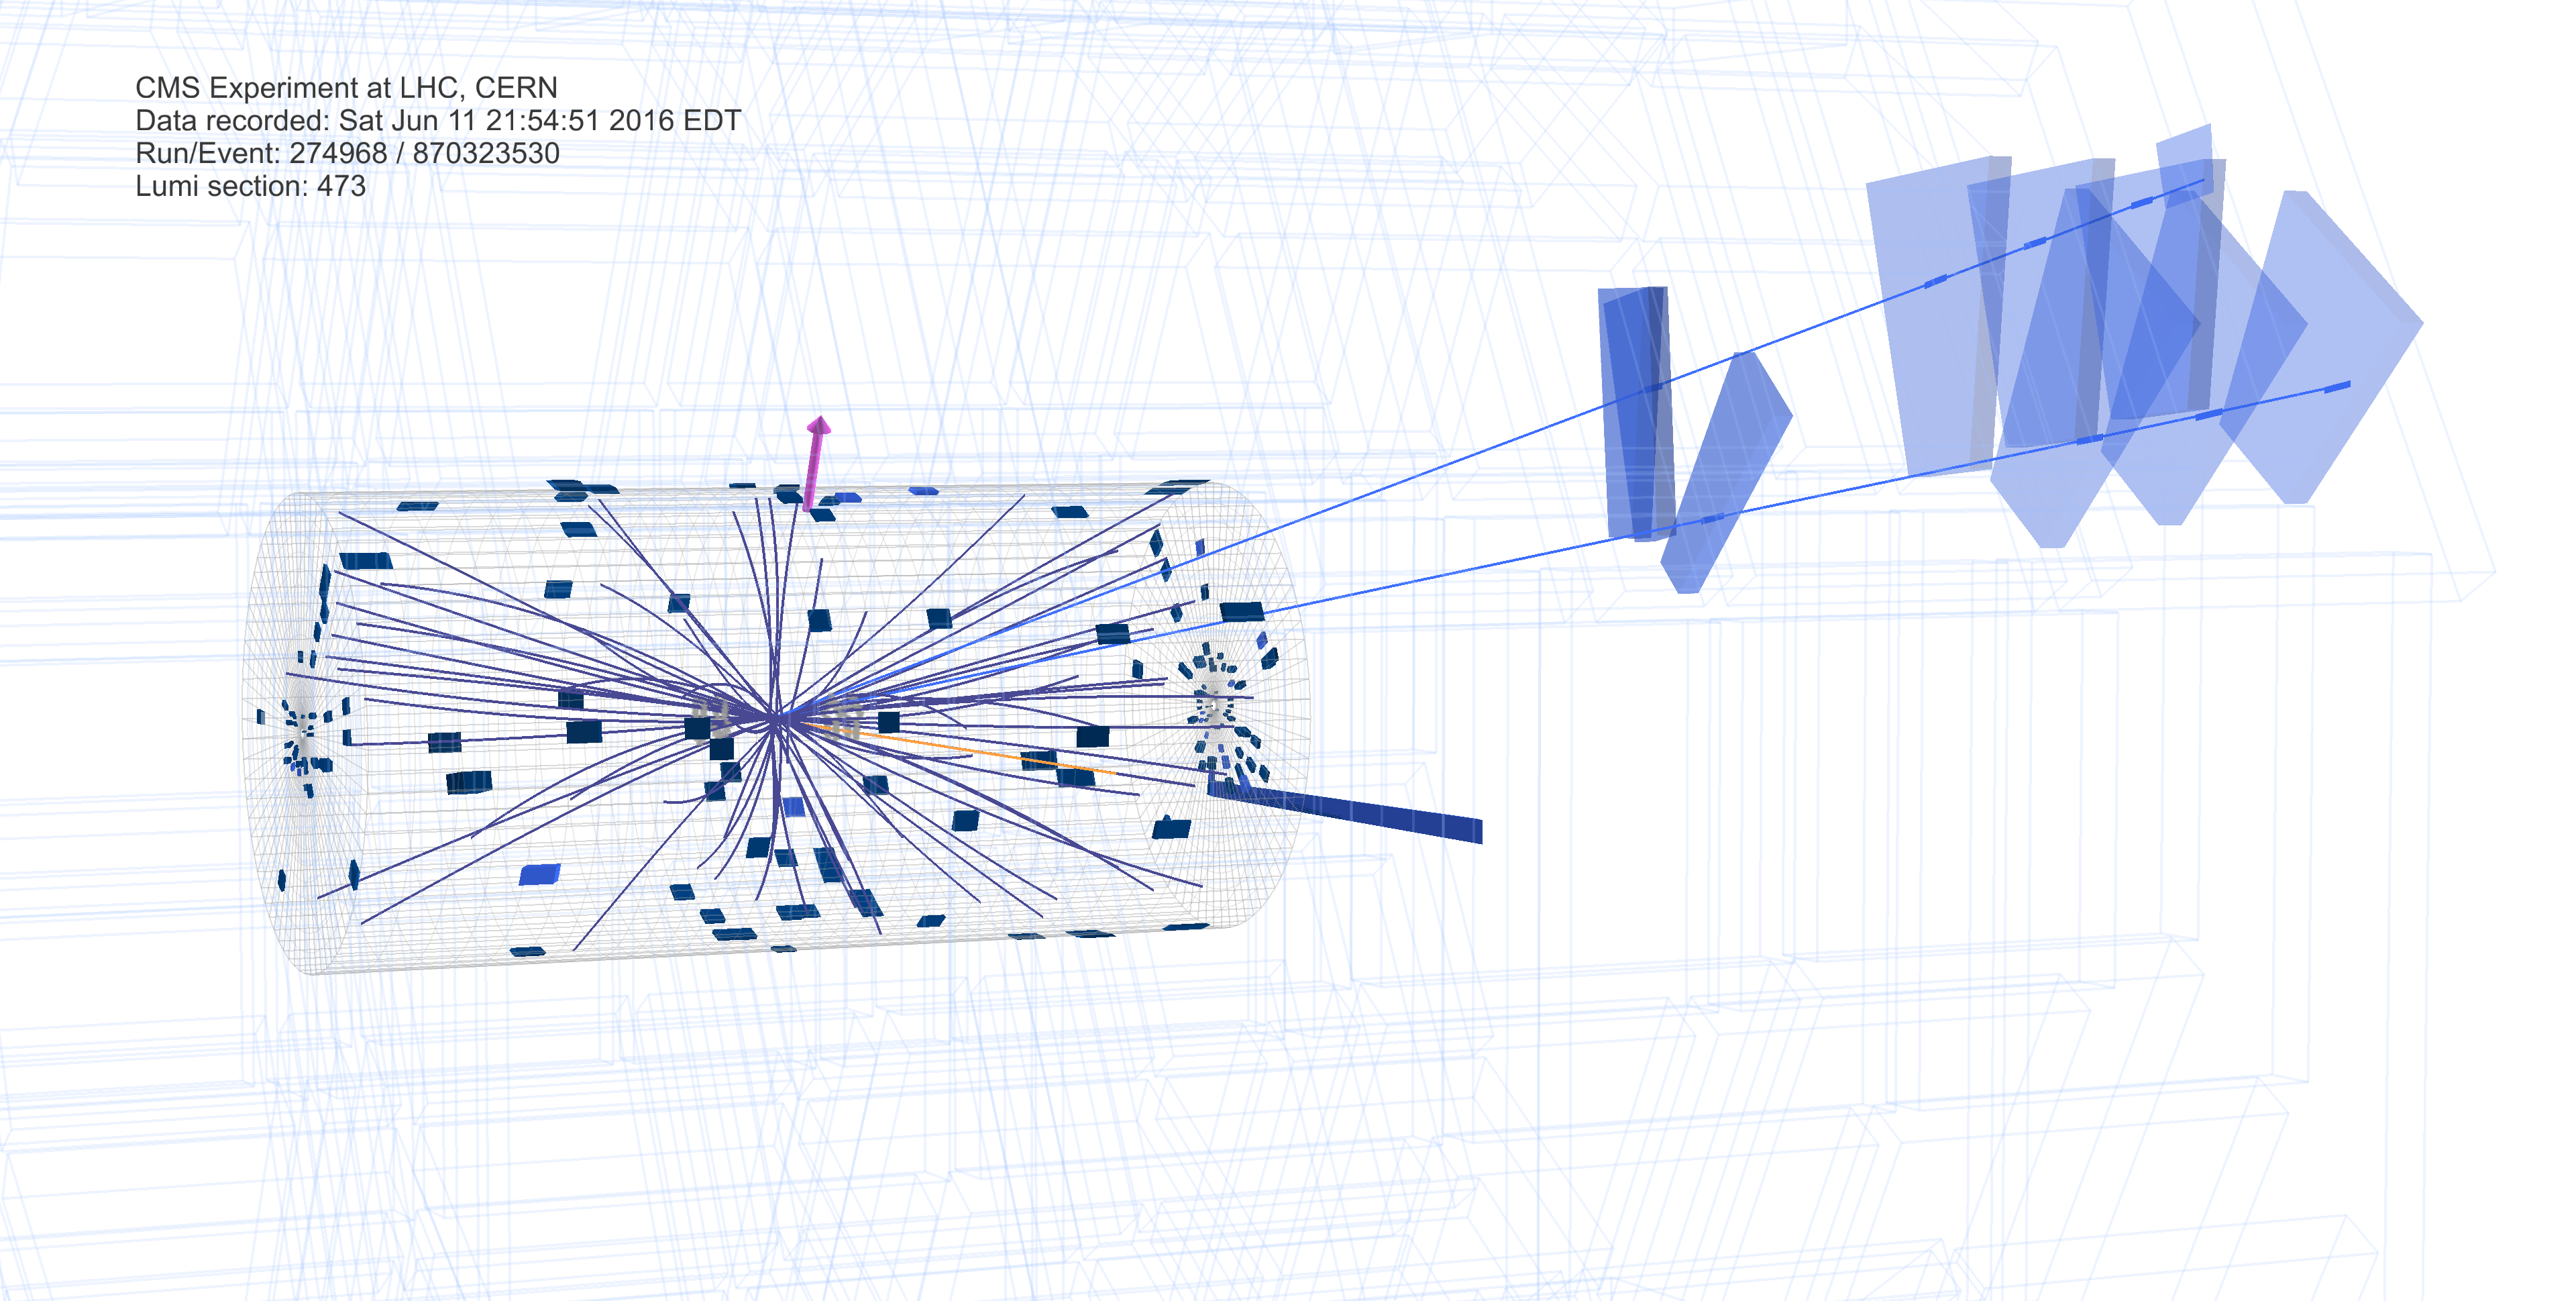
\includegraphics[width=1.0\textwidth]{figures/cmsShow_WevZmm_ZpT200-274968_870323530_473_3DTower.png}}\vspace{1cm}

\caption{3D event displays of W($\ell\nu$)Z($\ell\ell$) events with Z $p_\mathrm{T} > 200 \GeV$. 
\eventDisplayCaption
\label{fig:wz3l_eventdisplay}}
\end{figure}
\clearpage

